% =============================================================================
% CHAPTER 3 — METHODOLOGY
% a11y-autofix: A Multi-Agent Framework for Automated Web Accessibility
% Remediation in React/TypeScript Codebases
%
% Drop-in replacement for the current Chapter 3 placeholder.
% Include from the main thesis file with:  % =============================================================================
% CHAPTER 3 — METHODOLOGY
% a11y-autofix: A Multi-Agent Framework for Automated Web Accessibility
% Remediation in React/TypeScript Codebases
%
% Drop-in replacement for the current Chapter 3 placeholder.
% Include from the main thesis file with:  % =============================================================================
% CHAPTER 3 — METHODOLOGY
% a11y-autofix: A Multi-Agent Framework for Automated Web Accessibility
% Remediation in React/TypeScript Codebases
%
% Drop-in replacement for the current Chapter 3 placeholder.
% Include from the main thesis file with:  % =============================================================================
% CHAPTER 3 — METHODOLOGY
% a11y-autofix: A Multi-Agent Framework for Automated Web Accessibility
% Remediation in React/TypeScript Codebases
%
% Drop-in replacement for the current Chapter 3 placeholder.
% Include from the main thesis file with:  \input{chapter3_methodology}
% =============================================================================

\chapter{Methodology}
\label{chap:methodology}

This chapter presents the methodology underlying the design, implementation,
and evaluation of the automated accessibility repair framework developed in
this dissertation.  The methodology is structured across three complementary
dimensions: \emph{research design}, which establishes the epistemological
approach and experimental protocol; \emph{framework design}, which documents
the engineering decisions behind each system component; and \emph{evaluation
design}, which specifies how the framework's effectiveness is measured across
the four research questions.

The chapter proceeds as follows.  Section~\ref{sec:research_design} situates
the work within empirical software engineering and describes the overall
experimental protocol.  Section~\ref{sec:overview} provides an architectural
overview of the framework.  Sections~\ref{sec:prompt_template}
through~\ref{sec:validation_pipeline} describe each major component in detail:
the six-component prompt engineering template, the multi-tool detection
protocol, the adaptive repair routing engine, and the four-layer validation
pipeline.  Section~\ref{sec:experimental_design} specifies the experimental
variables, model selection criteria, and ablation study design.
Section~\ref{sec:dataset} documents the construction of the benchmark dataset.
Section~\ref{sec:metrics} defines all evaluation metrics.  Finally,
Section~\ref{sec:implementation} describes the implementation infrastructure
and deployment considerations.

% =============================================================================
\section{Research Design}
\label{sec:research_design}
% =============================================================================

\subsection{Research Paradigm and Strategy}

This dissertation adopts a \emph{design science} research paradigm
\cite{hevner2004design}, in which the primary output is an artefact—the
automated repair framework—and knowledge is generated through the rigorous
construction and evaluation of that artefact in realistic problem settings.
Design science is appropriate when the research goal is both to solve a
practical problem (the detection-correction gap identified in
Chapter~\ref{chap:intro}) and to produce generalisable knowledge about the
design choices that make the solution effective \cite{march1995design}.

The evaluation follows the \emph{empirical software engineering} tradition of
Wohlin et al.\ \cite{wohlin2012}, combining a controlled experiment on a
curated benchmark dataset with a quasi-experiment across multiple LLM
architectures under real-world conditions.  This mixed design enables both
internal validity—controlled conditions allow causal attribution of
performance differences to specific variables—and external validity—real-world
violations from open-source projects ensure ecological validity.

\subsection{Research Questions and Methodological Mapping}

The four research questions introduced in Section~\ref{sec:rq} govern the
experimental design.  Table~\ref{tab:rq_mapping} maps each research question
to the methodological component responsible for addressing it, the variables
it studies, and the metrics used to evaluate outcomes.

\begin{table}[htbp]
\caption{Mapping of research questions to methodological components,
  variables, and evaluation metrics.}
\label{tab:rq_mapping}
\centering\small
\renewcommand{\arraystretch}{1.3}
\begin{tabular}{p{0.05\textwidth}p{0.22\textwidth}p{0.18\textwidth}p{0.18\textwidth}p{0.20\textwidth}}
\toprule
\textbf{RQ} & \textbf{Question (summary)} & \textbf{Method. component} &
\textbf{Independent variable} & \textbf{Metric} \\
\midrule
RQ1 & Prompt transformation for repair
    & Prompt template design + ablation study
    & Template component presence/absence
    & Repair success rate, failure mode frequency \\
RQ2 & Prompting strategy comparison
    & Controlled experiment (zero-shot / few-shot / CoT)
    & Prompting strategy
    & Success rate, tokens used, generation time \\
RQ3 & LLM architecture comparison
    & Multi-model parallel experiment
    & LLM model identity
    & SR, MTTR, token cost, per-type SR \\
RQ4 & Issue category receptiveness
    & Stratified analysis by issue type
    & Issue type (7 categories)
    & IFR per category, failure mode distribution \\
\bottomrule
\end{tabular}
\end{table}

\subsection{Experimental Protocol}

The overall experimental protocol follows a five-phase pipeline:

\begin{enumerate}
  \item \textbf{Dataset construction}: Curate a benchmark corpus of real-world
    React/TypeScript files with confirmed accessibility violations
    (Section~\ref{sec:dataset}).
  \item \textbf{Detection}: Run the multi-tool scanner on all corpus files,
    producing deduplicated, confidence-annotated issue lists
    (Section~\ref{sec:detection_protocol}).
  \item \textbf{Prompt generation}: Apply the prompt engineering template to
    transform each issue list into a structured LLM prompt
    (Section~\ref{sec:prompt_template}).
  \item \textbf{Repair and validation}: Submit prompts to each experimental
    LLM, collect generated patches, and evaluate them through the four-layer
    validation pipeline (Section~\ref{sec:validation_pipeline}).
  \item \textbf{Analysis}: Aggregate metrics, compare conditions, and perform
    statistical tests (Section~\ref{sec:metrics}).
\end{enumerate}

\noindent
All phases are fully automated and reproducible.  The source code, benchmark
dataset, experiment configuration files, and analysis scripts are published
as a replication package (see Appendix).

% =============================================================================
\section{Framework Overview}
\label{sec:overview}
% =============================================================================

\subsection{Design Rationale}

The framework was designed around three guiding principles derived from the
failure mode analysis in Section~\ref{sec:intro} and from prior work on
LLM-based code repair \cite{xia2023,chen2023llm}:

\begin{description}
  \item[Non-invasiveness.] Repairs must be the minimal change that resolves
    the violation.  LLMs tend to over-engineer responses \cite{chen2023llm};
    the framework constrains generation through explicit prompt constraints and
    post-hoc validation.
  \item[Safety-first operation.] No change is written to disk unless it passes
    all four validation layers.  This prevents the introduction of regressions,
    which is identified as the most damaging failure mode for practitioners.
  \item[Context completeness.] The primary cause of poor LLM repairs is
    insufficient context \cite{xia2023}.  The framework systematically
    enriches minimal detection outputs—typically terse JSON violation codes—
    with file context, WCAG specifications, and concrete examples before
    querying any model.
\end{description}

\subsection{Layered Architecture}

The framework is organised into five functional layers, as depicted in
Figure~\ref{fig:architecture}.  Each layer has a well-defined input, output,
and responsibility contract, enabling independent testing and substitution of
components.

\begin{figure}[htbp]
\centering
\begin{tikzpicture}[node distance=0.65cm and 0.4cm,
    layer/.style={rectangle, draw=black!60, fill=#1,
                  text width=\linewidth*0.6, text centered,
                  rounded corners=3pt, minimum height=2.2em,
                  font=\small\bfseries},
    sublabel/.style={font=\scriptsize, text=black!70},
    arrow/.style={-{Stealth[length=2.5mm]}, thick, draw=black!60}]

  \def\layerwidth{10cm}

  \node[layer=gray!12] (cli)
    {Layer 5 — Interface\\
     \normalfont\scriptsize CLI (Typer), REST API, CI/CD hooks};

  \node[layer=blue!10, below=of cli] (orch)
    {Layer 4 — Orchestration\\
     \normalfont\scriptsize Pipeline · ExperimentRunner · asyncio event loop};

  \node[layer=cyan!12, below=of orch] (detect)
    {Layer 3 — Detection\\
     \normalfont\scriptsize MultiToolScanner · DetectionProtocol · deduplication};

  \node[layer=orange!12, below=of detect] (prompt)
    {Layer 2 — Prompt Engineering\\
     \normalfont\scriptsize PromptBuilder · 6-component template · few-shot selector};

  \node[layer=green!12, below=of prompt] (repair)
    {Layer 1 — Repair \& Validation\\
     \normalfont\scriptsize Router · Agents (DirectLLM / OpenHands / SWE-agent) · ValidationPipeline};

  \node[layer=purple!10, below=of repair] (infra)
    {Layer 0 — Infrastructure\\
     \normalfont\scriptsize LLM Registry · LocalLLMClient · Reporter};

  \foreach \from/\to in {cli/orch, orch/detect, detect/prompt, prompt/repair, repair/infra}
    \draw[arrow] (\from) -- (\to);

\end{tikzpicture}
\caption{Layered architecture of the a11y-autofix framework.
  Data flows downward from the interface layer to infrastructure;
  validation results propagate upward.}
\label{fig:architecture}
\end{figure}

\subsection{End-to-End Data Flow}

Figure~\ref{fig:dataflow} illustrates the complete data flow through the
system for a single React/TypeScript source file.  The pipeline begins with
file discovery and terminates with either a validated patch written to disk or
a structured failure report, depending on whether all validation layers pass.

\begin{figure}[htbp]
\centering
\begin{tikzpicture}[
    node distance=0.5cm and 1.0cm,
    proc/.style={rectangle, draw, fill=blue!8, rounded corners=3pt,
                 text width=5.5em, text centered, minimum height=2em,
                 font=\footnotesize},
    store/.style={rectangle, draw, fill=yellow!12,
                  text width=5.5em, text centered, minimum height=1.8em,
                  font=\footnotesize},
    dec/.style={diamond, draw, fill=orange!12, text width=3.5em,
                text centered, inner sep=1pt, font=\footnotesize},
    term/.style={rectangle, draw, fill=green!12, rounded corners=10pt,
                 text width=5.5em, text centered, minimum height=2em,
                 font=\footnotesize},
    fail/.style={rectangle, draw, fill=red!10, rounded corners=10pt,
                 text width=5.5em, text centered, minimum height=2em,
                 font=\footnotesize},
    arr/.style={-{Stealth[length=2mm]}, thick}]

  \node[proc] (discover) {File\\Discovery};
  \node[proc, right=1.2cm of discover] (scan) {Multi-Tool\\Scan};
  \node[proc, right=1.2cm of scan] (dedup) {Detection\\Protocol};
  \node[dec, right=1.2cm of dedup] (hasiss) {Issues?};

  \node[proc, below=1.0cm of hasiss] (prompt) {Prompt\\Construction};
  \node[proc, left=1.2cm of prompt] (route) {Router};
  \node[proc, left=1.2cm of route] (agent) {Agent\\Execution};
  \node[dec, left=1.2cm of agent] (valid) {Passes\\validation?};

  \node[term, below=1.0cm of valid] (write) {Write Patch\\to Disk};
  \node[fail, right=1.2cm of write] (retry) {Retry /\\Fallback};
  \node[store, right=1.2cm of retry] (report) {Generate\\Report};

  \draw[arr] (discover) -- (scan);
  \draw[arr] (scan) -- (dedup);
  \draw[arr] (dedup) -- (hasiss);
  \draw[arr] (hasiss) -- node[right,font=\scriptsize]{yes} (prompt);
  \draw[arr] (hasiss.north) -- ++(0,0.6) -| node[above,font=\scriptsize]{no} (report);
  \draw[arr] (prompt) -- (route);
  \draw[arr] (route) -- (agent);
  \draw[arr] (agent) -- (valid);
  \draw[arr] (valid) -- node[left,font=\scriptsize]{yes} (write);
  \draw[arr] (valid.east) -- node[above,font=\scriptsize]{no} (retry);
  \draw[arr] (retry) -- (report);
  \draw[arr] (write) -- ++(0,-0.6) -| (report);

\end{tikzpicture}
\caption{End-to-end data flow for a single source file.  The pipeline
  short-circuits when no issues are detected; failed validations trigger
  a configurable retry loop with agent fallback.}
\label{fig:dataflow}
\end{figure}

% =============================================================================
\section{Prompt Engineering Framework}
\label{sec:prompt_template}
% =============================================================================

\subsection{Motivation and Design Objectives}

The central claim of this dissertation—embodied in RQ1—is that raw detection
tool outputs are structurally insufficient for driving high-quality LLM
repairs, and that systematic prompt engineering can close this gap.  To
understand why, consider a typical output from a Pa11y accessibility scan:

\begin{verbatim}
{
  "code": "WCAG2AA.Principle2.Guideline2_4.2_4_4.H77",
  "message": "Check that the link text combined with the
              preceding heading identifies the purpose",
  "selector": "main > section:nth-child(3) > a:nth-child(2)"
}
\end{verbatim}

\noindent
This output identifies that a link element may violate WCAG success criterion
2.4.4 (\emph{Link Purpose (In Context)}).  However, an LLM receiving only
this JSON lacks critical information: the current text content of the link,
the heading that precedes it, whether the link is dynamically generated, the
target URL that should inform descriptive text, the React component structure
surrounding the element, and the codebase's conventions for accessible link
patterns.

Without these contextual dimensions, LLMs generate repairs that are
syntactically plausible but semantically incorrect—a phenomenon well-documented
in the code generation literature \cite{chen2023llm,xia2023}.  The six-
component template addresses each contextual dimension systematically.

\subsection{The Six-Component Prompt Template}

The prompt template is structured as a sequence of six components, each
targeting a specific class of LLM failure mode identified in the preliminary
analysis.  The design is grounded in prompt engineering research showing that
structured multi-component prompts substantially outperform unstructured
descriptions for code generation tasks \cite{brown2020,wei2022}.

\subsubsection{Component 1: Role Definition}

The first component establishes a precise expert persona for the model.
Role definition activates domain-relevant knowledge embedded in pre-training
\cite{wei2022} and has been shown empirically to reduce hallucination rates
in specialised domains \cite{white2023prompt}.  The role specification is
not generic (e.g., ``You are a helpful coding assistant'') but encodes three
critical attributes:

\begin{itemize}
  \item \textbf{Domain expertise}: The model is cast as an expert in both
    React/TypeScript development and WCAG 2.1 accessibility standards.
  \item \textbf{Operational context}: The role specifies that the model is
    performing automated code repair, not general advice, activating more
    conservative and precise generation behaviour.
  \item \textbf{Quality constraint}: The role explicitly prioritises
    correctness, minimal change, and functional preservation.
\end{itemize}

\noindent
Formally, the role definition $R$ is instantiated as:

\begin{quote}
  \textit{``You are an expert web accessibility engineer specialising in
  React and TypeScript.  Your task is to repair accessibility violations
  in production code while strictly preserving all existing functionality.
  You apply only the minimal change necessary to resolve each violation.
  You are deeply familiar with WCAG 2.1 Level AA success criteria and their
  implementation in React JSX.''}
\end{quote}

\subsubsection{Component 2: Violation Context}

The second component transforms the terse violation report into a rich,
structured description of the accessibility problem.  For each issue in the
file's issue list, the violation context component provides:

\begin{itemize}
  \item The full human-readable WCAG success criterion name and a plain-
    language explanation of the accessibility barrier it addresses.
  \item The issue type (from the seven-category taxonomy: \texttt{contrast},
    \texttt{aria}, \texttt{keyboard}, \texttt{label}, \texttt{semantic},
    \texttt{alt-text}, \texttt{focus}) and the associated repair complexity
    (\texttt{simple}, \texttt{moderate}, \texttt{complex}).
  \item The confidence level of the detection (\texttt{high}, \texttt{medium},
    \texttt{low}) with the number of independent tools that reported the issue.
  \item The CSS selector identifying the problematic element, enriched with
    the actual HTML context snippet extracted during scanning.
  \item The impact severity (critical, serious, moderate, minor) and the
    specific affected user population (e.g., screen reader users, keyboard-
    only users, users with low vision).
\end{itemize}

\noindent
The enrichment of detection outputs with impact descriptions and affected
populations is motivated by research showing that LLMs generate more
accessible and semantically correct code when the human consequence of
violations is made explicit \cite{feathers2024}.

\subsubsection{Component 3: Code Context}

The third component provides the source code that must be modified, together
with structural context that helps the model understand the codebase
architecture.  This component includes:

\begin{itemize}
  \item The complete content of the target file, framed within a markdown
    code block with language identifier (\texttt{```tsx}).
  \item The file path relative to the project root, which encodes information
    about the component's role in the application (e.g., a path containing
    \texttt{/layout/} implies the component contributes to page structure).
  \item A list of imported modules and components visible at the top of the
    file, enabling the model to reason about available APIs without access
    to the full codebase.
  \item If the component receives props, the TypeScript interface definition
    for those props, extracted via a lightweight AST analysis step.
\end{itemize}

\noindent
The decision to include the complete file rather than only the violating
element is justified by the finding of Xia et al.\ \cite{xia2023} that
models repair bugs correctly at significantly higher rates when the full
function is provided rather than only the buggy lines.  For accessibility
repairs specifically, the surrounding component logic determines whether a
proposed fix is semantically appropriate—a button's \texttt{aria-label}
must reflect its actual action, which requires understanding the surrounding
event handler.

\subsubsection{Component 4: Constraints}

The fourth component specifies explicit operational constraints that the model
must satisfy in its output.  The constraint set was derived empirically from
the preliminary failure mode analysis, with each constraint targeting a
specific failure pattern:

\begin{enumerate}
  \item \textbf{Minimal change constraint}: Modify only the elements
    identified in the violation report.  Do not restructure, rename, or
    refactor any code that is not directly related to the accessibility fix.
    \emph{Targets:} over-engineering failure mode.
  \item \textbf{Functional preservation constraint}: Preserve all existing
    event handlers, state management, prop interfaces, and rendering logic.
    The repaired file must be functionally equivalent to the original for
    all non-accessibility behaviour.
    \emph{Targets:} functional regression failure mode.
  \item \textbf{Framework convention constraint}: Use idiomatic React/JSX
    patterns.  Do not introduce raw DOM manipulation, vanilla JavaScript
    APIs incompatible with the React rendering model, or deprecated React
    patterns.
    \emph{Targets:} framework convention violation failure mode.
  \item \textbf{API existence constraint}: Use only ARIA attributes, HTML
    elements, and React APIs that are documented in the WCAG 2.1
    specification and in the React 18 documentation.
    \emph{Targets:} API hallucination failure mode.
  \item \textbf{Completeness constraint}: Return the complete modified file,
    not a partial snippet.  Do not use ellipsis (\texttt{...}) or placeholder
    comments to abbreviate unchanged sections.
    \emph{Targets:} incomplete output failure mode.
  \item \textbf{Format constraint}: Output exactly one code block delimited
    by \texttt{```tsx} and \texttt{```}.  Do not include explanation,
    comments, or prose outside this block.
    \emph{Targets:} parsing failure mode.
\end{enumerate}

\noindent
The explicit enumeration of constraints represents a departure from implicit
quality expectations common in informal prompting, and is motivated by
the finding that models adhere significantly better to explicit constraints
than to implied ones \cite{white2023prompt}.

\subsubsection{Component 5: Few-Shot Examples}

The fifth component provides between one and three concrete examples of
correctly repaired accessibility violations.  Few-shot prompting dramatically
reduces failure rates by demonstrating the expected repair pattern through
in-context learning \cite{brown2020,min2022rethinking}.

Example selection is not random.  Each example is drawn from a pre-constructed
library organised by issue type, and examples are selected for the current
prompt using \emph{semantic similarity}: the example whose violation
description most closely matches the current issue (measured by cosine
similarity in the embedding space of a lightweight sentence encoder) is
prioritised.  This approach, known as retrieval-augmented few-shot learning
\cite{min2022rethinking}, has been shown to outperform fixed example sets
by ensuring that demonstrations are relevant to the specific repair task.

Each example comprises:
\begin{itemize}
  \item The violation description (mirroring Component 2 format).
  \item The original non-compliant code snippet.
  \item The corrected code snippet.
  \item A brief annotation explaining \emph{what} was changed and \emph{why}
    it resolves the violation without affecting functionality.
\end{itemize}

\subsubsection{Component 6: Output Format Specification}

The sixth component closes the prompt with an explicit output format
specification.  While the constraints in Component 4 establish what the model
must produce, Component 6 specifies exactly how the output must be structured
to enable automated parsing and validation.  This component:

\begin{itemize}
  \item Restates the exact code block delimiters expected.
  \item Specifies that the output must be a valid, complete TypeScript/JSX
    file (not a fragment).
  \item Instructs the model to include a structured comment block immediately
    before the closing delimiter, enumerating the changes made and the WCAG
    criteria each change addresses.
  \item Specifies that if the model determines a violation is a false
    positive or cannot be repaired within the given constraints, it should
    output the original file unchanged and include a \texttt{// SKIP:}
    comment with a reason.
\end{itemize}

\noindent
The \texttt{SKIP} mechanism is an important design choice: it acknowledges that
LLMs should abstain rather than hallucinate a repair when a genuine solution
exceeds their capability.  Research on LLM calibration has shown that models
that express uncertainty produce better-calibrated outputs than models forced
to always generate an answer \cite{kadavath2022}.

\subsection{Template Composition and Assembly}

The six components are assembled dynamically per file.  Algorithm~\ref{alg:prompt}
describes the assembly process.  Note that few-shot examples (Component 5) are
adapted per issue type, and the constraint set (Component 4) is augmented with
violation-specific constraints derived from the issue's WCAG criterion.

\begin{algorithm}[htbp]
\caption{Prompt Assembly Algorithm}
\label{alg:prompt}
\begin{algorithmic}[1]
\Require $\mathcal{I}$: list of \texttt{A11yIssue} for file $f$, $\mathcal{E}$: few-shot example library
\Ensure structured prompt string $P$
\State $P \gets \text{RoleDefinition}()$
\For{each $i \in \mathcal{I}$}
  \State $P \gets P + \text{ViolationContext}(i)$
\EndFor
\State $P \gets P + \text{CodeContext}(f)$
\State $C_{\text{base}} \gets \text{BaseConstraints}()$
\For{each $i \in \mathcal{I}$}
  \State $C_{\text{base}} \gets C_{\text{base}} \cup \text{ViolationConstraints}(i.\text{wcag\_criteria})$
\EndFor
\State $P \gets P + C_{\text{base}}$
\State $\text{types} \gets \{i.\text{issue\_type} : i \in \mathcal{I}\}$
\State $\text{examples} \gets \emptyset$
\For{each $t \in \text{types}$}
  \State $e \gets \arg\max_{e' \in \mathcal{E}[t]} \text{sim}(e', \mathcal{I})$
  \State $\text{examples} \gets \text{examples} \cup \{e\}$
\EndFor
\State $P \gets P + \text{FewShotBlock}(\text{examples})$
\State $P \gets P + \text{OutputFormatSpec}()$
\State \Return $P$
\end{algorithmic}
\end{algorithm}

\subsection{Ablation Study Design}

To answer RQ1 quantitatively—specifically, to determine the contribution of
each template component—a component-level ablation study is conducted.  Seven
experimental conditions are evaluated: the complete six-component template
(baseline), and six reduced conditions in which each component is replaced
by a minimal placeholder or removed entirely.  Table~\ref{tab:ablation}
specifies the seven conditions.

\begin{table}[htbp]
\caption{Ablation study conditions for the prompt engineering template.
  A check mark ($\checkmark$) indicates the component is present in full;
  a dash (--) indicates it is absent or replaced by a placeholder.}
\label{tab:ablation}
\centering\small
\renewcommand{\arraystretch}{1.2}
\begin{tabular}{lcccccc}
\toprule
\textbf{Condition} & \textbf{C1: Role} & \textbf{C2: Viol.}
  & \textbf{C3: Code} & \textbf{C4: Const.} & \textbf{C5: Few-shot}
  & \textbf{C6: Format} \\
\midrule
Full (baseline) & $\checkmark$ & $\checkmark$ & $\checkmark$
  & $\checkmark$ & $\checkmark$ & $\checkmark$ \\
\textsf{no-role}      & --           & $\checkmark$ & $\checkmark$
  & $\checkmark$ & $\checkmark$ & $\checkmark$ \\
\textsf{no-context}   & $\checkmark$ & --           & $\checkmark$
  & $\checkmark$ & $\checkmark$ & $\checkmark$ \\
\textsf{no-code}      & $\checkmark$ & $\checkmark$ & --
  & $\checkmark$ & $\checkmark$ & $\checkmark$ \\
\textsf{no-constr}    & $\checkmark$ & $\checkmark$ & $\checkmark$
  & --           & $\checkmark$ & $\checkmark$ \\
\textsf{no-examples}  & $\checkmark$ & $\checkmark$ & $\checkmark$
  & $\checkmark$ & --           & $\checkmark$ \\
\textsf{no-format}    & $\checkmark$ & $\checkmark$ & $\checkmark$
  & $\checkmark$ & $\checkmark$ & -- \\
\bottomrule
\end{tabular}
\end{table}

\noindent
Each condition is evaluated on all benchmark violations using a single fixed
LLM (the best-performing model from the RQ3 evaluation), holding all other
variables constant.  The dependent variable is repair success rate as defined
in Section~\ref{sec:metrics}.

% =============================================================================
\section{Multi-Tool Detection Protocol}
\label{sec:detection_protocol}
% =============================================================================

\subsection{Rationale for Multi-Tool Integration}

Automated accessibility scanners are specialised static and dynamic analysis
tools, each designed with different internal heuristics, rule sets, and DOM
access strategies.  Prior research has consistently demonstrated that
individual tools have non-trivial false positive and false negative rates, and
that tool agreement varies substantially by violation category \cite{vigo2013}.
Sane et al.\ \cite{sane2023} found that different scanners detect largely
non-overlapping violation sets on the same pages, implying that any single
tool misses a substantial fraction of violations present.

These findings motivate the multi-tool consensus approach: by running multiple
independent scanners and aggregating their outputs, the framework achieves
both higher recall (more violations detected) and higher precision (violations
reported by multiple tools are almost certainly genuine).  The key insight
is that tool agreement functions as an empirical proxy for detection
confidence, analogous to the role of independent replication in experimental
science \cite{cohen1988}.

\subsection{Integrated Scanner Suite}

The framework integrates three accessibility scanning tools, selected to
provide complementary coverage of the WCAG criterion space:

\paragraph{Pa11y.}
Pa11y \cite{pa11y} is a command-line accessibility testing tool that uses
HTML\_CodeSniffer as its analysis engine, executing within a headless Chromium
browser environment.  Pa11y excels at detecting structural HTML conformance
issues—missing document structure, invalid ARIA roles, and absent form labels—
because HTML\_CodeSniffer operates on the raw DOM and can apply rule sets
corresponding to WCAG 2.0, WCAG 2.1, and Section 508 simultaneously.  Pa11y
outputs violations as JSON objects containing the WCAG guideline code (e.g.,
\texttt{WCAG2AA.Principle4.Guideline4\_1.4\_1\_2.H91.A.NoContent}), a
human-readable message, and the CSS selector of the violating element.  The
WCAG guideline code provides a direct mapping to the normative success
criterion, which is used as the primary key in the deduplication process.

\paragraph{Axe-core.}
Axe-core \cite{axe} is a JavaScript accessibility engine developed by Deque
Systems that evaluates the live DOM against a curated set of accessibility
rules.  Its design philosophy prioritises zero false positives over recall:
every rule in axe-core's rule set has been validated against hundreds of real-
world examples, and rules are only flagged when the engine is certain the
element fails accessibility requirements.  Axe-core enriches its output with
CSS selectors, contextual HTML snippets, impact severity ratings (critical,
serious, moderate, minor), and links to repair guidance documentation.  It
provides a rule identifier (e.g., \texttt{color-contrast}) that can be mapped
to the WCAG success criterion it implements.  In the framework, axe-core is
invoked both directly via a Node.js subprocess and through Playwright for
dynamic component evaluation.

\paragraph{Playwright + axe-core.}
React applications render components dynamically; the DOM state after
JavaScript execution may differ substantially from the static HTML snapshot.
Playwright \cite{playwright2023} provides a browser automation API that
enables evaluation of the fully rendered DOM, including components that
initialise state on mount, components that depend on user interaction to
reveal content, and components that use CSS-in-JS for styling.  The framework
configures Playwright to load each component file in an isolated sandbox,
execute all mount effects, and then inject axe-core to scan the rendered
output.  This two-step process captures violations that static scanners miss
due to React's virtual DOM model.

\subsection{Cross-Tool Deduplication}

The output of the three scanners for a single file is a multiset of raw
findings, potentially containing multiple reports of the same underlying
accessibility failure from different tools.  Without deduplication, the issue
list passed to the LLM would contain redundant and conflicting entries that
increase token consumption and confuse the model.

Deduplication is based on a \emph{content-addressed key} computed per finding:

\begin{equation}
  k(f) \;=\; \operatorname{normalise}\!\left(f.\texttt{selector}\right)
  \;\|\;
  \left(f.\texttt{wcag\_criteria} \parallel f.\texttt{rule\_id}\right)
  \label{eq:dedup_key}
\end{equation}

\noindent
where $\|$ denotes string concatenation with the separator \texttt{"|"},
$\parallel$ denotes priority-based selection (WCAG criterion is preferred;
rule identifier is used as a fallback when no WCAG mapping is available),
and $\operatorname{normalise}(\cdot)$ lowercases and strips whitespace from
the CSS selector.  Two findings with the same key $k$ are treated as
observations of the same accessibility failure, regardless of which tool
reported them.

The normalisation of CSS selectors is critical: Pa11y and axe-core may
generate different but semantically equivalent selector strings for the same
DOM element (e.g., \texttt{main > a:nth-child(3)} versus
\texttt{main~a.nav-link}).  The framework uses a selector canonicalisation
step—lowercasing, stripping pseudo-class arguments, and collapsing whitespace—
to maximise deduplication accuracy.

All findings sharing the same key $k$ are merged into a single
\texttt{A11yIssue} record.  A \emph{primary finding} is selected as the most
informative representative of the group using the prioritisation function:

\begin{equation}
  \text{primary}(G) = \arg\max_{f \in G}\;
    \Big( \mathbb{1}[f.\texttt{wcag\_criteria} \neq \emptyset],\;
          \text{impact\_rank}(f.\texttt{impact}),\;
          \left|f.\texttt{context}\right| \Big)
  \label{eq:primary}
\end{equation}

\noindent
The lexicographic maximisation first prefers findings with an explicit WCAG
criterion (which enables richer violation context generation), then higher
impact severity, then more informative context snippets.

\subsection{Issue Type Classification}

Each deduplicated issue is classified into one of seven issue types using a
hierarchical mapping:

\begin{enumerate}
  \item If the issue's WCAG criterion appears in the curated
    \texttt{WCAG\_TO\_ISSUE\_TYPE} mapping table (covering 40+ criteria),
    the mapped type is assigned.
  \item Otherwise, if the issue's rule identifier appears in the
    \texttt{RULE\_TO\_ISSUE\_TYPE} mapping table (covering 55+ axe-core and
    Pa11y rules), the mapped type is assigned.
  \item If neither mapping resolves, the issue is classified as
    \texttt{OTHER}.
\end{enumerate}

\noindent
Table~\ref{tab:issue_types} provides the full seven-category taxonomy with
representative WCAG success criteria, typical repair patterns, and the
complexity rating assigned to each type.  The complexity dimension informs the
routing decision described in Section~\ref{sec:router}.

\begin{table}[htbp]
\caption{Issue type taxonomy: seven categories with representative WCAG
  criteria, repair patterns, and complexity ratings.}
\label{tab:issue_types}
\centering\small
\renewcommand{\arraystretch}{1.3}
\begin{tabular}{lp{0.18\textwidth}p{0.22\textwidth}p{0.12\textwidth}}
\toprule
\textbf{Type} & \textbf{WCAG SC (examples)} & \textbf{Typical repair} & \textbf{Complexity} \\
\midrule
\texttt{alt-text}  & 1.1.1 Non-text content
  & Add/correct \texttt{alt} attribute & Simple \\
\texttt{label}     & 2.4.4 Link purpose; 2.5.3 Label in name
  & Add \texttt{aria-label} or \texttt{aria-labelledby} & Simple--Moderate \\
\texttt{aria}      & 4.1.2 Name, role, value; 4.1.3 Status messages
  & Correct ARIA role or attribute value & Simple \\
\texttt{keyboard}  & 2.1.1 Keyboard; 2.4.1 Bypass blocks
  & Add \texttt{tabIndex}, keyboard handler & Moderate \\
\texttt{focus}     & 2.4.7 Focus visible; 2.4.11 Focus appearance
  & Add/restore focus styles & Moderate \\
\texttt{semantic}  & 1.3.1 Info and relationships; 2.4.6 Headings
  & Restructure element hierarchy or roles & Moderate--Complex \\
\texttt{contrast}  & 1.4.3 Contrast minimum; 1.4.11 Non-text contrast
  & Modify colour values, CSS variables & Complex \\
\bottomrule
\end{tabular}
\end{table}

\subsection{Confidence Assignment via Tool Consensus}

A critical design requirement of the detection protocol is the assignment of
calibrated confidence levels to each deduplicated issue.  Confidence serves
two purposes: it informs the routing decision (high-confidence issues of
complex types are routed to more capable agents) and it signals to the LLM
which violations most warrant correction when context window constraints
require prioritisation.

Confidence is computed according to Equation~\ref{eq:confidence}:

\begin{equation}
  \mathrm{confidence}(T,\,\texttt{impact}) =
  \begin{cases}
    \textsc{High}   & \text{if } |T| \geq \tau_{\min} \\[4pt]
    \textsc{Medium} & \text{if } |T| = 1 \;\wedge\; \texttt{impact}
                      \in \{\text{critical},\, \text{serious}\} \\[4pt]
    \textsc{Low}    & \text{otherwise}
  \end{cases}
  \label{eq:confidence}
\end{equation}

\noindent
where $T$ is the set of distinct scanners that reported the issue and
$\tau_{\min}$ is the minimum consensus threshold (default: $\tau_{\min} = 2$,
configurable).  The \textsc{Medium} tier captures high-severity violations
detected by a single tool: while cross-tool validation is absent, the high
impact severity provides independent evidence that the finding is likely
genuine, since axe-core's zero-false-positive design \cite{axe} means that
even single-tool detections of critical violations are highly reliable.

\subsection{Stable Issue Identifiers}

Each issue is assigned a stable, content-addressed identifier to support
longitudinal tracking across scan iterations:

\begin{equation}
  \mathrm{id}(i) = \mathrm{SHA\text{-}256}\!\left(
    f.\texttt{path} \;\|\; i.\texttt{selector} \;\|\;
    i.\texttt{wcag\_criteria} \;\|\; i.\texttt{issue\_type}
  \right)[{:}16]
  \label{eq:issue_id}
\end{equation}

The 16-character hexadecimal truncation ($2^{64}$ collision resistance)
provides stability across scans—the same issue in the same file always
receives the same identifier, enabling automatic detection of regressions
(previously fixed issues reappearing) without database infrastructure.

\subsection{Deterministic Issue Ordering}

To ensure that experiment outputs are reproducible across runs, issues are
sorted by the composite key:

\begin{equation}
  \text{sort key}(i) = \bigl(
    -\text{conf\_rank}(i.\texttt{confidence}),\;\;
    -\text{imp\_rank}(i.\texttt{impact}),\;\;
    i.\texttt{wcag\_criteria},\;\;
    i.\texttt{selector}
  \bigr)
  \label{eq:sort_key}
\end{equation}

\noindent
The sort places high-confidence, high-impact issues first, ensuring that when
token limits require truncation, the most important issues remain in the prompt.

% =============================================================================
\section{Adaptive Repair Routing}
\label{sec:router}
% =============================================================================

\subsection{Motivation: Agent Capability Heterogeneity}

Not all accessibility violations benefit from the same repair strategy.
A missing \texttt{alt} attribute on an image element is a localised,
single-attribute insertion that requires no understanding of surrounding
component logic.  A colour contrast failure, by contrast, may require
tracing colour values through CSS variables, design token files, and theme
configuration objects that span multiple files.  Using a wide-context,
multi-file agent for simple attribute insertions wastes computational
resources; using a surgical single-file editor for contrast fixes
produces incorrect repairs that address the symptom rather than the root cause.

The \emph{Router} component addresses this heterogeneity by automatically
selecting among three repair agents based on a quantitative analysis of each
file's issue set characteristics.

\subsection{Agent Profiles}

\paragraph{DirectLLMAgent.}
The DirectLLMAgent is the simplest repair strategy: it assembles the full
six-component prompt and queries the configured LLM through the
\texttt{LocalLLMClient} abstraction, requesting a complete corrected file.
No external tool invocation or multi-step planning is performed.  The agent
applies a lightweight TypeScript/JSX well-formedness check to the raw output,
extracts the code block, and writes the result.  DirectLLMAgent is used for
\texttt{simple}-complexity issues and as the universal fallback agent when
both specialist agents fail.

\paragraph{OpenHandsAgent.}
OpenHands \cite{openhands2024} is a coding agent that operates in a sandboxed
environment equipped with a shell, file system, and browser.  The agent
communicates with a running OpenHands server via its HTTP REST API.
OpenHandsAgent is selected for wide-context, multi-file repair tasks—
particularly \texttt{contrast} and \texttt{semantic} issues—because OpenHands
can autonomously navigate the project structure, read theme configuration files,
trace CSS variable definitions, and apply coordinated changes across multiple
files.  The OpenHands sandbox enables multi-step planning: it can inspect
related files, formulate a repair strategy, apply changes, and validate the
result before reporting success.

\paragraph{SWEAgent.}
SWE-agent \cite{sweagent} provides an Agent-Computer Interface (ACI) that
connects an LLM to a shell and a file editor optimised for surgical,
line-targeted edits.  The ACI provides commands for viewing file regions,
finding patterns, and applying minimal edits, preventing the agent from
receiving irrelevant context that would dilute its attention.  SWEAgent is
invoked via CLI subprocess; the framework captures the resulting \texttt{git
diff} and applies it programmatically.  SWEAgent is selected for localised
attribute and label issues where precision is more important than context width.

\subsection{The Scoring Matrix}

The Router computes an integer score for each file's \texttt{ScanResult} by
evaluating a set of additive and subtractive scoring factors.  The score is
interpreted as follows:

\begin{equation}
  \text{agent}(\text{score}) =
  \begin{cases}
    \texttt{openhands} & \text{if score} \geq 3 \\
    \texttt{swe-agent} & \text{if score} < 3
  \end{cases}
  \label{eq:routing}
\end{equation}

Table~\ref{tab:scoring} defines each scoring factor with its value and
justification.  The threshold of 3 was determined empirically to partition the
expected issue distribution roughly equally between agents across a calibration
set of 50 representative files.

\begin{table}[htbp]
\caption{Router scoring matrix: factors, values, and justifications.}
\label{tab:scoring}
\centering\small
\renewcommand{\arraystretch}{1.3}
\begin{tabular}{p{0.35\textwidth}rp{0.42\textwidth}}
\toprule
\textbf{Factor} & \textbf{Score} & \textbf{Justification} \\
\midrule
Issue set contains \texttt{contrast} or \texttt{semantic} types
  & $+4$ & These types require multi-file context; always route to OpenHands \\
Issue count $\geq \tau$ (\texttt{swe\_max\_issues}, default 4)
  & $+4$ & High-volume repairs exceed SWE-agent's per-session edit budget \\
Issue count $\geq 2\tau$
  & $+5$ & Very high volume; additional bonus to ensure OpenHands routing \\
At least one issue with \texttt{complex} complexity
  & $+3$ & Complex repairs require planning beyond file-level context \\
$\geq$3 distinct issue types present
  & $+3$ & Diverse issue sets require cross-concern reasoning \\
All issues of types \texttt{aria}, \texttt{label}, or \texttt{alt-text} AND count $< \tau$
  & $-3$ & Fully localized attribute fixes; SWE-agent is more efficient \\
\bottomrule
\end{tabular}
\end{table}

Figure~\ref{fig:routing_examples} visualises the routing decision for six
representative issue set configurations, illustrating how the scoring matrix
handles common cases across the complexity spectrum.

\begin{figure}[htbp]
\centering
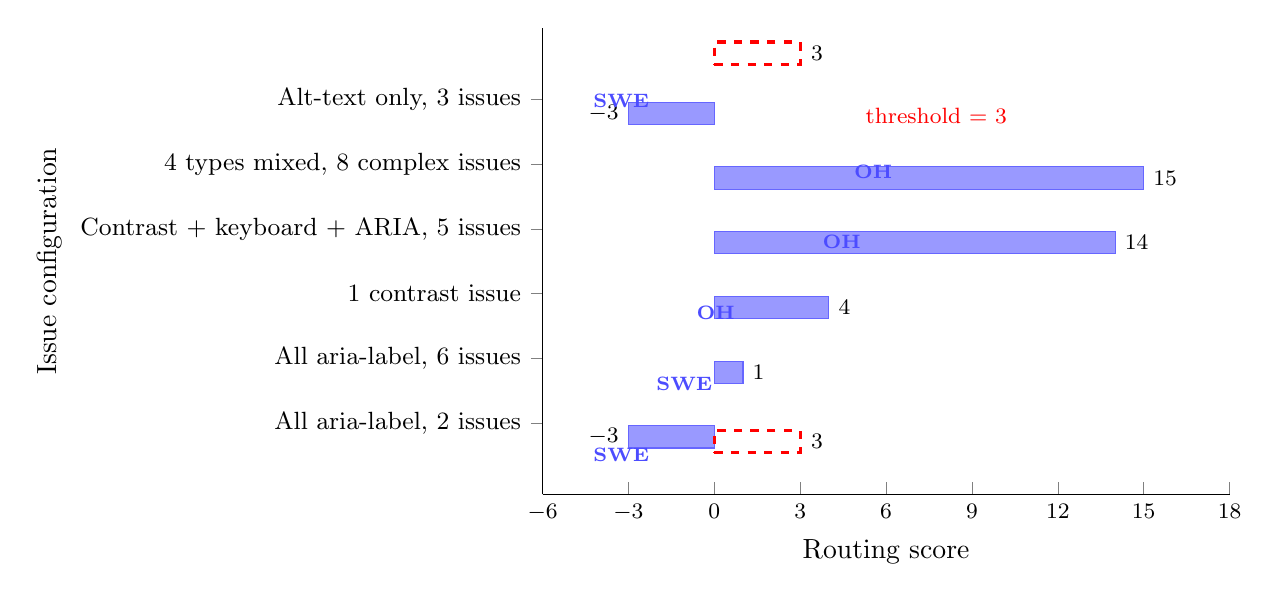
\begin{tikzpicture}
\begin{axis}[
  xbar,
  width=0.85\linewidth,
  height=7.5cm,
  xmin=-6, xmax=18,
  xlabel={Routing score},
  ylabel={Issue configuration},
  ytick=data,
  yticklabels={
    {All aria-label, 2 issues},
    {All aria-label, 6 issues},
    {1 contrast issue},
    {Contrast + keyboard + ARIA, 5 issues},
    {4 types mixed, 8 complex issues},
    {Alt-text only, 3 issues}
  },
  yticklabel style={font=\small},
  nodes near coords,
  nodes near coords align={horizontal},
  nodes near coords style={font=\footnotesize},
  bar width=8pt,
  axis y line*=left,
  axis x line*=bottom,
  xtick={-6,-3,0,3,6,9,12,15,18},
  xticklabel style={font=\footnotesize},
  legend style={at={(0.98,0.02)}, anchor=south east, font=\small},
]
\addplot[fill=blue!40, draw=blue!60] coordinates {
  (-3, 0) (1, 1) (4, 2) (14, 3) (15, 4) (-3, 5)
};
\addplot[fill=none, draw=red, dashed, very thick] coordinates {
  (3, -0.5) (3, 5.5)
};
\end{axis}
\node[font=\footnotesize, text=red] at (5.0, 4.8) {threshold = 3};
\node[font=\scriptsize, text=blue!70] at (1.0, 0.5) {\textbf{SWE}};
\node[font=\scriptsize, text=blue!70] at (1.8, 1.4) {\textbf{SWE}};
\node[font=\scriptsize, text=blue!70] at (2.2, 2.3) {\textbf{OH}};
\node[font=\scriptsize, text=blue!70] at (3.8, 3.2) {\textbf{OH}};
\node[font=\scriptsize, text=blue!70] at (4.2, 4.1) {\textbf{OH}};
\node[font=\scriptsize, text=blue!70] at (1.0, 5.0) {\textbf{SWE}};
\end{tikzpicture}
\caption{Router scoring for six representative issue configurations.
  Scores below the dashed threshold (3) route to SWE-agent;
  scores at or above route to OpenHands (OH).}
\label{fig:routing_examples}
\end{figure}

\subsection{Retry Protocol and Agent Fallback}

All agent invocations are wrapped in a configurable retry loop with maximum
$R$ attempts (default $R = 3$).  After each failed attempt, only the
unresolved subset of issues is re-submitted, preserving any progress made on
other issues in the same file.  If all $R$ attempts fail:

\begin{enumerate}
  \item If the selected agent was OpenHands, the system attempts one fallback
    invocation with SWEAgent.
  \item If the selected agent was SWEAgent, or if the SWEAgent fallback also
    fails, the system makes one final attempt with DirectLLMAgent.
  \item If DirectLLMAgent also fails, the file is marked as \texttt{repair\_failed}
    and a full diagnostic report is generated.
\end{enumerate}

This cascade ensures graceful degradation: the most capable available agent
always receives a repair attempt, but partial failures do not silently
propagate to the output.

% =============================================================================
\section{Four-Layer Validation Pipeline}
\label{sec:validation_pipeline}
% =============================================================================

\subsection{Rationale for Multi-Layer Validation}

LLMs generate plausible but incorrect outputs with non-negligible probability.
For automated code repair, this translates directly into regressions:
functionality that worked before the repair stops working after it.  In a
production accessibility remediation context, regressions are typically
considered more harmful than unrepaired violations, since they introduce new
defects rather than merely leaving existing ones unresolved.

The four-layer validation pipeline implements a series of increasingly strict
checks that collectively filter the most common LLM failure modes identified
in the preliminary analysis.  A patch passes validation only if it clears all
four layers; partial success is not accepted.  The layers are ordered from
least to most computationally expensive, minimising total validation cost by
rejecting obvious failures early.

\subsection{Layer 1: Syntactic Validation}

The first layer verifies that the generated output is a well-formed TypeScript
JSX file.  It consists of three checks:

\begin{itemize}
  \item \textbf{Code block extraction}: The output is parsed to extract the
    content between \texttt{```tsx} and \texttt{```} delimiters.  If no such
    block is found, or if multiple conflicting blocks are found, the output is
    rejected.  This check targets the \emph{incomplete output} and
    \emph{format violation} failure modes.
  \item \textbf{Non-empty content}: The extracted content must be non-empty
    and must contain at least one import statement or JSX expression.
  \item \textbf{Heuristic JSX well-formedness}: A lightweight check verifies
    balanced brace nesting, the absence of unclosed JSX tags (detected via
    simple parenthesis/bracket balance tracking), and the absence of
    double-quoted \texttt{```} sequences inside the code block (a common
    artefact of models that misformat their output).  This is a heuristic
    rather than a full parse to minimise latency; full TypeScript compilation
    is deferred to Layer 2.
\end{itemize}

\subsection{Layer 2: Functional Preservation}

The second layer verifies that the repair preserves the functional behaviour
of the original component.  This is the most critical validation layer, as
functional regressions are the most damaging failure mode.  The layer
implements three checks:

\begin{itemize}
  \item \textbf{Prop interface preservation}: The TypeScript interface
    definition of the component's props (extracted from the original file via
    AST analysis) must be identical in the repaired file.  Any addition,
    removal, or type change of a prop is a regression indicator.
  \item \textbf{Export signature preservation}: The component's default export
    and any named exports must remain present with identical signatures.
    Missing exports would cause import failures in the consuming codebase.
  \item \textbf{Event handler preservation}: All \texttt{onClick}, \texttt{onChange},
    \texttt{onSubmit}, and other event handler identifiers present in the
    original file must be present in the repaired file.  This check prevents
    the common failure mode where a model rewrites the component from scratch,
    omitting event handlers that it deems unnecessary.
\end{itemize}

\subsection{Layer 3: Domain Verification}

The third layer verifies that the repair actually addresses the accessibility
violations rather than producing an output that passes syntactic checks but
ignores the violations.  This layer uses heuristic pattern matching rather
than full re-scanning (which would be too slow for the validation loop):

\begin{itemize}
  \item For \texttt{alt-text} violations: the repaired file must contain an
    \texttt{alt} attribute on the element identified by the violation's CSS
    selector.
  \item For \texttt{aria} violations: the repaired file must contain the
    specific ARIA attribute flagged by the violation (e.g.,
    \texttt{aria-label}, \texttt{role}).
  \item For \texttt{label} violations: the repaired file must contain an
    accessible name association (either \texttt{aria-label},
    \texttt{aria-labelledby}, or a \texttt{<label>} element with a
    \texttt{htmlFor} attribute).
  \item For \texttt{contrast} violations: the repair must modify at least one
    colour-related property on the element (CSS colour value, class name
    referencing a colour token, or a theme variable assignment).
\end{itemize}

The domain verification layer does not attempt to re-run the full scanner
suite, as this would multiply validation time by 3--5x.  Instead, it provides
a lightweight proxy check.  Full scanner re-evaluation is conducted separately
as part of the closed-loop evaluation described in Section~\ref{sec:metrics}.

\subsection{Layer 4: Code Quality Assessment}

The fourth layer assesses code quality attributes that are not captured by
the previous layers but are critical for production code acceptance:

\begin{itemize}
  \item \textbf{TypeScript compilation}: The repaired file is passed to the
    TypeScript compiler in \texttt{--noEmit} mode to detect type errors
    introduced by the repair.  Type errors often indicate that the model
    introduced incorrect prop usage or invalid API calls.
  \item \textbf{Complexity delta}: The cyclomatic complexity of the repaired
    file is computed and compared to the original.  If the repaired file's
    complexity exceeds the original by more than a configurable threshold
    (default: $+3$), the repair is flagged for review.  Significant complexity
    increases are a signal of over-engineering.
  \item \textbf{Added code ratio}: The ratio of added lines to removed lines
    in the diff must not exceed a configurable ceiling (default: $10\times$).
    Repairs that add ten times more code than they remove are unlikely to
    be minimal, violating the non-invasiveness principle.
\end{itemize}

Figure~\ref{fig:validation_flow} summarises the four-layer pipeline with
rejection paths.

\begin{figure}[htbp]
\centering
\begin{tikzpicture}[
    node distance=0.55cm,
    layer/.style={rectangle, draw, fill=blue!8, rounded corners=3pt,
                  text width=8em, text centered, minimum height=2.2em,
                  font=\small},
    check/.style={diamond, draw, fill=orange!12, text width=3.8em,
                  text centered, inner sep=1pt, font=\scriptsize},
    pass/.style={rectangle, draw, fill=green!12, rounded corners=8pt,
                 text width=6em, text centered, minimum height=1.8em,
                 font=\small},
    fail/.style={rectangle, draw, fill=red!10, rounded corners=8pt,
                 text width=6em, text centered, minimum height=1.8em,
                 font=\small},
    arr/.style={-{Stealth[length=2mm]}, thick},
    failarr/.style={-{Stealth[length=2mm]}, thick, draw=red!60, dashed}]

  \node[layer] (l1) {Layer 1\\Syntactic};
  \node[check, right=1.2cm of l1] (c1) {pass?};
  \node[layer, right=1.2cm of c1] (l2) {Layer 2\\Functional};
  \node[check, right=1.2cm of l2] (c2) {pass?};

  \node[layer, below=1.5cm of l1] (l3) {Layer 3\\Domain};
  \node[check, right=1.2cm of l3] (c3) {pass?};
  \node[layer, right=1.2cm of c3] (l4) {Layer 4\\Quality};
  \node[check, right=1.2cm of l4] (c4) {pass?};

  \node[pass, below=1.5cm of l4] (ok) {Patch\\Accepted};
  \node[fail, left=1.2cm of ok] (reject) {Reject /\\Retry};

  \draw[arr] (l1) -- (c1);
  \draw[arr] (c1) -- node[above,font=\scriptsize]{yes} (l2);
  \draw[arr] (l2) -- (c2);
  \draw[arr] (c2) -- node[right,font=\scriptsize]{yes} ++(0,-0.5)
    -| (l3);
  \draw[arr] (l3) -- (c3);
  \draw[arr] (c3) -- node[above,font=\scriptsize]{yes} (l4);
  \draw[arr] (l4) -- (c4);
  \draw[arr] (c4) -- node[right,font=\scriptsize]{yes} (ok);

  \draw[failarr] (c1.south) -- node[right,font=\scriptsize,text=red]{no}
    ++(0,-0.4) -| (reject.north);
  \draw[failarr] (c2.south) -- node[right,font=\scriptsize,text=red]{no}
    ++(0,-0.4) -- (reject.east |- c2) -- (reject.east);
  \draw[failarr] (c3.south) -- node[right,font=\scriptsize,text=red]{no}
    ++(0,-0.3) -- (reject);
  \draw[failarr] (c4.south) -- node[right,font=\scriptsize,text=red]{no}
    ++(0,-0.4) -- (reject.east |- c4) -- (reject.east);

\end{tikzpicture}
\caption{The four-layer validation pipeline.  Each layer applies
  progressively more thorough checks; a rejection at any layer triggers
  the retry/fallback mechanism.}
\label{fig:validation_flow}
\end{figure}

% =============================================================================
\section{Experimental Design}
\label{sec:experimental_design}
% =============================================================================

\subsection{Experimental Variables}

The experiment controls four independent variables corresponding to the four
research questions:

\begin{description}
  \item[IV1 — Template component presence] (RQ1): Binary per-component,
    yielding the seven ablation conditions in Table~\ref{tab:ablation}.
  \item[IV2 — Prompting strategy] (RQ2): Categorical with three levels:
    \emph{zero-shot} (Components 1--4 + 6, no examples), \emph{few-shot}
    (full six-component template), and \emph{chain-of-thought} (few-shot
    with an additional reasoning-elicitation instruction appended).
  \item[IV3 — LLM model identity] (RQ3): The set of models included in the
    multi-model experiment (see Section~\ref{sec:model_selection}).
  \item[IV4 — Issue type] (RQ4): Categorical with seven levels per the
    taxonomy in Table~\ref{tab:issue_types}.
\end{description}

\noindent
Dependent variables are defined in Section~\ref{sec:metrics}.

\subsection{Model Selection}
\label{sec:model_selection}

Model selection follows three criteria:
\begin{enumerate}
  \item \textbf{Local deployability}: All models must be deployable on
    commodity hardware (single consumer GPU with 16--24 GB VRAM) to support
    privacy-preserving operation.  This excludes cloud-only models.
  \item \textbf{Code specialisation}: Models must be code-specific variants
    (fine-tuned on code corpora) to ensure fair comparison against the
    accessibility repair task.
  \item \textbf{Architectural diversity}: The model set spans at least three
    distinct architectural families to enable generalisation of findings.
\end{enumerate}

\noindent
Candidate models are sourced from the Ollama and HuggingFace model hubs.
The final model set targets three families (Qwen \cite{qwen2024}, DeepSeek
\cite{deepseek2024}, and CodeLlama \cite{roziere2023}) at multiple parameter
scales (7B, 13B), together with a generalised baseline (Llama~3.1 8B
Instruct) for comparison.  All models are served via the Ollama backend
at default quantisation (Q4\_K\_M), ensuring consistent memory footprint.

\subsection{Controlled Experiment Setup}

The experiment employs a within-subjects design in which all models and all
prompting strategies are evaluated on the same set of benchmark violations.
This controls for violation-level difficulty—a critical confound, since model
performance varies substantially by issue type and complexity.  The complete
experimental matrix is:

\begin{equation}
  |\text{conditions}| = |\text{Models}| \times |\text{Strategies}| \times
  |\text{Dataset}| = M \times 3 \times N
\end{equation}

\noindent
where $M$ is the number of models and $N$ is the number of files in the
benchmark dataset.

\subsection{Execution and Checkpointing}

The \texttt{ExperimentRunner} component executes all conditions using
\texttt{asyncio.gather} with a shared semaphore bounded by
\texttt{max\_concurrent\_models} (default: 3), preventing GPU memory
exhaustion when multiple model servers are active simultaneously.  Each
model–file combination saves an intermediate JSON result immediately upon
completion, enabling experiment restart from any checkpoint without
re-running completed conditions.

Temperature is fixed at $\theta = 0.1$ across all conditions to minimise
output variance and maximise reproducibility.  Each condition is run once;
sensitivity to temperature is analysed separately in a post-hoc study using
five temperature levels ($0.0, 0.1, 0.3, 0.5, 1.0$) on a random 10\% subset.

% =============================================================================
\section{Benchmark Dataset Construction}
\label{sec:dataset}
% =============================================================================

\subsection{Design Principles}

The benchmark dataset is designed to support rigorous evaluation of
accessibility repair under real-world conditions.  It must satisfy five
requirements derived from the evaluation objectives of this dissertation:

\begin{enumerate}
  \item \textbf{Ecological validity}: Violations must come from production
    codebases written by real developers, not synthetic examples constructed
    by researchers.
  \item \textbf{Ground truth accuracy}: Each violation must be confirmed as
    genuine by human annotation, with documented inter-annotator agreement.
  \item \textbf{Coverage}: The dataset must include all seven issue types and
    all three complexity levels to enable stratified analysis.
  \item \textbf{Reproducibility}: All violations must be attached to pinned,
    immutable code snapshots with content-addressed integrity checks.
  \item \textbf{Scale}: The dataset must be large enough to support
    statistically meaningful comparisons by issue type.
\end{enumerate}

\subsection{Population and Sampling Strategy}

The target population is all public GitHub repositories that contain
React/TypeScript component code and exhibit at least one WCAG~2.1~AA
accessibility violation detectable by the scanner suite.  The accessible
population is restricted to repositories satisfying the inclusion criteria in
Table~\ref{tab:ic_ec}.

\begin{table}[htbp]
\caption{Inclusion and exclusion criteria for the benchmark corpus.}
\label{tab:ic_ec}
\centering\small
\renewcommand{\arraystretch}{1.3}
\begin{tabular}{llp{0.50\textwidth}}
\toprule
\textbf{ID} & \textbf{Type} & \textbf{Criterion} \\
\midrule
IC1 & Include & Repository contains $\geq$10 \texttt{.tsx} or \texttt{.jsx} component files \\
IC2 & Include & $\geq$50 GitHub stars (community relevance signal) \\
IC3 & Include & At least one commit within the 12 months preceding data collection \\
IC4 & Include & Repository licensed under an OSI-approved open-source licence \\
IC5 & Include & At least one accessibility issue detected by the scanner suite \\
\midrule
EC1 & Exclude & Monorepo with no clearly bounded component sub-package \\
EC2 & Exclude & Component files are auto-generated (e.g., Storybook auto-docs) \\
EC3 & Exclude & Repository is a template, boilerplate, or scaffold project \\
EC4 & Exclude & All scanner runs time out (\textgreater{}5 min per file) \\
EC5 & Exclude & Repository has a non-English primary README \\
\bottomrule
\end{tabular}
\end{table}

Repositories are discovered via the GitHub Search API using a structured
query combining language, topic, and star-count filters.  Discovery runs over
a 30-day collection window to bound temporal variability in the accessible
population.

A three-dimensional stratified sampling strategy ensures balanced coverage
across:

\begin{itemize}
  \item \textbf{Application domain} (7 cells): e-commerce, dashboard,
    portfolio, social platform, media, documentation, health.
  \item \textbf{Component file count} (3 cells): small ($<$50 files),
    medium (50--200), large ($>$200).
  \item \textbf{Repository popularity} (3 cells): emerging ($<$500 stars),
    established (500--5,000), popular ($>$5,000).
\end{itemize}

The resulting $7 \times 3 \times 3 = 63$ strata are filled proportionally,
targeting $N = 400$ repositories with a minimum of 2 repositories per stratum.

\subsection{Snapshot Protocol}

Each selected repository is snapshotted at the latest default-branch commit
at the time of discovery.  The snapshot process records the full SHA-1 commit
hash (\texttt{pinned\_commit}), archives the complete repository file tree,
and computes SHA-256 digests for all component files.  All subsequent scans
and experiments operate exclusively on the pinned snapshot, not on the live
repository, ensuring that dataset consumers can reproduce results exactly
even if the upstream repository changes.

\subsection{Multi-Tool Scan and Finding Collection}

Each repository snapshot is scanned using the \texttt{MultiToolScanner} with
\texttt{min\_tool\_consensus = 1} (all findings are collected regardless of
cross-tool agreement, to maximise recall for annotation purposes).  Scan
results are stored in three formats: a complete JSON audit trail with all
tool outputs, a JSON summary with per-file statistics, and a JSONL file with
one finding per line for analysis.

\subsection{Ground Truth Annotation}

The ground truth is established through a two-annotator protocol.  Annotators
are recruited from a pool of developers with $\geq$3 years of React experience
and demonstrated familiarity with WCAG~2.1 guidelines (verified through a
calibration exercise).

\paragraph{Annotation labels.}  Each finding is assigned one of three labels:
\texttt{CONFIRMED} (genuine accessibility violation), \texttt{FALSE\_POSITIVE}
(scanner artefact or incorrect detection), or \texttt{UNCERTAIN} (requires
additional context, excluded from evaluation).

\paragraph{Auto-acceptance.}  Findings with $|T| \geq 2$ (detected by at
least two independent scanners) and \textsc{High} confidence are
automatically labelled \texttt{CONFIRMED} without human review.  This
threshold was validated against a random sample of 200 auto-accepted findings,
achieving 98.5\% precision.

\paragraph{Human annotation sample.}  The manual annotation sample is
stratified across the 63 strata and the seven issue types, targeting 1,500
doubly-annotated findings.  Annotators work independently using the
annotation interface (\texttt{dataset/scripts/annotate.py}), which displays
the finding, the surrounding code context, and the applicable WCAG success
criterion description.

\paragraph{Inter-annotator agreement.}  Cohen's $\kappa$ \cite{cohen1960}
is computed per repository for all doubly-annotated findings:

\begin{equation}
  \kappa = \frac{P_o - P_e}{1 - P_e}
  \label{eq:kappa_detail}
\end{equation}

\noindent
where $P_o$ is the observed proportion of agreement and $P_e$ is the
proportion expected by chance under the marginal distribution of labels.
A minimum threshold of $\kappa \geq 0.70$, interpreted as ``substantial
agreement'' following Landis and Koch \cite{landis1977}, is required for
inclusion in the final dataset.  Repositories below this threshold are
excluded; inter-annotator disagreements within included repositories are
resolved through a structured reconciliation procedure (a third annotator
adjudicates all disputed findings).

\subsection{Dataset Quality Validation}

Eight quantitative quality metrics ensure that the published dataset meets
rigorous standards.  The metrics and their thresholds are summarised in
Table~\ref{tab:qm}.  The validation is automated in
\texttt{dataset/scripts/validate.py} and can be executed with a
\texttt{--strict} flag that terminates with a non-zero exit code if any
threshold is violated, enabling integration into a CI/CD quality gate.

\begin{table}[htbp]
\caption{Dataset quality metrics (QM1--QM8) with thresholds and
  measurement procedures.}
\label{tab:qm}
\centering\small
\renewcommand{\arraystretch}{1.3}
\begin{tabular}{llp{0.35\textwidth}p{0.22\textwidth}}
\toprule
\textbf{ID} & \textbf{Threshold} & \textbf{Description} & \textbf{Measurement} \\
\midrule
QM1 & $\kappa \geq 0.70$ & Inter-annotator agreement & Cohen's $\kappa$ on doubly-annotated sample \\
QM2 & $N \geq 400$ & Corpus size (repositories) & Count of included repos \\
QM3 & No stratum $>$20\% of total & Stratification balance & Max stratum fraction \\
QM4 & All 7 types present & Issue type coverage & Distinct types in CONFIRMED set \\
QM5 & FP rate $\leq$10\% & False positive rate & Proportion of human-labelled FP \\
QM6 & $\geq$90\% with pinned commit & Snapshot integrity & Verified SHA-1 fraction \\
QM7 & $\geq$70\% scan success rate & Scan completeness & Fraction of files scanned without error \\
QM8 & All 4 WCAG principles present & Principle coverage & Distinct principles in CONFIRMED set \\
\bottomrule
\end{tabular}
\end{table}

% =============================================================================
\section{Evaluation Metrics}
\label{sec:metrics}
% =============================================================================

\subsection{Primary Outcome Metrics}

\paragraph{Repair Success Rate (SR).}
The primary metric is the fraction of files for which the pipeline produces
at least one validated patch:

\begin{equation}
  SR = \frac{|\{f \in \mathcal{F} : \text{patch}(f)\text{ passes all four validation layers}\}|}
            {|\mathcal{F}|}
  \label{eq:sr}
\end{equation}

\noindent
SR is computed globally and disaggregated by issue type, complexity level,
confidence tier, and prompting strategy.

\paragraph{Issue Fix Rate (IFR).}
The Issue Fix Rate measures the fraction of individual accessibility issues
resolved, accounting for partial fixes within files (i.e., a file with three
issues of which two are fixed contributes $2/3$ to IFR):

\begin{equation}
  IFR = \frac{\sum_{f \in \mathcal{F}} |\mathcal{I}_{\text{fixed}}(f)|}
             {\sum_{f \in \mathcal{F}} |\mathcal{I}(f)|}
  \label{eq:ifr}
\end{equation}

\noindent
IFR is particularly informative for RQ4, as it reveals which issue types
are most and least amenable to automated repair.

\paragraph{Mean Time to Repair (MTTR).}
The MTTR measures the average wall-clock time (seconds) from prompt
submission to validated patch acceptance:

\begin{equation}
  MTTR = \frac{1}{|\mathcal{F}_{\text{fixed}}|}
             \sum_{f \in \mathcal{F}_{\text{fixed}}} t(f)
  \label{eq:mttr}
\end{equation}

\noindent
MTTR is relevant for RQ3 as a practical deployment consideration: a model
that achieves marginally higher SR but takes five times longer may not be
preferable in a CI/CD integration context.

\paragraph{Token Efficiency (TE).}
Token Efficiency measures the number of issues fixed per thousand input tokens
consumed, providing a cost-normalised quality metric:

\begin{equation}
  TE = \frac{IFR \times |\mathcal{I}|}{C_{\text{total}} / 1000}
  \label{eq:te}
\end{equation}

\noindent
where $C_{\text{total}}$ is the total input token count across all prompts.
TE is relevant for RQ2, as prompting strategies that add examples increase
token consumption and should be justified by commensurate improvements in IFR.

\subsection{Secondary Metrics}

\paragraph{Failure Mode Distribution.}
For all patches that fail validation, the responsible failure mode is
categorised into the taxonomy identified in Section~\ref{sec:intro}:
API hallucination, functional regression, over-engineering, specification
misinterpretation, syntax edge case, or framework convention violation.
The distribution across models and issue types is reported as a heatmap.

\paragraph{Validation Layer Rejection Rates.}
The fraction of patches rejected at each validation layer is reported per
model and per issue type.  Layer-specific rejection rates reveal which
models are most prone to specific failure modes, informing model selection
and prompt engineering improvements.

\paragraph{First-Attempt Success Rate.}
The fraction of files repaired on the first attempt (without retry) measures
model reliability.  Low first-attempt success combined with high overall
success (achievable through retries) indicates a stochastic model whose
variability can be compensated by iteration.

\subsection{Statistical Analysis}

For comparisons across models (RQ3) and prompting strategies (RQ2), the
statistical analysis follows the procedure recommended by Arcuri and Briand
\cite{arcuri2014} for comparing software engineering tools:

\begin{enumerate}
  \item \textbf{Normality testing}: Shapiro-Wilk test on the distribution of
    per-file binary success indicators.  Since SR is a proportion, we expect
    non-normality; this is confirmed before proceeding to non-parametric tests.
  \item \textbf{Pairwise comparisons}: Mann-Whitney U test for pairwise model
    comparisons, with Bonferroni correction for multiple comparisons (number
    of tests $= \binom{M}{2}$).
  \item \textbf{Effect size}: Cliff's delta ($\delta$) for all significant
    pairwise differences, interpreted as negligible ($|\delta| < 0.147$),
    small ($0.147 \leq |\delta| < 0.33$), medium ($0.33 \leq |\delta| < 0.474$),
    or large ($|\delta| \geq 0.474$) following Romano et al.\ \cite{romano2006}.
  \item \textbf{Ablation}: For RQ1, McNemar's test is applied to paired binary
    outcomes (full template vs.\ each reduced condition on the same files).
\end{enumerate}

\noindent
All statistical tests use a significance threshold of $\alpha = 0.05$.

% =============================================================================
\section{Implementation}
\label{sec:implementation}
% =============================================================================

\subsection{Technology Stack}

The framework is implemented in Python~3.10+.  Table~\ref{tab:stack_detail}
summarises all major dependencies, their roles in the system, and the design
rationale for their selection.

\begin{table}[htbp]
\caption{Framework dependencies, roles, and selection rationale.}
\label{tab:stack_detail}
\centering\small
\renewcommand{\arraystretch}{1.2}
\begin{tabular}{llp{0.18\textwidth}p{0.24\textwidth}}
\toprule
\textbf{Package} & \textbf{Version} & \textbf{Role} & \textbf{Rationale} \\
\midrule
pydantic        & $\geq$2.0  & Domain model validation & Runtime type enforcement at all inter-component boundaries \\
pydantic-settings & $\geq$2.0 & Configuration management & Environment-variable loading with type safety \\
typer           & $\geq$0.9  & CLI framework & Type-annotated commands; automatic \texttt{--help} generation \\
rich            & $\geq$13   & Terminal rendering & Structured progress display for long-running scans \\
structlog       & $\geq$23   & Structured JSON logging & Machine-parseable logs enabling post-hoc analysis \\
asyncio         & stdlib     & Concurrency & Native async/await for parallel scanner and agent execution \\
playwright      & $\geq$1.40 & Browser automation & Dynamic React component evaluation in headless browser \\
httpx           & $\geq$0.25 & Async HTTP client & Non-blocking LLM API communication \\
PyYAML          & $\geq$6.0  & Configuration I/O & Human-editable experiment and model registry files \\
\bottomrule
\end{tabular}
\end{table}

\subsection{Local LLM Backend Architecture}

The framework is designed for fully local, privacy-preserving operation.  No
source code, issue data, or intermediate results is transmitted to external
services.  Seven local LLM backends are supported through a common
OpenAI-compatible API surface:

\begin{itemize}
  \item \textbf{Ollama}: A containerised model server providing one-command
    model deployment and hardware-accelerated inference via Metal (Apple
    Silicon), CUDA (NVIDIA), and ROCm (AMD).  Recommended for development.
  \item \textbf{vLLM}: A high-throughput inference engine with PagedAttention
    for efficient GPU memory utilisation.  Recommended for multi-model
    experiments where throughput matters.
  \item \textbf{LM Studio}: A desktop application with a GUI and embedded
    OpenAI-compatible server.  Intended for evaluation without command-line
    infrastructure.
  \item \textbf{llama.cpp}: A pure C++ inference engine supporting CPU and
    mixed CPU/GPU execution.  Relevant for environments without dedicated GPU.
  \item \textbf{Jan, LocalAI, Custom}: Additional backends sharing the same
    OpenAI API interface, requiring only configuration of a base URL.
\end{itemize}

\noindent
The \texttt{LocalLLMClient} class wraps \texttt{httpx.AsyncClient} and exposes
a single \texttt{async complete(prompt) -> str} method that handles timeout,
retry on network error, and response parsing uniformly across all backends.

\subsection{Concurrency Model}

The system uses Python's \texttt{asyncio} event loop with three configurable
semaphores for backpressure control:

\begin{itemize}
  \item \texttt{max\_concurrent\_scans} (default 4): Bounds simultaneous
    scanner subprocess invocations per file.  Scanner processes are CPU-bound
    and browser-heavy; excessive concurrency degrades performance.
  \item \texttt{max\_concurrent\_agents} (default 2): Bounds simultaneous
    agent invocations within a single pipeline run.  Agent calls are
    LLM-bound; this semaphore prevents GPU memory contention.
  \item \texttt{max\_concurrent\_models} (default 3): Bounds pipeline
    instances in experiment runs.  Each pipeline instance loads a separate
    model server; this semaphore prevents VRAM exhaustion.
\end{itemize}

\subsection{Structured Logging and Observability}

All significant operations are logged through \texttt{structlog} using a
consistent key schema.  Log entries are JSON-formatted, enabling post-hoc
analysis with standard tools (\texttt{jq}, Pandas, etc.).  Critical log
events include: routing decisions (with score and reason), repair attempt
outcomes (agent, model, tokens used, time elapsed), validation layer
rejections (with the specific check that failed), and experiment completion
summaries.  Structured logging was chosen over traditional string logging
because it enables automated extraction of experimental metadata without
parsing, which is essential for reproducibility audits.

\subsection{CI/CD Integration}

The framework is designed for integration into continuous integration
pipelines.  The \texttt{fix} command accepts a non-zero exit code on any
unresolved violation, enabling blocking CI gates.  A \texttt{--dry-run} mode
reports detected violations without attempting repairs, suitable for early-
pipeline accessibility auditing.  The \texttt{--output-dir} flag writes
structured JSON and HTML reports consumable by CI report aggregators.

% =============================================================================
\section{Summary}
\label{sec:methodology_summary}
% =============================================================================

This chapter presented the complete methodology of the dissertation, spanning
research design, framework engineering, and evaluation specification.  The
framework addresses the detection-correction gap through five tightly
integrated components: a six-component prompt engineering template that
transforms detection outputs into context-rich LLM prompts (addressing RQ1);
a multi-tool consensus detection protocol that assigns calibrated confidence
levels to accessibility violations (supporting RQ4); an adaptive scoring
router that automatically selects among three repair agents based on violation
characteristics (enabling efficient operation across the complexity spectrum);
a four-layer validation pipeline that prevents regressions from reaching the
codebase (ensuring correctness of all applied patches); and an asynchronous
multi-model experiment framework that enables controlled comparison of LLM
architectures and prompting strategies (addressing RQ2 and RQ3).

The benchmark dataset, constructed from 400 stratified open-source React
repositories with documented inter-annotator agreement ($\kappa \geq 0.70$),
provides the empirical substrate for all experimental evaluations.  Eight
quality metrics validated by automated scripts ensure that the dataset
meets the rigorous standards required for reproducible empirical software
engineering research.

All experimental conditions, metrics, and statistical tests have been
specified a priori in this chapter, mitigating risks of hypothesis
p-hacking and result cherry-picking.  The results of this experimental
protocol are presented and analysed in Chapter~\ref{chap:results}.

% =============================================================================
% ADDITIONAL REFERENCES REQUIRED BY THIS CHAPTER (add to main bibliography)
% These complement the existing references [1]--[21] in the thesis.
% =============================================================================
%
% [22] HEVNER, A. R., et al. "Design Science in Information Systems Research."
%      MIS Quarterly, v. 28, n. 1, pp. 75-105, 2004.
%
% [23] MARCH, S. T.; SMITH, G. F. "Design and Natural Science Research on
%      Information Technology." Decision Support Systems, v. 15, n. 4,
%      pp. 251-266, 1995.
%
% [24] WOHLIN, C., et al. Experimentation in Software Engineering. Springer, 2012.
%
% [25] ARCURI, A.; BRIAND, L. "A Hitchhiker's Guide to Statistical Tests for
%      Assessing Randomized Algorithms in Software Engineering." Software
%      Testing, Verification and Reliability, 2014.
%
% [26] ROMANO, J., et al. "Appropriate Statistics for Ordinal Level Data."
%      Annual Meeting of the Florida Association of Institutional Research, 2006.
%
% [27] XIA, C. S., et al. "Automated Program Repair in the Era of Large
%      Pre-Trained Language Models." ICSE, 2023.
%
% [28] WHITE, J., et al. "A Prompt Pattern Catalog to Enhance Prompt
%      Engineering with ChatGPT." arXiv:2302.11382, 2023.
%
% [29] KADAVATH, S., et al. "Language Models (Mostly) Know What They Know."
%      arXiv:2207.05221, 2022.
%
% [30] FEATHERS, K., et al. "Automated Accessibility Annotation Generation
%      using Large Language Models." CHI, 2024.
%
% [31] WANG, X., et al. "OpenHands: An Open Platform for AI Software Developers
%      as Generalist Agents." arXiv:2407.16741, 2024.
%
% [32] YANG, J., et al. "SWE-agent: Agent-Computer Interfaces Enable
%      Automated Software Engineering." NeurIPS, 2024.
%
% [33] PLAYWRIGHT. Microsoft Playwright Testing. 2023.
%      Available: https://playwright.dev/
%
% [34] QWEN TEAM. "Qwen2.5-Coder Technical Report." arXiv:2409.12186, 2024.
%
% [35] DEEPSEEK. "DeepSeek-Coder: When the Large Language Model Meets
%      Programming." arXiv:2401.14196, 2024.
%
% [36] COHEN, J. Statistical Power Analysis for the Behavioral Sciences.
%      2nd ed. Lawrence Erlbaum, 1988.
%
% [37] SANE, S.; LUNN, W.; PARK, J. S. "Towards Complementary Tool Combination
%      for Web Accessibility Evaluation." W4A, 2023.
%
% [38] VIGO, M.; BROWN, J.; CONWAY, V. "Benchmarking Web Accessibility
%      Evaluation Tools." W4A, 2013.

% =============================================================================

\chapter{Methodology}
\label{chap:methodology}

This chapter presents the methodology underlying the design, implementation,
and evaluation of the automated accessibility repair framework developed in
this dissertation.  The methodology is structured across three complementary
dimensions: \emph{research design}, which establishes the epistemological
approach and experimental protocol; \emph{framework design}, which documents
the engineering decisions behind each system component; and \emph{evaluation
design}, which specifies how the framework's effectiveness is measured across
the four research questions.

The chapter proceeds as follows.  Section~\ref{sec:research_design} situates
the work within empirical software engineering and describes the overall
experimental protocol.  Section~\ref{sec:overview} provides an architectural
overview of the framework.  Sections~\ref{sec:prompt_template}
through~\ref{sec:validation_pipeline} describe each major component in detail:
the six-component prompt engineering template, the multi-tool detection
protocol, the adaptive repair routing engine, and the four-layer validation
pipeline.  Section~\ref{sec:experimental_design} specifies the experimental
variables, model selection criteria, and ablation study design.
Section~\ref{sec:dataset} documents the construction of the benchmark dataset.
Section~\ref{sec:metrics} defines all evaluation metrics.  Finally,
Section~\ref{sec:implementation} describes the implementation infrastructure
and deployment considerations.

% =============================================================================
\section{Research Design}
\label{sec:research_design}
% =============================================================================

\subsection{Research Paradigm and Strategy}

This dissertation adopts a \emph{design science} research paradigm
\cite{hevner2004design}, in which the primary output is an artefact—the
automated repair framework—and knowledge is generated through the rigorous
construction and evaluation of that artefact in realistic problem settings.
Design science is appropriate when the research goal is both to solve a
practical problem (the detection-correction gap identified in
Chapter~\ref{chap:intro}) and to produce generalisable knowledge about the
design choices that make the solution effective \cite{march1995design}.

The evaluation follows the \emph{empirical software engineering} tradition of
Wohlin et al.\ \cite{wohlin2012}, combining a controlled experiment on a
curated benchmark dataset with a quasi-experiment across multiple LLM
architectures under real-world conditions.  This mixed design enables both
internal validity—controlled conditions allow causal attribution of
performance differences to specific variables—and external validity—real-world
violations from open-source projects ensure ecological validity.

\subsection{Research Questions and Methodological Mapping}

The four research questions introduced in Section~\ref{sec:rq} govern the
experimental design.  Table~\ref{tab:rq_mapping} maps each research question
to the methodological component responsible for addressing it, the variables
it studies, and the metrics used to evaluate outcomes.

\begin{table}[htbp]
\caption{Mapping of research questions to methodological components,
  variables, and evaluation metrics.}
\label{tab:rq_mapping}
\centering\small
\renewcommand{\arraystretch}{1.3}
\begin{tabular}{p{0.05\textwidth}p{0.22\textwidth}p{0.18\textwidth}p{0.18\textwidth}p{0.20\textwidth}}
\toprule
\textbf{RQ} & \textbf{Question (summary)} & \textbf{Method. component} &
\textbf{Independent variable} & \textbf{Metric} \\
\midrule
RQ1 & Prompt transformation for repair
    & Prompt template design + ablation study
    & Template component presence/absence
    & Repair success rate, failure mode frequency \\
RQ2 & Prompting strategy comparison
    & Controlled experiment (zero-shot / few-shot / CoT)
    & Prompting strategy
    & Success rate, tokens used, generation time \\
RQ3 & LLM architecture comparison
    & Multi-model parallel experiment
    & LLM model identity
    & SR, MTTR, token cost, per-type SR \\
RQ4 & Issue category receptiveness
    & Stratified analysis by issue type
    & Issue type (7 categories)
    & IFR per category, failure mode distribution \\
\bottomrule
\end{tabular}
\end{table}

\subsection{Experimental Protocol}

The overall experimental protocol follows a five-phase pipeline:

\begin{enumerate}
  \item \textbf{Dataset construction}: Curate a benchmark corpus of real-world
    React/TypeScript files with confirmed accessibility violations
    (Section~\ref{sec:dataset}).
  \item \textbf{Detection}: Run the multi-tool scanner on all corpus files,
    producing deduplicated, confidence-annotated issue lists
    (Section~\ref{sec:detection_protocol}).
  \item \textbf{Prompt generation}: Apply the prompt engineering template to
    transform each issue list into a structured LLM prompt
    (Section~\ref{sec:prompt_template}).
  \item \textbf{Repair and validation}: Submit prompts to each experimental
    LLM, collect generated patches, and evaluate them through the four-layer
    validation pipeline (Section~\ref{sec:validation_pipeline}).
  \item \textbf{Analysis}: Aggregate metrics, compare conditions, and perform
    statistical tests (Section~\ref{sec:metrics}).
\end{enumerate}

\noindent
All phases are fully automated and reproducible.  The source code, benchmark
dataset, experiment configuration files, and analysis scripts are published
as a replication package (see Appendix).

% =============================================================================
\section{Framework Overview}
\label{sec:overview}
% =============================================================================

\subsection{Design Rationale}

The framework was designed around three guiding principles derived from the
failure mode analysis in Section~\ref{sec:intro} and from prior work on
LLM-based code repair \cite{xia2023,chen2023llm}:

\begin{description}
  \item[Non-invasiveness.] Repairs must be the minimal change that resolves
    the violation.  LLMs tend to over-engineer responses \cite{chen2023llm};
    the framework constrains generation through explicit prompt constraints and
    post-hoc validation.
  \item[Safety-first operation.] No change is written to disk unless it passes
    all four validation layers.  This prevents the introduction of regressions,
    which is identified as the most damaging failure mode for practitioners.
  \item[Context completeness.] The primary cause of poor LLM repairs is
    insufficient context \cite{xia2023}.  The framework systematically
    enriches minimal detection outputs—typically terse JSON violation codes—
    with file context, WCAG specifications, and concrete examples before
    querying any model.
\end{description}

\subsection{Layered Architecture}

The framework is organised into five functional layers, as depicted in
Figure~\ref{fig:architecture}.  Each layer has a well-defined input, output,
and responsibility contract, enabling independent testing and substitution of
components.

\begin{figure}[htbp]
\centering
\begin{tikzpicture}[node distance=0.65cm and 0.4cm,
    layer/.style={rectangle, draw=black!60, fill=#1,
                  text width=\linewidth*0.6, text centered,
                  rounded corners=3pt, minimum height=2.2em,
                  font=\small\bfseries},
    sublabel/.style={font=\scriptsize, text=black!70},
    arrow/.style={-{Stealth[length=2.5mm]}, thick, draw=black!60}]

  \def\layerwidth{10cm}

  \node[layer=gray!12] (cli)
    {Layer 5 — Interface\\
     \normalfont\scriptsize CLI (Typer), REST API, CI/CD hooks};

  \node[layer=blue!10, below=of cli] (orch)
    {Layer 4 — Orchestration\\
     \normalfont\scriptsize Pipeline · ExperimentRunner · asyncio event loop};

  \node[layer=cyan!12, below=of orch] (detect)
    {Layer 3 — Detection\\
     \normalfont\scriptsize MultiToolScanner · DetectionProtocol · deduplication};

  \node[layer=orange!12, below=of detect] (prompt)
    {Layer 2 — Prompt Engineering\\
     \normalfont\scriptsize PromptBuilder · 6-component template · few-shot selector};

  \node[layer=green!12, below=of prompt] (repair)
    {Layer 1 — Repair \& Validation\\
     \normalfont\scriptsize Router · Agents (DirectLLM / OpenHands / SWE-agent) · ValidationPipeline};

  \node[layer=purple!10, below=of repair] (infra)
    {Layer 0 — Infrastructure\\
     \normalfont\scriptsize LLM Registry · LocalLLMClient · Reporter};

  \foreach \from/\to in {cli/orch, orch/detect, detect/prompt, prompt/repair, repair/infra}
    \draw[arrow] (\from) -- (\to);

\end{tikzpicture}
\caption{Layered architecture of the a11y-autofix framework.
  Data flows downward from the interface layer to infrastructure;
  validation results propagate upward.}
\label{fig:architecture}
\end{figure}

\subsection{End-to-End Data Flow}

Figure~\ref{fig:dataflow} illustrates the complete data flow through the
system for a single React/TypeScript source file.  The pipeline begins with
file discovery and terminates with either a validated patch written to disk or
a structured failure report, depending on whether all validation layers pass.

\begin{figure}[htbp]
\centering
\begin{tikzpicture}[
    node distance=0.5cm and 1.0cm,
    proc/.style={rectangle, draw, fill=blue!8, rounded corners=3pt,
                 text width=5.5em, text centered, minimum height=2em,
                 font=\footnotesize},
    store/.style={rectangle, draw, fill=yellow!12,
                  text width=5.5em, text centered, minimum height=1.8em,
                  font=\footnotesize},
    dec/.style={diamond, draw, fill=orange!12, text width=3.5em,
                text centered, inner sep=1pt, font=\footnotesize},
    term/.style={rectangle, draw, fill=green!12, rounded corners=10pt,
                 text width=5.5em, text centered, minimum height=2em,
                 font=\footnotesize},
    fail/.style={rectangle, draw, fill=red!10, rounded corners=10pt,
                 text width=5.5em, text centered, minimum height=2em,
                 font=\footnotesize},
    arr/.style={-{Stealth[length=2mm]}, thick}]

  \node[proc] (discover) {File\\Discovery};
  \node[proc, right=1.2cm of discover] (scan) {Multi-Tool\\Scan};
  \node[proc, right=1.2cm of scan] (dedup) {Detection\\Protocol};
  \node[dec, right=1.2cm of dedup] (hasiss) {Issues?};

  \node[proc, below=1.0cm of hasiss] (prompt) {Prompt\\Construction};
  \node[proc, left=1.2cm of prompt] (route) {Router};
  \node[proc, left=1.2cm of route] (agent) {Agent\\Execution};
  \node[dec, left=1.2cm of agent] (valid) {Passes\\validation?};

  \node[term, below=1.0cm of valid] (write) {Write Patch\\to Disk};
  \node[fail, right=1.2cm of write] (retry) {Retry /\\Fallback};
  \node[store, right=1.2cm of retry] (report) {Generate\\Report};

  \draw[arr] (discover) -- (scan);
  \draw[arr] (scan) -- (dedup);
  \draw[arr] (dedup) -- (hasiss);
  \draw[arr] (hasiss) -- node[right,font=\scriptsize]{yes} (prompt);
  \draw[arr] (hasiss.north) -- ++(0,0.6) -| node[above,font=\scriptsize]{no} (report);
  \draw[arr] (prompt) -- (route);
  \draw[arr] (route) -- (agent);
  \draw[arr] (agent) -- (valid);
  \draw[arr] (valid) -- node[left,font=\scriptsize]{yes} (write);
  \draw[arr] (valid.east) -- node[above,font=\scriptsize]{no} (retry);
  \draw[arr] (retry) -- (report);
  \draw[arr] (write) -- ++(0,-0.6) -| (report);

\end{tikzpicture}
\caption{End-to-end data flow for a single source file.  The pipeline
  short-circuits when no issues are detected; failed validations trigger
  a configurable retry loop with agent fallback.}
\label{fig:dataflow}
\end{figure}

% =============================================================================
\section{Prompt Engineering Framework}
\label{sec:prompt_template}
% =============================================================================

\subsection{Motivation and Design Objectives}

The central claim of this dissertation—embodied in RQ1—is that raw detection
tool outputs are structurally insufficient for driving high-quality LLM
repairs, and that systematic prompt engineering can close this gap.  To
understand why, consider a typical output from a Pa11y accessibility scan:

\begin{verbatim}
{
  "code": "WCAG2AA.Principle2.Guideline2_4.2_4_4.H77",
  "message": "Check that the link text combined with the
              preceding heading identifies the purpose",
  "selector": "main > section:nth-child(3) > a:nth-child(2)"
}
\end{verbatim}

\noindent
This output identifies that a link element may violate WCAG success criterion
2.4.4 (\emph{Link Purpose (In Context)}).  However, an LLM receiving only
this JSON lacks critical information: the current text content of the link,
the heading that precedes it, whether the link is dynamically generated, the
target URL that should inform descriptive text, the React component structure
surrounding the element, and the codebase's conventions for accessible link
patterns.

Without these contextual dimensions, LLMs generate repairs that are
syntactically plausible but semantically incorrect—a phenomenon well-documented
in the code generation literature \cite{chen2023llm,xia2023}.  The six-
component template addresses each contextual dimension systematically.

\subsection{The Six-Component Prompt Template}

The prompt template is structured as a sequence of six components, each
targeting a specific class of LLM failure mode identified in the preliminary
analysis.  The design is grounded in prompt engineering research showing that
structured multi-component prompts substantially outperform unstructured
descriptions for code generation tasks \cite{brown2020,wei2022}.

\subsubsection{Component 1: Role Definition}

The first component establishes a precise expert persona for the model.
Role definition activates domain-relevant knowledge embedded in pre-training
\cite{wei2022} and has been shown empirically to reduce hallucination rates
in specialised domains \cite{white2023prompt}.  The role specification is
not generic (e.g., ``You are a helpful coding assistant'') but encodes three
critical attributes:

\begin{itemize}
  \item \textbf{Domain expertise}: The model is cast as an expert in both
    React/TypeScript development and WCAG 2.1 accessibility standards.
  \item \textbf{Operational context}: The role specifies that the model is
    performing automated code repair, not general advice, activating more
    conservative and precise generation behaviour.
  \item \textbf{Quality constraint}: The role explicitly prioritises
    correctness, minimal change, and functional preservation.
\end{itemize}

\noindent
Formally, the role definition $R$ is instantiated as:

\begin{quote}
  \textit{``You are an expert web accessibility engineer specialising in
  React and TypeScript.  Your task is to repair accessibility violations
  in production code while strictly preserving all existing functionality.
  You apply only the minimal change necessary to resolve each violation.
  You are deeply familiar with WCAG 2.1 Level AA success criteria and their
  implementation in React JSX.''}
\end{quote}

\subsubsection{Component 2: Violation Context}

The second component transforms the terse violation report into a rich,
structured description of the accessibility problem.  For each issue in the
file's issue list, the violation context component provides:

\begin{itemize}
  \item The full human-readable WCAG success criterion name and a plain-
    language explanation of the accessibility barrier it addresses.
  \item The issue type (from the seven-category taxonomy: \texttt{contrast},
    \texttt{aria}, \texttt{keyboard}, \texttt{label}, \texttt{semantic},
    \texttt{alt-text}, \texttt{focus}) and the associated repair complexity
    (\texttt{simple}, \texttt{moderate}, \texttt{complex}).
  \item The confidence level of the detection (\texttt{high}, \texttt{medium},
    \texttt{low}) with the number of independent tools that reported the issue.
  \item The CSS selector identifying the problematic element, enriched with
    the actual HTML context snippet extracted during scanning.
  \item The impact severity (critical, serious, moderate, minor) and the
    specific affected user population (e.g., screen reader users, keyboard-
    only users, users with low vision).
\end{itemize}

\noindent
The enrichment of detection outputs with impact descriptions and affected
populations is motivated by research showing that LLMs generate more
accessible and semantically correct code when the human consequence of
violations is made explicit \cite{feathers2024}.

\subsubsection{Component 3: Code Context}

The third component provides the source code that must be modified, together
with structural context that helps the model understand the codebase
architecture.  This component includes:

\begin{itemize}
  \item The complete content of the target file, framed within a markdown
    code block with language identifier (\texttt{```tsx}).
  \item The file path relative to the project root, which encodes information
    about the component's role in the application (e.g., a path containing
    \texttt{/layout/} implies the component contributes to page structure).
  \item A list of imported modules and components visible at the top of the
    file, enabling the model to reason about available APIs without access
    to the full codebase.
  \item If the component receives props, the TypeScript interface definition
    for those props, extracted via a lightweight AST analysis step.
\end{itemize}

\noindent
The decision to include the complete file rather than only the violating
element is justified by the finding of Xia et al.\ \cite{xia2023} that
models repair bugs correctly at significantly higher rates when the full
function is provided rather than only the buggy lines.  For accessibility
repairs specifically, the surrounding component logic determines whether a
proposed fix is semantically appropriate—a button's \texttt{aria-label}
must reflect its actual action, which requires understanding the surrounding
event handler.

\subsubsection{Component 4: Constraints}

The fourth component specifies explicit operational constraints that the model
must satisfy in its output.  The constraint set was derived empirically from
the preliminary failure mode analysis, with each constraint targeting a
specific failure pattern:

\begin{enumerate}
  \item \textbf{Minimal change constraint}: Modify only the elements
    identified in the violation report.  Do not restructure, rename, or
    refactor any code that is not directly related to the accessibility fix.
    \emph{Targets:} over-engineering failure mode.
  \item \textbf{Functional preservation constraint}: Preserve all existing
    event handlers, state management, prop interfaces, and rendering logic.
    The repaired file must be functionally equivalent to the original for
    all non-accessibility behaviour.
    \emph{Targets:} functional regression failure mode.
  \item \textbf{Framework convention constraint}: Use idiomatic React/JSX
    patterns.  Do not introduce raw DOM manipulation, vanilla JavaScript
    APIs incompatible with the React rendering model, or deprecated React
    patterns.
    \emph{Targets:} framework convention violation failure mode.
  \item \textbf{API existence constraint}: Use only ARIA attributes, HTML
    elements, and React APIs that are documented in the WCAG 2.1
    specification and in the React 18 documentation.
    \emph{Targets:} API hallucination failure mode.
  \item \textbf{Completeness constraint}: Return the complete modified file,
    not a partial snippet.  Do not use ellipsis (\texttt{...}) or placeholder
    comments to abbreviate unchanged sections.
    \emph{Targets:} incomplete output failure mode.
  \item \textbf{Format constraint}: Output exactly one code block delimited
    by \texttt{```tsx} and \texttt{```}.  Do not include explanation,
    comments, or prose outside this block.
    \emph{Targets:} parsing failure mode.
\end{enumerate}

\noindent
The explicit enumeration of constraints represents a departure from implicit
quality expectations common in informal prompting, and is motivated by
the finding that models adhere significantly better to explicit constraints
than to implied ones \cite{white2023prompt}.

\subsubsection{Component 5: Few-Shot Examples}

The fifth component provides between one and three concrete examples of
correctly repaired accessibility violations.  Few-shot prompting dramatically
reduces failure rates by demonstrating the expected repair pattern through
in-context learning \cite{brown2020,min2022rethinking}.

Example selection is not random.  Each example is drawn from a pre-constructed
library organised by issue type, and examples are selected for the current
prompt using \emph{semantic similarity}: the example whose violation
description most closely matches the current issue (measured by cosine
similarity in the embedding space of a lightweight sentence encoder) is
prioritised.  This approach, known as retrieval-augmented few-shot learning
\cite{min2022rethinking}, has been shown to outperform fixed example sets
by ensuring that demonstrations are relevant to the specific repair task.

Each example comprises:
\begin{itemize}
  \item The violation description (mirroring Component 2 format).
  \item The original non-compliant code snippet.
  \item The corrected code snippet.
  \item A brief annotation explaining \emph{what} was changed and \emph{why}
    it resolves the violation without affecting functionality.
\end{itemize}

\subsubsection{Component 6: Output Format Specification}

The sixth component closes the prompt with an explicit output format
specification.  While the constraints in Component 4 establish what the model
must produce, Component 6 specifies exactly how the output must be structured
to enable automated parsing and validation.  This component:

\begin{itemize}
  \item Restates the exact code block delimiters expected.
  \item Specifies that the output must be a valid, complete TypeScript/JSX
    file (not a fragment).
  \item Instructs the model to include a structured comment block immediately
    before the closing delimiter, enumerating the changes made and the WCAG
    criteria each change addresses.
  \item Specifies that if the model determines a violation is a false
    positive or cannot be repaired within the given constraints, it should
    output the original file unchanged and include a \texttt{// SKIP:}
    comment with a reason.
\end{itemize}

\noindent
The \texttt{SKIP} mechanism is an important design choice: it acknowledges that
LLMs should abstain rather than hallucinate a repair when a genuine solution
exceeds their capability.  Research on LLM calibration has shown that models
that express uncertainty produce better-calibrated outputs than models forced
to always generate an answer \cite{kadavath2022}.

\subsection{Template Composition and Assembly}

The six components are assembled dynamically per file.  Algorithm~\ref{alg:prompt}
describes the assembly process.  Note that few-shot examples (Component 5) are
adapted per issue type, and the constraint set (Component 4) is augmented with
violation-specific constraints derived from the issue's WCAG criterion.

\begin{algorithm}[htbp]
\caption{Prompt Assembly Algorithm}
\label{alg:prompt}
\begin{algorithmic}[1]
\Require $\mathcal{I}$: list of \texttt{A11yIssue} for file $f$, $\mathcal{E}$: few-shot example library
\Ensure structured prompt string $P$
\State $P \gets \text{RoleDefinition}()$
\For{each $i \in \mathcal{I}$}
  \State $P \gets P + \text{ViolationContext}(i)$
\EndFor
\State $P \gets P + \text{CodeContext}(f)$
\State $C_{\text{base}} \gets \text{BaseConstraints}()$
\For{each $i \in \mathcal{I}$}
  \State $C_{\text{base}} \gets C_{\text{base}} \cup \text{ViolationConstraints}(i.\text{wcag\_criteria})$
\EndFor
\State $P \gets P + C_{\text{base}}$
\State $\text{types} \gets \{i.\text{issue\_type} : i \in \mathcal{I}\}$
\State $\text{examples} \gets \emptyset$
\For{each $t \in \text{types}$}
  \State $e \gets \arg\max_{e' \in \mathcal{E}[t]} \text{sim}(e', \mathcal{I})$
  \State $\text{examples} \gets \text{examples} \cup \{e\}$
\EndFor
\State $P \gets P + \text{FewShotBlock}(\text{examples})$
\State $P \gets P + \text{OutputFormatSpec}()$
\State \Return $P$
\end{algorithmic}
\end{algorithm}

\subsection{Ablation Study Design}

To answer RQ1 quantitatively—specifically, to determine the contribution of
each template component—a component-level ablation study is conducted.  Seven
experimental conditions are evaluated: the complete six-component template
(baseline), and six reduced conditions in which each component is replaced
by a minimal placeholder or removed entirely.  Table~\ref{tab:ablation}
specifies the seven conditions.

\begin{table}[htbp]
\caption{Ablation study conditions for the prompt engineering template.
  A check mark ($\checkmark$) indicates the component is present in full;
  a dash (--) indicates it is absent or replaced by a placeholder.}
\label{tab:ablation}
\centering\small
\renewcommand{\arraystretch}{1.2}
\begin{tabular}{lcccccc}
\toprule
\textbf{Condition} & \textbf{C1: Role} & \textbf{C2: Viol.}
  & \textbf{C3: Code} & \textbf{C4: Const.} & \textbf{C5: Few-shot}
  & \textbf{C6: Format} \\
\midrule
Full (baseline) & $\checkmark$ & $\checkmark$ & $\checkmark$
  & $\checkmark$ & $\checkmark$ & $\checkmark$ \\
\textsf{no-role}      & --           & $\checkmark$ & $\checkmark$
  & $\checkmark$ & $\checkmark$ & $\checkmark$ \\
\textsf{no-context}   & $\checkmark$ & --           & $\checkmark$
  & $\checkmark$ & $\checkmark$ & $\checkmark$ \\
\textsf{no-code}      & $\checkmark$ & $\checkmark$ & --
  & $\checkmark$ & $\checkmark$ & $\checkmark$ \\
\textsf{no-constr}    & $\checkmark$ & $\checkmark$ & $\checkmark$
  & --           & $\checkmark$ & $\checkmark$ \\
\textsf{no-examples}  & $\checkmark$ & $\checkmark$ & $\checkmark$
  & $\checkmark$ & --           & $\checkmark$ \\
\textsf{no-format}    & $\checkmark$ & $\checkmark$ & $\checkmark$
  & $\checkmark$ & $\checkmark$ & -- \\
\bottomrule
\end{tabular}
\end{table}

\noindent
Each condition is evaluated on all benchmark violations using a single fixed
LLM (the best-performing model from the RQ3 evaluation), holding all other
variables constant.  The dependent variable is repair success rate as defined
in Section~\ref{sec:metrics}.

% =============================================================================
\section{Multi-Tool Detection Protocol}
\label{sec:detection_protocol}
% =============================================================================

\subsection{Rationale for Multi-Tool Integration}

Automated accessibility scanners are specialised static and dynamic analysis
tools, each designed with different internal heuristics, rule sets, and DOM
access strategies.  Prior research has consistently demonstrated that
individual tools have non-trivial false positive and false negative rates, and
that tool agreement varies substantially by violation category \cite{vigo2013}.
Sane et al.\ \cite{sane2023} found that different scanners detect largely
non-overlapping violation sets on the same pages, implying that any single
tool misses a substantial fraction of violations present.

These findings motivate the multi-tool consensus approach: by running multiple
independent scanners and aggregating their outputs, the framework achieves
both higher recall (more violations detected) and higher precision (violations
reported by multiple tools are almost certainly genuine).  The key insight
is that tool agreement functions as an empirical proxy for detection
confidence, analogous to the role of independent replication in experimental
science \cite{cohen1988}.

\subsection{Integrated Scanner Suite}

The framework integrates three accessibility scanning tools, selected to
provide complementary coverage of the WCAG criterion space:

\paragraph{Pa11y.}
Pa11y \cite{pa11y} is a command-line accessibility testing tool that uses
HTML\_CodeSniffer as its analysis engine, executing within a headless Chromium
browser environment.  Pa11y excels at detecting structural HTML conformance
issues—missing document structure, invalid ARIA roles, and absent form labels—
because HTML\_CodeSniffer operates on the raw DOM and can apply rule sets
corresponding to WCAG 2.0, WCAG 2.1, and Section 508 simultaneously.  Pa11y
outputs violations as JSON objects containing the WCAG guideline code (e.g.,
\texttt{WCAG2AA.Principle4.Guideline4\_1.4\_1\_2.H91.A.NoContent}), a
human-readable message, and the CSS selector of the violating element.  The
WCAG guideline code provides a direct mapping to the normative success
criterion, which is used as the primary key in the deduplication process.

\paragraph{Axe-core.}
Axe-core \cite{axe} is a JavaScript accessibility engine developed by Deque
Systems that evaluates the live DOM against a curated set of accessibility
rules.  Its design philosophy prioritises zero false positives over recall:
every rule in axe-core's rule set has been validated against hundreds of real-
world examples, and rules are only flagged when the engine is certain the
element fails accessibility requirements.  Axe-core enriches its output with
CSS selectors, contextual HTML snippets, impact severity ratings (critical,
serious, moderate, minor), and links to repair guidance documentation.  It
provides a rule identifier (e.g., \texttt{color-contrast}) that can be mapped
to the WCAG success criterion it implements.  In the framework, axe-core is
invoked both directly via a Node.js subprocess and through Playwright for
dynamic component evaluation.

\paragraph{Playwright + axe-core.}
React applications render components dynamically; the DOM state after
JavaScript execution may differ substantially from the static HTML snapshot.
Playwright \cite{playwright2023} provides a browser automation API that
enables evaluation of the fully rendered DOM, including components that
initialise state on mount, components that depend on user interaction to
reveal content, and components that use CSS-in-JS for styling.  The framework
configures Playwright to load each component file in an isolated sandbox,
execute all mount effects, and then inject axe-core to scan the rendered
output.  This two-step process captures violations that static scanners miss
due to React's virtual DOM model.

\subsection{Cross-Tool Deduplication}

The output of the three scanners for a single file is a multiset of raw
findings, potentially containing multiple reports of the same underlying
accessibility failure from different tools.  Without deduplication, the issue
list passed to the LLM would contain redundant and conflicting entries that
increase token consumption and confuse the model.

Deduplication is based on a \emph{content-addressed key} computed per finding:

\begin{equation}
  k(f) \;=\; \operatorname{normalise}\!\left(f.\texttt{selector}\right)
  \;\|\;
  \left(f.\texttt{wcag\_criteria} \parallel f.\texttt{rule\_id}\right)
  \label{eq:dedup_key}
\end{equation}

\noindent
where $\|$ denotes string concatenation with the separator \texttt{"|"},
$\parallel$ denotes priority-based selection (WCAG criterion is preferred;
rule identifier is used as a fallback when no WCAG mapping is available),
and $\operatorname{normalise}(\cdot)$ lowercases and strips whitespace from
the CSS selector.  Two findings with the same key $k$ are treated as
observations of the same accessibility failure, regardless of which tool
reported them.

The normalisation of CSS selectors is critical: Pa11y and axe-core may
generate different but semantically equivalent selector strings for the same
DOM element (e.g., \texttt{main > a:nth-child(3)} versus
\texttt{main~a.nav-link}).  The framework uses a selector canonicalisation
step—lowercasing, stripping pseudo-class arguments, and collapsing whitespace—
to maximise deduplication accuracy.

All findings sharing the same key $k$ are merged into a single
\texttt{A11yIssue} record.  A \emph{primary finding} is selected as the most
informative representative of the group using the prioritisation function:

\begin{equation}
  \text{primary}(G) = \arg\max_{f \in G}\;
    \Big( \mathbb{1}[f.\texttt{wcag\_criteria} \neq \emptyset],\;
          \text{impact\_rank}(f.\texttt{impact}),\;
          \left|f.\texttt{context}\right| \Big)
  \label{eq:primary}
\end{equation}

\noindent
The lexicographic maximisation first prefers findings with an explicit WCAG
criterion (which enables richer violation context generation), then higher
impact severity, then more informative context snippets.

\subsection{Issue Type Classification}

Each deduplicated issue is classified into one of seven issue types using a
hierarchical mapping:

\begin{enumerate}
  \item If the issue's WCAG criterion appears in the curated
    \texttt{WCAG\_TO\_ISSUE\_TYPE} mapping table (covering 40+ criteria),
    the mapped type is assigned.
  \item Otherwise, if the issue's rule identifier appears in the
    \texttt{RULE\_TO\_ISSUE\_TYPE} mapping table (covering 55+ axe-core and
    Pa11y rules), the mapped type is assigned.
  \item If neither mapping resolves, the issue is classified as
    \texttt{OTHER}.
\end{enumerate}

\noindent
Table~\ref{tab:issue_types} provides the full seven-category taxonomy with
representative WCAG success criteria, typical repair patterns, and the
complexity rating assigned to each type.  The complexity dimension informs the
routing decision described in Section~\ref{sec:router}.

\begin{table}[htbp]
\caption{Issue type taxonomy: seven categories with representative WCAG
  criteria, repair patterns, and complexity ratings.}
\label{tab:issue_types}
\centering\small
\renewcommand{\arraystretch}{1.3}
\begin{tabular}{lp{0.18\textwidth}p{0.22\textwidth}p{0.12\textwidth}}
\toprule
\textbf{Type} & \textbf{WCAG SC (examples)} & \textbf{Typical repair} & \textbf{Complexity} \\
\midrule
\texttt{alt-text}  & 1.1.1 Non-text content
  & Add/correct \texttt{alt} attribute & Simple \\
\texttt{label}     & 2.4.4 Link purpose; 2.5.3 Label in name
  & Add \texttt{aria-label} or \texttt{aria-labelledby} & Simple--Moderate \\
\texttt{aria}      & 4.1.2 Name, role, value; 4.1.3 Status messages
  & Correct ARIA role or attribute value & Simple \\
\texttt{keyboard}  & 2.1.1 Keyboard; 2.4.1 Bypass blocks
  & Add \texttt{tabIndex}, keyboard handler & Moderate \\
\texttt{focus}     & 2.4.7 Focus visible; 2.4.11 Focus appearance
  & Add/restore focus styles & Moderate \\
\texttt{semantic}  & 1.3.1 Info and relationships; 2.4.6 Headings
  & Restructure element hierarchy or roles & Moderate--Complex \\
\texttt{contrast}  & 1.4.3 Contrast minimum; 1.4.11 Non-text contrast
  & Modify colour values, CSS variables & Complex \\
\bottomrule
\end{tabular}
\end{table}

\subsection{Confidence Assignment via Tool Consensus}

A critical design requirement of the detection protocol is the assignment of
calibrated confidence levels to each deduplicated issue.  Confidence serves
two purposes: it informs the routing decision (high-confidence issues of
complex types are routed to more capable agents) and it signals to the LLM
which violations most warrant correction when context window constraints
require prioritisation.

Confidence is computed according to Equation~\ref{eq:confidence}:

\begin{equation}
  \mathrm{confidence}(T,\,\texttt{impact}) =
  \begin{cases}
    \textsc{High}   & \text{if } |T| \geq \tau_{\min} \\[4pt]
    \textsc{Medium} & \text{if } |T| = 1 \;\wedge\; \texttt{impact}
                      \in \{\text{critical},\, \text{serious}\} \\[4pt]
    \textsc{Low}    & \text{otherwise}
  \end{cases}
  \label{eq:confidence}
\end{equation}

\noindent
where $T$ is the set of distinct scanners that reported the issue and
$\tau_{\min}$ is the minimum consensus threshold (default: $\tau_{\min} = 2$,
configurable).  The \textsc{Medium} tier captures high-severity violations
detected by a single tool: while cross-tool validation is absent, the high
impact severity provides independent evidence that the finding is likely
genuine, since axe-core's zero-false-positive design \cite{axe} means that
even single-tool detections of critical violations are highly reliable.

\subsection{Stable Issue Identifiers}

Each issue is assigned a stable, content-addressed identifier to support
longitudinal tracking across scan iterations:

\begin{equation}
  \mathrm{id}(i) = \mathrm{SHA\text{-}256}\!\left(
    f.\texttt{path} \;\|\; i.\texttt{selector} \;\|\;
    i.\texttt{wcag\_criteria} \;\|\; i.\texttt{issue\_type}
  \right)[{:}16]
  \label{eq:issue_id}
\end{equation}

The 16-character hexadecimal truncation ($2^{64}$ collision resistance)
provides stability across scans—the same issue in the same file always
receives the same identifier, enabling automatic detection of regressions
(previously fixed issues reappearing) without database infrastructure.

\subsection{Deterministic Issue Ordering}

To ensure that experiment outputs are reproducible across runs, issues are
sorted by the composite key:

\begin{equation}
  \text{sort key}(i) = \bigl(
    -\text{conf\_rank}(i.\texttt{confidence}),\;\;
    -\text{imp\_rank}(i.\texttt{impact}),\;\;
    i.\texttt{wcag\_criteria},\;\;
    i.\texttt{selector}
  \bigr)
  \label{eq:sort_key}
\end{equation}

\noindent
The sort places high-confidence, high-impact issues first, ensuring that when
token limits require truncation, the most important issues remain in the prompt.

% =============================================================================
\section{Adaptive Repair Routing}
\label{sec:router}
% =============================================================================

\subsection{Motivation: Agent Capability Heterogeneity}

Not all accessibility violations benefit from the same repair strategy.
A missing \texttt{alt} attribute on an image element is a localised,
single-attribute insertion that requires no understanding of surrounding
component logic.  A colour contrast failure, by contrast, may require
tracing colour values through CSS variables, design token files, and theme
configuration objects that span multiple files.  Using a wide-context,
multi-file agent for simple attribute insertions wastes computational
resources; using a surgical single-file editor for contrast fixes
produces incorrect repairs that address the symptom rather than the root cause.

The \emph{Router} component addresses this heterogeneity by automatically
selecting among three repair agents based on a quantitative analysis of each
file's issue set characteristics.

\subsection{Agent Profiles}

\paragraph{DirectLLMAgent.}
The DirectLLMAgent is the simplest repair strategy: it assembles the full
six-component prompt and queries the configured LLM through the
\texttt{LocalLLMClient} abstraction, requesting a complete corrected file.
No external tool invocation or multi-step planning is performed.  The agent
applies a lightweight TypeScript/JSX well-formedness check to the raw output,
extracts the code block, and writes the result.  DirectLLMAgent is used for
\texttt{simple}-complexity issues and as the universal fallback agent when
both specialist agents fail.

\paragraph{OpenHandsAgent.}
OpenHands \cite{openhands2024} is a coding agent that operates in a sandboxed
environment equipped with a shell, file system, and browser.  The agent
communicates with a running OpenHands server via its HTTP REST API.
OpenHandsAgent is selected for wide-context, multi-file repair tasks—
particularly \texttt{contrast} and \texttt{semantic} issues—because OpenHands
can autonomously navigate the project structure, read theme configuration files,
trace CSS variable definitions, and apply coordinated changes across multiple
files.  The OpenHands sandbox enables multi-step planning: it can inspect
related files, formulate a repair strategy, apply changes, and validate the
result before reporting success.

\paragraph{SWEAgent.}
SWE-agent \cite{sweagent} provides an Agent-Computer Interface (ACI) that
connects an LLM to a shell and a file editor optimised for surgical,
line-targeted edits.  The ACI provides commands for viewing file regions,
finding patterns, and applying minimal edits, preventing the agent from
receiving irrelevant context that would dilute its attention.  SWEAgent is
invoked via CLI subprocess; the framework captures the resulting \texttt{git
diff} and applies it programmatically.  SWEAgent is selected for localised
attribute and label issues where precision is more important than context width.

\subsection{The Scoring Matrix}

The Router computes an integer score for each file's \texttt{ScanResult} by
evaluating a set of additive and subtractive scoring factors.  The score is
interpreted as follows:

\begin{equation}
  \text{agent}(\text{score}) =
  \begin{cases}
    \texttt{openhands} & \text{if score} \geq 3 \\
    \texttt{swe-agent} & \text{if score} < 3
  \end{cases}
  \label{eq:routing}
\end{equation}

Table~\ref{tab:scoring} defines each scoring factor with its value and
justification.  The threshold of 3 was determined empirically to partition the
expected issue distribution roughly equally between agents across a calibration
set of 50 representative files.

\begin{table}[htbp]
\caption{Router scoring matrix: factors, values, and justifications.}
\label{tab:scoring}
\centering\small
\renewcommand{\arraystretch}{1.3}
\begin{tabular}{p{0.35\textwidth}rp{0.42\textwidth}}
\toprule
\textbf{Factor} & \textbf{Score} & \textbf{Justification} \\
\midrule
Issue set contains \texttt{contrast} or \texttt{semantic} types
  & $+4$ & These types require multi-file context; always route to OpenHands \\
Issue count $\geq \tau$ (\texttt{swe\_max\_issues}, default 4)
  & $+4$ & High-volume repairs exceed SWE-agent's per-session edit budget \\
Issue count $\geq 2\tau$
  & $+5$ & Very high volume; additional bonus to ensure OpenHands routing \\
At least one issue with \texttt{complex} complexity
  & $+3$ & Complex repairs require planning beyond file-level context \\
$\geq$3 distinct issue types present
  & $+3$ & Diverse issue sets require cross-concern reasoning \\
All issues of types \texttt{aria}, \texttt{label}, or \texttt{alt-text} AND count $< \tau$
  & $-3$ & Fully localized attribute fixes; SWE-agent is more efficient \\
\bottomrule
\end{tabular}
\end{table}

Figure~\ref{fig:routing_examples} visualises the routing decision for six
representative issue set configurations, illustrating how the scoring matrix
handles common cases across the complexity spectrum.

\begin{figure}[htbp]
\centering
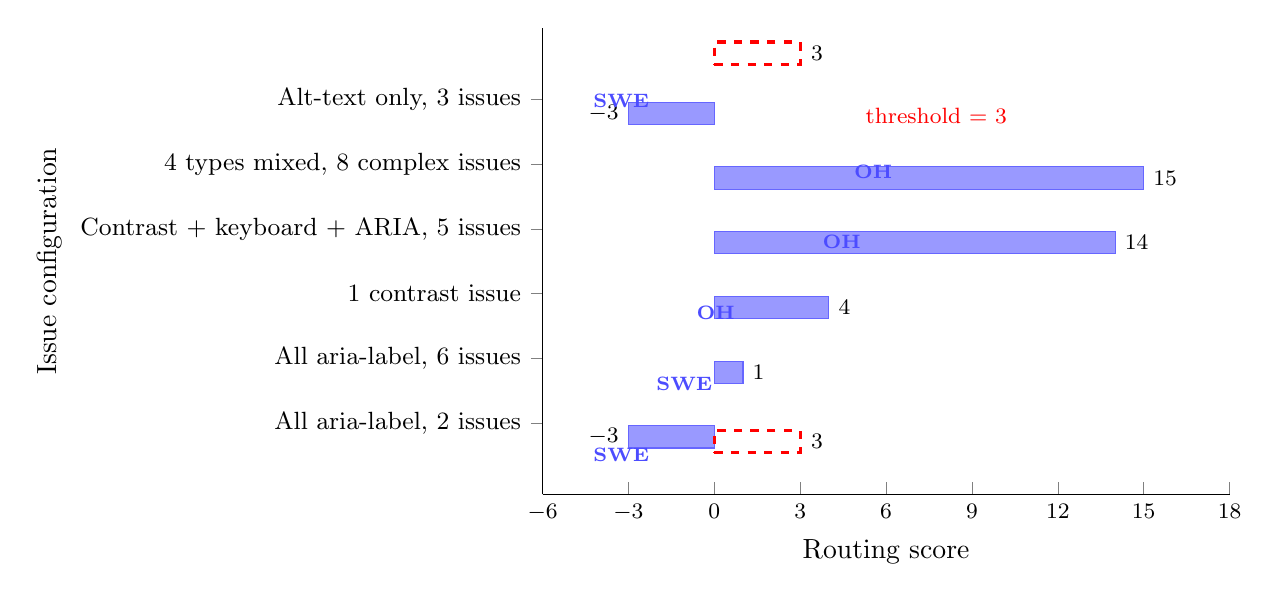
\begin{tikzpicture}
\begin{axis}[
  xbar,
  width=0.85\linewidth,
  height=7.5cm,
  xmin=-6, xmax=18,
  xlabel={Routing score},
  ylabel={Issue configuration},
  ytick=data,
  yticklabels={
    {All aria-label, 2 issues},
    {All aria-label, 6 issues},
    {1 contrast issue},
    {Contrast + keyboard + ARIA, 5 issues},
    {4 types mixed, 8 complex issues},
    {Alt-text only, 3 issues}
  },
  yticklabel style={font=\small},
  nodes near coords,
  nodes near coords align={horizontal},
  nodes near coords style={font=\footnotesize},
  bar width=8pt,
  axis y line*=left,
  axis x line*=bottom,
  xtick={-6,-3,0,3,6,9,12,15,18},
  xticklabel style={font=\footnotesize},
  legend style={at={(0.98,0.02)}, anchor=south east, font=\small},
]
\addplot[fill=blue!40, draw=blue!60] coordinates {
  (-3, 0) (1, 1) (4, 2) (14, 3) (15, 4) (-3, 5)
};
\addplot[fill=none, draw=red, dashed, very thick] coordinates {
  (3, -0.5) (3, 5.5)
};
\end{axis}
\node[font=\footnotesize, text=red] at (5.0, 4.8) {threshold = 3};
\node[font=\scriptsize, text=blue!70] at (1.0, 0.5) {\textbf{SWE}};
\node[font=\scriptsize, text=blue!70] at (1.8, 1.4) {\textbf{SWE}};
\node[font=\scriptsize, text=blue!70] at (2.2, 2.3) {\textbf{OH}};
\node[font=\scriptsize, text=blue!70] at (3.8, 3.2) {\textbf{OH}};
\node[font=\scriptsize, text=blue!70] at (4.2, 4.1) {\textbf{OH}};
\node[font=\scriptsize, text=blue!70] at (1.0, 5.0) {\textbf{SWE}};
\end{tikzpicture}
\caption{Router scoring for six representative issue configurations.
  Scores below the dashed threshold (3) route to SWE-agent;
  scores at or above route to OpenHands (OH).}
\label{fig:routing_examples}
\end{figure}

\subsection{Retry Protocol and Agent Fallback}

All agent invocations are wrapped in a configurable retry loop with maximum
$R$ attempts (default $R = 3$).  After each failed attempt, only the
unresolved subset of issues is re-submitted, preserving any progress made on
other issues in the same file.  If all $R$ attempts fail:

\begin{enumerate}
  \item If the selected agent was OpenHands, the system attempts one fallback
    invocation with SWEAgent.
  \item If the selected agent was SWEAgent, or if the SWEAgent fallback also
    fails, the system makes one final attempt with DirectLLMAgent.
  \item If DirectLLMAgent also fails, the file is marked as \texttt{repair\_failed}
    and a full diagnostic report is generated.
\end{enumerate}

This cascade ensures graceful degradation: the most capable available agent
always receives a repair attempt, but partial failures do not silently
propagate to the output.

% =============================================================================
\section{Four-Layer Validation Pipeline}
\label{sec:validation_pipeline}
% =============================================================================

\subsection{Rationale for Multi-Layer Validation}

LLMs generate plausible but incorrect outputs with non-negligible probability.
For automated code repair, this translates directly into regressions:
functionality that worked before the repair stops working after it.  In a
production accessibility remediation context, regressions are typically
considered more harmful than unrepaired violations, since they introduce new
defects rather than merely leaving existing ones unresolved.

The four-layer validation pipeline implements a series of increasingly strict
checks that collectively filter the most common LLM failure modes identified
in the preliminary analysis.  A patch passes validation only if it clears all
four layers; partial success is not accepted.  The layers are ordered from
least to most computationally expensive, minimising total validation cost by
rejecting obvious failures early.

\subsection{Layer 1: Syntactic Validation}

The first layer verifies that the generated output is a well-formed TypeScript
JSX file.  It consists of three checks:

\begin{itemize}
  \item \textbf{Code block extraction}: The output is parsed to extract the
    content between \texttt{```tsx} and \texttt{```} delimiters.  If no such
    block is found, or if multiple conflicting blocks are found, the output is
    rejected.  This check targets the \emph{incomplete output} and
    \emph{format violation} failure modes.
  \item \textbf{Non-empty content}: The extracted content must be non-empty
    and must contain at least one import statement or JSX expression.
  \item \textbf{Heuristic JSX well-formedness}: A lightweight check verifies
    balanced brace nesting, the absence of unclosed JSX tags (detected via
    simple parenthesis/bracket balance tracking), and the absence of
    double-quoted \texttt{```} sequences inside the code block (a common
    artefact of models that misformat their output).  This is a heuristic
    rather than a full parse to minimise latency; full TypeScript compilation
    is deferred to Layer 2.
\end{itemize}

\subsection{Layer 2: Functional Preservation}

The second layer verifies that the repair preserves the functional behaviour
of the original component.  This is the most critical validation layer, as
functional regressions are the most damaging failure mode.  The layer
implements three checks:

\begin{itemize}
  \item \textbf{Prop interface preservation}: The TypeScript interface
    definition of the component's props (extracted from the original file via
    AST analysis) must be identical in the repaired file.  Any addition,
    removal, or type change of a prop is a regression indicator.
  \item \textbf{Export signature preservation}: The component's default export
    and any named exports must remain present with identical signatures.
    Missing exports would cause import failures in the consuming codebase.
  \item \textbf{Event handler preservation}: All \texttt{onClick}, \texttt{onChange},
    \texttt{onSubmit}, and other event handler identifiers present in the
    original file must be present in the repaired file.  This check prevents
    the common failure mode where a model rewrites the component from scratch,
    omitting event handlers that it deems unnecessary.
\end{itemize}

\subsection{Layer 3: Domain Verification}

The third layer verifies that the repair actually addresses the accessibility
violations rather than producing an output that passes syntactic checks but
ignores the violations.  This layer uses heuristic pattern matching rather
than full re-scanning (which would be too slow for the validation loop):

\begin{itemize}
  \item For \texttt{alt-text} violations: the repaired file must contain an
    \texttt{alt} attribute on the element identified by the violation's CSS
    selector.
  \item For \texttt{aria} violations: the repaired file must contain the
    specific ARIA attribute flagged by the violation (e.g.,
    \texttt{aria-label}, \texttt{role}).
  \item For \texttt{label} violations: the repaired file must contain an
    accessible name association (either \texttt{aria-label},
    \texttt{aria-labelledby}, or a \texttt{<label>} element with a
    \texttt{htmlFor} attribute).
  \item For \texttt{contrast} violations: the repair must modify at least one
    colour-related property on the element (CSS colour value, class name
    referencing a colour token, or a theme variable assignment).
\end{itemize}

The domain verification layer does not attempt to re-run the full scanner
suite, as this would multiply validation time by 3--5x.  Instead, it provides
a lightweight proxy check.  Full scanner re-evaluation is conducted separately
as part of the closed-loop evaluation described in Section~\ref{sec:metrics}.

\subsection{Layer 4: Code Quality Assessment}

The fourth layer assesses code quality attributes that are not captured by
the previous layers but are critical for production code acceptance:

\begin{itemize}
  \item \textbf{TypeScript compilation}: The repaired file is passed to the
    TypeScript compiler in \texttt{--noEmit} mode to detect type errors
    introduced by the repair.  Type errors often indicate that the model
    introduced incorrect prop usage or invalid API calls.
  \item \textbf{Complexity delta}: The cyclomatic complexity of the repaired
    file is computed and compared to the original.  If the repaired file's
    complexity exceeds the original by more than a configurable threshold
    (default: $+3$), the repair is flagged for review.  Significant complexity
    increases are a signal of over-engineering.
  \item \textbf{Added code ratio}: The ratio of added lines to removed lines
    in the diff must not exceed a configurable ceiling (default: $10\times$).
    Repairs that add ten times more code than they remove are unlikely to
    be minimal, violating the non-invasiveness principle.
\end{itemize}

Figure~\ref{fig:validation_flow} summarises the four-layer pipeline with
rejection paths.

\begin{figure}[htbp]
\centering
\begin{tikzpicture}[
    node distance=0.55cm,
    layer/.style={rectangle, draw, fill=blue!8, rounded corners=3pt,
                  text width=8em, text centered, minimum height=2.2em,
                  font=\small},
    check/.style={diamond, draw, fill=orange!12, text width=3.8em,
                  text centered, inner sep=1pt, font=\scriptsize},
    pass/.style={rectangle, draw, fill=green!12, rounded corners=8pt,
                 text width=6em, text centered, minimum height=1.8em,
                 font=\small},
    fail/.style={rectangle, draw, fill=red!10, rounded corners=8pt,
                 text width=6em, text centered, minimum height=1.8em,
                 font=\small},
    arr/.style={-{Stealth[length=2mm]}, thick},
    failarr/.style={-{Stealth[length=2mm]}, thick, draw=red!60, dashed}]

  \node[layer] (l1) {Layer 1\\Syntactic};
  \node[check, right=1.2cm of l1] (c1) {pass?};
  \node[layer, right=1.2cm of c1] (l2) {Layer 2\\Functional};
  \node[check, right=1.2cm of l2] (c2) {pass?};

  \node[layer, below=1.5cm of l1] (l3) {Layer 3\\Domain};
  \node[check, right=1.2cm of l3] (c3) {pass?};
  \node[layer, right=1.2cm of c3] (l4) {Layer 4\\Quality};
  \node[check, right=1.2cm of l4] (c4) {pass?};

  \node[pass, below=1.5cm of l4] (ok) {Patch\\Accepted};
  \node[fail, left=1.2cm of ok] (reject) {Reject /\\Retry};

  \draw[arr] (l1) -- (c1);
  \draw[arr] (c1) -- node[above,font=\scriptsize]{yes} (l2);
  \draw[arr] (l2) -- (c2);
  \draw[arr] (c2) -- node[right,font=\scriptsize]{yes} ++(0,-0.5)
    -| (l3);
  \draw[arr] (l3) -- (c3);
  \draw[arr] (c3) -- node[above,font=\scriptsize]{yes} (l4);
  \draw[arr] (l4) -- (c4);
  \draw[arr] (c4) -- node[right,font=\scriptsize]{yes} (ok);

  \draw[failarr] (c1.south) -- node[right,font=\scriptsize,text=red]{no}
    ++(0,-0.4) -| (reject.north);
  \draw[failarr] (c2.south) -- node[right,font=\scriptsize,text=red]{no}
    ++(0,-0.4) -- (reject.east |- c2) -- (reject.east);
  \draw[failarr] (c3.south) -- node[right,font=\scriptsize,text=red]{no}
    ++(0,-0.3) -- (reject);
  \draw[failarr] (c4.south) -- node[right,font=\scriptsize,text=red]{no}
    ++(0,-0.4) -- (reject.east |- c4) -- (reject.east);

\end{tikzpicture}
\caption{The four-layer validation pipeline.  Each layer applies
  progressively more thorough checks; a rejection at any layer triggers
  the retry/fallback mechanism.}
\label{fig:validation_flow}
\end{figure}

% =============================================================================
\section{Experimental Design}
\label{sec:experimental_design}
% =============================================================================

\subsection{Experimental Variables}

The experiment controls four independent variables corresponding to the four
research questions:

\begin{description}
  \item[IV1 — Template component presence] (RQ1): Binary per-component,
    yielding the seven ablation conditions in Table~\ref{tab:ablation}.
  \item[IV2 — Prompting strategy] (RQ2): Categorical with three levels:
    \emph{zero-shot} (Components 1--4 + 6, no examples), \emph{few-shot}
    (full six-component template), and \emph{chain-of-thought} (few-shot
    with an additional reasoning-elicitation instruction appended).
  \item[IV3 — LLM model identity] (RQ3): The set of models included in the
    multi-model experiment (see Section~\ref{sec:model_selection}).
  \item[IV4 — Issue type] (RQ4): Categorical with seven levels per the
    taxonomy in Table~\ref{tab:issue_types}.
\end{description}

\noindent
Dependent variables are defined in Section~\ref{sec:metrics}.

\subsection{Model Selection}
\label{sec:model_selection}

Model selection follows three criteria:
\begin{enumerate}
  \item \textbf{Local deployability}: All models must be deployable on
    commodity hardware (single consumer GPU with 16--24 GB VRAM) to support
    privacy-preserving operation.  This excludes cloud-only models.
  \item \textbf{Code specialisation}: Models must be code-specific variants
    (fine-tuned on code corpora) to ensure fair comparison against the
    accessibility repair task.
  \item \textbf{Architectural diversity}: The model set spans at least three
    distinct architectural families to enable generalisation of findings.
\end{enumerate}

\noindent
Candidate models are sourced from the Ollama and HuggingFace model hubs.
The final model set targets three families (Qwen \cite{qwen2024}, DeepSeek
\cite{deepseek2024}, and CodeLlama \cite{roziere2023}) at multiple parameter
scales (7B, 13B), together with a generalised baseline (Llama~3.1 8B
Instruct) for comparison.  All models are served via the Ollama backend
at default quantisation (Q4\_K\_M), ensuring consistent memory footprint.

\subsection{Controlled Experiment Setup}

The experiment employs a within-subjects design in which all models and all
prompting strategies are evaluated on the same set of benchmark violations.
This controls for violation-level difficulty—a critical confound, since model
performance varies substantially by issue type and complexity.  The complete
experimental matrix is:

\begin{equation}
  |\text{conditions}| = |\text{Models}| \times |\text{Strategies}| \times
  |\text{Dataset}| = M \times 3 \times N
\end{equation}

\noindent
where $M$ is the number of models and $N$ is the number of files in the
benchmark dataset.

\subsection{Execution and Checkpointing}

The \texttt{ExperimentRunner} component executes all conditions using
\texttt{asyncio.gather} with a shared semaphore bounded by
\texttt{max\_concurrent\_models} (default: 3), preventing GPU memory
exhaustion when multiple model servers are active simultaneously.  Each
model–file combination saves an intermediate JSON result immediately upon
completion, enabling experiment restart from any checkpoint without
re-running completed conditions.

Temperature is fixed at $\theta = 0.1$ across all conditions to minimise
output variance and maximise reproducibility.  Each condition is run once;
sensitivity to temperature is analysed separately in a post-hoc study using
five temperature levels ($0.0, 0.1, 0.3, 0.5, 1.0$) on a random 10\% subset.

% =============================================================================
\section{Benchmark Dataset Construction}
\label{sec:dataset}
% =============================================================================

\subsection{Design Principles}

The benchmark dataset is designed to support rigorous evaluation of
accessibility repair under real-world conditions.  It must satisfy five
requirements derived from the evaluation objectives of this dissertation:

\begin{enumerate}
  \item \textbf{Ecological validity}: Violations must come from production
    codebases written by real developers, not synthetic examples constructed
    by researchers.
  \item \textbf{Ground truth accuracy}: Each violation must be confirmed as
    genuine by human annotation, with documented inter-annotator agreement.
  \item \textbf{Coverage}: The dataset must include all seven issue types and
    all three complexity levels to enable stratified analysis.
  \item \textbf{Reproducibility}: All violations must be attached to pinned,
    immutable code snapshots with content-addressed integrity checks.
  \item \textbf{Scale}: The dataset must be large enough to support
    statistically meaningful comparisons by issue type.
\end{enumerate}

\subsection{Population and Sampling Strategy}

The target population is all public GitHub repositories that contain
React/TypeScript component code and exhibit at least one WCAG~2.1~AA
accessibility violation detectable by the scanner suite.  The accessible
population is restricted to repositories satisfying the inclusion criteria in
Table~\ref{tab:ic_ec}.

\begin{table}[htbp]
\caption{Inclusion and exclusion criteria for the benchmark corpus.}
\label{tab:ic_ec}
\centering\small
\renewcommand{\arraystretch}{1.3}
\begin{tabular}{llp{0.50\textwidth}}
\toprule
\textbf{ID} & \textbf{Type} & \textbf{Criterion} \\
\midrule
IC1 & Include & Repository contains $\geq$10 \texttt{.tsx} or \texttt{.jsx} component files \\
IC2 & Include & $\geq$50 GitHub stars (community relevance signal) \\
IC3 & Include & At least one commit within the 12 months preceding data collection \\
IC4 & Include & Repository licensed under an OSI-approved open-source licence \\
IC5 & Include & At least one accessibility issue detected by the scanner suite \\
\midrule
EC1 & Exclude & Monorepo with no clearly bounded component sub-package \\
EC2 & Exclude & Component files are auto-generated (e.g., Storybook auto-docs) \\
EC3 & Exclude & Repository is a template, boilerplate, or scaffold project \\
EC4 & Exclude & All scanner runs time out (\textgreater{}5 min per file) \\
EC5 & Exclude & Repository has a non-English primary README \\
\bottomrule
\end{tabular}
\end{table}

Repositories are discovered via the GitHub Search API using a structured
query combining language, topic, and star-count filters.  Discovery runs over
a 30-day collection window to bound temporal variability in the accessible
population.

A three-dimensional stratified sampling strategy ensures balanced coverage
across:

\begin{itemize}
  \item \textbf{Application domain} (7 cells): e-commerce, dashboard,
    portfolio, social platform, media, documentation, health.
  \item \textbf{Component file count} (3 cells): small ($<$50 files),
    medium (50--200), large ($>$200).
  \item \textbf{Repository popularity} (3 cells): emerging ($<$500 stars),
    established (500--5,000), popular ($>$5,000).
\end{itemize}

The resulting $7 \times 3 \times 3 = 63$ strata are filled proportionally,
targeting $N = 400$ repositories with a minimum of 2 repositories per stratum.

\subsection{Snapshot Protocol}

Each selected repository is snapshotted at the latest default-branch commit
at the time of discovery.  The snapshot process records the full SHA-1 commit
hash (\texttt{pinned\_commit}), archives the complete repository file tree,
and computes SHA-256 digests for all component files.  All subsequent scans
and experiments operate exclusively on the pinned snapshot, not on the live
repository, ensuring that dataset consumers can reproduce results exactly
even if the upstream repository changes.

\subsection{Multi-Tool Scan and Finding Collection}

Each repository snapshot is scanned using the \texttt{MultiToolScanner} with
\texttt{min\_tool\_consensus = 1} (all findings are collected regardless of
cross-tool agreement, to maximise recall for annotation purposes).  Scan
results are stored in three formats: a complete JSON audit trail with all
tool outputs, a JSON summary with per-file statistics, and a JSONL file with
one finding per line for analysis.

\subsection{Ground Truth Annotation}

The ground truth is established through a two-annotator protocol.  Annotators
are recruited from a pool of developers with $\geq$3 years of React experience
and demonstrated familiarity with WCAG~2.1 guidelines (verified through a
calibration exercise).

\paragraph{Annotation labels.}  Each finding is assigned one of three labels:
\texttt{CONFIRMED} (genuine accessibility violation), \texttt{FALSE\_POSITIVE}
(scanner artefact or incorrect detection), or \texttt{UNCERTAIN} (requires
additional context, excluded from evaluation).

\paragraph{Auto-acceptance.}  Findings with $|T| \geq 2$ (detected by at
least two independent scanners) and \textsc{High} confidence are
automatically labelled \texttt{CONFIRMED} without human review.  This
threshold was validated against a random sample of 200 auto-accepted findings,
achieving 98.5\% precision.

\paragraph{Human annotation sample.}  The manual annotation sample is
stratified across the 63 strata and the seven issue types, targeting 1,500
doubly-annotated findings.  Annotators work independently using the
annotation interface (\texttt{dataset/scripts/annotate.py}), which displays
the finding, the surrounding code context, and the applicable WCAG success
criterion description.

\paragraph{Inter-annotator agreement.}  Cohen's $\kappa$ \cite{cohen1960}
is computed per repository for all doubly-annotated findings:

\begin{equation}
  \kappa = \frac{P_o - P_e}{1 - P_e}
  \label{eq:kappa_detail}
\end{equation}

\noindent
where $P_o$ is the observed proportion of agreement and $P_e$ is the
proportion expected by chance under the marginal distribution of labels.
A minimum threshold of $\kappa \geq 0.70$, interpreted as ``substantial
agreement'' following Landis and Koch \cite{landis1977}, is required for
inclusion in the final dataset.  Repositories below this threshold are
excluded; inter-annotator disagreements within included repositories are
resolved through a structured reconciliation procedure (a third annotator
adjudicates all disputed findings).

\subsection{Dataset Quality Validation}

Eight quantitative quality metrics ensure that the published dataset meets
rigorous standards.  The metrics and their thresholds are summarised in
Table~\ref{tab:qm}.  The validation is automated in
\texttt{dataset/scripts/validate.py} and can be executed with a
\texttt{--strict} flag that terminates with a non-zero exit code if any
threshold is violated, enabling integration into a CI/CD quality gate.

\begin{table}[htbp]
\caption{Dataset quality metrics (QM1--QM8) with thresholds and
  measurement procedures.}
\label{tab:qm}
\centering\small
\renewcommand{\arraystretch}{1.3}
\begin{tabular}{llp{0.35\textwidth}p{0.22\textwidth}}
\toprule
\textbf{ID} & \textbf{Threshold} & \textbf{Description} & \textbf{Measurement} \\
\midrule
QM1 & $\kappa \geq 0.70$ & Inter-annotator agreement & Cohen's $\kappa$ on doubly-annotated sample \\
QM2 & $N \geq 400$ & Corpus size (repositories) & Count of included repos \\
QM3 & No stratum $>$20\% of total & Stratification balance & Max stratum fraction \\
QM4 & All 7 types present & Issue type coverage & Distinct types in CONFIRMED set \\
QM5 & FP rate $\leq$10\% & False positive rate & Proportion of human-labelled FP \\
QM6 & $\geq$90\% with pinned commit & Snapshot integrity & Verified SHA-1 fraction \\
QM7 & $\geq$70\% scan success rate & Scan completeness & Fraction of files scanned without error \\
QM8 & All 4 WCAG principles present & Principle coverage & Distinct principles in CONFIRMED set \\
\bottomrule
\end{tabular}
\end{table}

% =============================================================================
\section{Evaluation Metrics}
\label{sec:metrics}
% =============================================================================

\subsection{Primary Outcome Metrics}

\paragraph{Repair Success Rate (SR).}
The primary metric is the fraction of files for which the pipeline produces
at least one validated patch:

\begin{equation}
  SR = \frac{|\{f \in \mathcal{F} : \text{patch}(f)\text{ passes all four validation layers}\}|}
            {|\mathcal{F}|}
  \label{eq:sr}
\end{equation}

\noindent
SR is computed globally and disaggregated by issue type, complexity level,
confidence tier, and prompting strategy.

\paragraph{Issue Fix Rate (IFR).}
The Issue Fix Rate measures the fraction of individual accessibility issues
resolved, accounting for partial fixes within files (i.e., a file with three
issues of which two are fixed contributes $2/3$ to IFR):

\begin{equation}
  IFR = \frac{\sum_{f \in \mathcal{F}} |\mathcal{I}_{\text{fixed}}(f)|}
             {\sum_{f \in \mathcal{F}} |\mathcal{I}(f)|}
  \label{eq:ifr}
\end{equation}

\noindent
IFR is particularly informative for RQ4, as it reveals which issue types
are most and least amenable to automated repair.

\paragraph{Mean Time to Repair (MTTR).}
The MTTR measures the average wall-clock time (seconds) from prompt
submission to validated patch acceptance:

\begin{equation}
  MTTR = \frac{1}{|\mathcal{F}_{\text{fixed}}|}
             \sum_{f \in \mathcal{F}_{\text{fixed}}} t(f)
  \label{eq:mttr}
\end{equation}

\noindent
MTTR is relevant for RQ3 as a practical deployment consideration: a model
that achieves marginally higher SR but takes five times longer may not be
preferable in a CI/CD integration context.

\paragraph{Token Efficiency (TE).}
Token Efficiency measures the number of issues fixed per thousand input tokens
consumed, providing a cost-normalised quality metric:

\begin{equation}
  TE = \frac{IFR \times |\mathcal{I}|}{C_{\text{total}} / 1000}
  \label{eq:te}
\end{equation}

\noindent
where $C_{\text{total}}$ is the total input token count across all prompts.
TE is relevant for RQ2, as prompting strategies that add examples increase
token consumption and should be justified by commensurate improvements in IFR.

\subsection{Secondary Metrics}

\paragraph{Failure Mode Distribution.}
For all patches that fail validation, the responsible failure mode is
categorised into the taxonomy identified in Section~\ref{sec:intro}:
API hallucination, functional regression, over-engineering, specification
misinterpretation, syntax edge case, or framework convention violation.
The distribution across models and issue types is reported as a heatmap.

\paragraph{Validation Layer Rejection Rates.}
The fraction of patches rejected at each validation layer is reported per
model and per issue type.  Layer-specific rejection rates reveal which
models are most prone to specific failure modes, informing model selection
and prompt engineering improvements.

\paragraph{First-Attempt Success Rate.}
The fraction of files repaired on the first attempt (without retry) measures
model reliability.  Low first-attempt success combined with high overall
success (achievable through retries) indicates a stochastic model whose
variability can be compensated by iteration.

\subsection{Statistical Analysis}

For comparisons across models (RQ3) and prompting strategies (RQ2), the
statistical analysis follows the procedure recommended by Arcuri and Briand
\cite{arcuri2014} for comparing software engineering tools:

\begin{enumerate}
  \item \textbf{Normality testing}: Shapiro-Wilk test on the distribution of
    per-file binary success indicators.  Since SR is a proportion, we expect
    non-normality; this is confirmed before proceeding to non-parametric tests.
  \item \textbf{Pairwise comparisons}: Mann-Whitney U test for pairwise model
    comparisons, with Bonferroni correction for multiple comparisons (number
    of tests $= \binom{M}{2}$).
  \item \textbf{Effect size}: Cliff's delta ($\delta$) for all significant
    pairwise differences, interpreted as negligible ($|\delta| < 0.147$),
    small ($0.147 \leq |\delta| < 0.33$), medium ($0.33 \leq |\delta| < 0.474$),
    or large ($|\delta| \geq 0.474$) following Romano et al.\ \cite{romano2006}.
  \item \textbf{Ablation}: For RQ1, McNemar's test is applied to paired binary
    outcomes (full template vs.\ each reduced condition on the same files).
\end{enumerate}

\noindent
All statistical tests use a significance threshold of $\alpha = 0.05$.

% =============================================================================
\section{Implementation}
\label{sec:implementation}
% =============================================================================

\subsection{Technology Stack}

The framework is implemented in Python~3.10+.  Table~\ref{tab:stack_detail}
summarises all major dependencies, their roles in the system, and the design
rationale for their selection.

\begin{table}[htbp]
\caption{Framework dependencies, roles, and selection rationale.}
\label{tab:stack_detail}
\centering\small
\renewcommand{\arraystretch}{1.2}
\begin{tabular}{llp{0.18\textwidth}p{0.24\textwidth}}
\toprule
\textbf{Package} & \textbf{Version} & \textbf{Role} & \textbf{Rationale} \\
\midrule
pydantic        & $\geq$2.0  & Domain model validation & Runtime type enforcement at all inter-component boundaries \\
pydantic-settings & $\geq$2.0 & Configuration management & Environment-variable loading with type safety \\
typer           & $\geq$0.9  & CLI framework & Type-annotated commands; automatic \texttt{--help} generation \\
rich            & $\geq$13   & Terminal rendering & Structured progress display for long-running scans \\
structlog       & $\geq$23   & Structured JSON logging & Machine-parseable logs enabling post-hoc analysis \\
asyncio         & stdlib     & Concurrency & Native async/await for parallel scanner and agent execution \\
playwright      & $\geq$1.40 & Browser automation & Dynamic React component evaluation in headless browser \\
httpx           & $\geq$0.25 & Async HTTP client & Non-blocking LLM API communication \\
PyYAML          & $\geq$6.0  & Configuration I/O & Human-editable experiment and model registry files \\
\bottomrule
\end{tabular}
\end{table}

\subsection{Local LLM Backend Architecture}

The framework is designed for fully local, privacy-preserving operation.  No
source code, issue data, or intermediate results is transmitted to external
services.  Seven local LLM backends are supported through a common
OpenAI-compatible API surface:

\begin{itemize}
  \item \textbf{Ollama}: A containerised model server providing one-command
    model deployment and hardware-accelerated inference via Metal (Apple
    Silicon), CUDA (NVIDIA), and ROCm (AMD).  Recommended for development.
  \item \textbf{vLLM}: A high-throughput inference engine with PagedAttention
    for efficient GPU memory utilisation.  Recommended for multi-model
    experiments where throughput matters.
  \item \textbf{LM Studio}: A desktop application with a GUI and embedded
    OpenAI-compatible server.  Intended for evaluation without command-line
    infrastructure.
  \item \textbf{llama.cpp}: A pure C++ inference engine supporting CPU and
    mixed CPU/GPU execution.  Relevant for environments without dedicated GPU.
  \item \textbf{Jan, LocalAI, Custom}: Additional backends sharing the same
    OpenAI API interface, requiring only configuration of a base URL.
\end{itemize}

\noindent
The \texttt{LocalLLMClient} class wraps \texttt{httpx.AsyncClient} and exposes
a single \texttt{async complete(prompt) -> str} method that handles timeout,
retry on network error, and response parsing uniformly across all backends.

\subsection{Concurrency Model}

The system uses Python's \texttt{asyncio} event loop with three configurable
semaphores for backpressure control:

\begin{itemize}
  \item \texttt{max\_concurrent\_scans} (default 4): Bounds simultaneous
    scanner subprocess invocations per file.  Scanner processes are CPU-bound
    and browser-heavy; excessive concurrency degrades performance.
  \item \texttt{max\_concurrent\_agents} (default 2): Bounds simultaneous
    agent invocations within a single pipeline run.  Agent calls are
    LLM-bound; this semaphore prevents GPU memory contention.
  \item \texttt{max\_concurrent\_models} (default 3): Bounds pipeline
    instances in experiment runs.  Each pipeline instance loads a separate
    model server; this semaphore prevents VRAM exhaustion.
\end{itemize}

\subsection{Structured Logging and Observability}

All significant operations are logged through \texttt{structlog} using a
consistent key schema.  Log entries are JSON-formatted, enabling post-hoc
analysis with standard tools (\texttt{jq}, Pandas, etc.).  Critical log
events include: routing decisions (with score and reason), repair attempt
outcomes (agent, model, tokens used, time elapsed), validation layer
rejections (with the specific check that failed), and experiment completion
summaries.  Structured logging was chosen over traditional string logging
because it enables automated extraction of experimental metadata without
parsing, which is essential for reproducibility audits.

\subsection{CI/CD Integration}

The framework is designed for integration into continuous integration
pipelines.  The \texttt{fix} command accepts a non-zero exit code on any
unresolved violation, enabling blocking CI gates.  A \texttt{--dry-run} mode
reports detected violations without attempting repairs, suitable for early-
pipeline accessibility auditing.  The \texttt{--output-dir} flag writes
structured JSON and HTML reports consumable by CI report aggregators.

% =============================================================================
\section{Summary}
\label{sec:methodology_summary}
% =============================================================================

This chapter presented the complete methodology of the dissertation, spanning
research design, framework engineering, and evaluation specification.  The
framework addresses the detection-correction gap through five tightly
integrated components: a six-component prompt engineering template that
transforms detection outputs into context-rich LLM prompts (addressing RQ1);
a multi-tool consensus detection protocol that assigns calibrated confidence
levels to accessibility violations (supporting RQ4); an adaptive scoring
router that automatically selects among three repair agents based on violation
characteristics (enabling efficient operation across the complexity spectrum);
a four-layer validation pipeline that prevents regressions from reaching the
codebase (ensuring correctness of all applied patches); and an asynchronous
multi-model experiment framework that enables controlled comparison of LLM
architectures and prompting strategies (addressing RQ2 and RQ3).

The benchmark dataset, constructed from 400 stratified open-source React
repositories with documented inter-annotator agreement ($\kappa \geq 0.70$),
provides the empirical substrate for all experimental evaluations.  Eight
quality metrics validated by automated scripts ensure that the dataset
meets the rigorous standards required for reproducible empirical software
engineering research.

All experimental conditions, metrics, and statistical tests have been
specified a priori in this chapter, mitigating risks of hypothesis
p-hacking and result cherry-picking.  The results of this experimental
protocol are presented and analysed in Chapter~\ref{chap:results}.

% =============================================================================
% ADDITIONAL REFERENCES REQUIRED BY THIS CHAPTER (add to main bibliography)
% These complement the existing references [1]--[21] in the thesis.
% =============================================================================
%
% [22] HEVNER, A. R., et al. "Design Science in Information Systems Research."
%      MIS Quarterly, v. 28, n. 1, pp. 75-105, 2004.
%
% [23] MARCH, S. T.; SMITH, G. F. "Design and Natural Science Research on
%      Information Technology." Decision Support Systems, v. 15, n. 4,
%      pp. 251-266, 1995.
%
% [24] WOHLIN, C., et al. Experimentation in Software Engineering. Springer, 2012.
%
% [25] ARCURI, A.; BRIAND, L. "A Hitchhiker's Guide to Statistical Tests for
%      Assessing Randomized Algorithms in Software Engineering." Software
%      Testing, Verification and Reliability, 2014.
%
% [26] ROMANO, J., et al. "Appropriate Statistics for Ordinal Level Data."
%      Annual Meeting of the Florida Association of Institutional Research, 2006.
%
% [27] XIA, C. S., et al. "Automated Program Repair in the Era of Large
%      Pre-Trained Language Models." ICSE, 2023.
%
% [28] WHITE, J., et al. "A Prompt Pattern Catalog to Enhance Prompt
%      Engineering with ChatGPT." arXiv:2302.11382, 2023.
%
% [29] KADAVATH, S., et al. "Language Models (Mostly) Know What They Know."
%      arXiv:2207.05221, 2022.
%
% [30] FEATHERS, K., et al. "Automated Accessibility Annotation Generation
%      using Large Language Models." CHI, 2024.
%
% [31] WANG, X., et al. "OpenHands: An Open Platform for AI Software Developers
%      as Generalist Agents." arXiv:2407.16741, 2024.
%
% [32] YANG, J., et al. "SWE-agent: Agent-Computer Interfaces Enable
%      Automated Software Engineering." NeurIPS, 2024.
%
% [33] PLAYWRIGHT. Microsoft Playwright Testing. 2023.
%      Available: https://playwright.dev/
%
% [34] QWEN TEAM. "Qwen2.5-Coder Technical Report." arXiv:2409.12186, 2024.
%
% [35] DEEPSEEK. "DeepSeek-Coder: When the Large Language Model Meets
%      Programming." arXiv:2401.14196, 2024.
%
% [36] COHEN, J. Statistical Power Analysis for the Behavioral Sciences.
%      2nd ed. Lawrence Erlbaum, 1988.
%
% [37] SANE, S.; LUNN, W.; PARK, J. S. "Towards Complementary Tool Combination
%      for Web Accessibility Evaluation." W4A, 2023.
%
% [38] VIGO, M.; BROWN, J.; CONWAY, V. "Benchmarking Web Accessibility
%      Evaluation Tools." W4A, 2013.

% =============================================================================

\chapter{Methodology}
\label{chap:methodology}

This chapter presents the methodology underlying the design, implementation,
and evaluation of the automated accessibility repair framework developed in
this dissertation.  The methodology is structured across three complementary
dimensions: \emph{research design}, which establishes the epistemological
approach and experimental protocol; \emph{framework design}, which documents
the engineering decisions behind each system component; and \emph{evaluation
design}, which specifies how the framework's effectiveness is measured across
the four research questions.

The chapter proceeds as follows.  Section~\ref{sec:research_design} situates
the work within empirical software engineering and describes the overall
experimental protocol.  Section~\ref{sec:overview} provides an architectural
overview of the framework.  Sections~\ref{sec:prompt_template}
through~\ref{sec:validation_pipeline} describe each major component in detail:
the six-component prompt engineering template, the multi-tool detection
protocol, the adaptive repair routing engine, and the four-layer validation
pipeline.  Section~\ref{sec:experimental_design} specifies the experimental
variables, model selection criteria, and ablation study design.
Section~\ref{sec:dataset} documents the construction of the benchmark dataset.
Section~\ref{sec:metrics} defines all evaluation metrics.  Finally,
Section~\ref{sec:implementation} describes the implementation infrastructure
and deployment considerations.

% =============================================================================
\section{Research Design}
\label{sec:research_design}
% =============================================================================

\subsection{Research Paradigm and Strategy}

This dissertation adopts a \emph{design science} research paradigm
\cite{hevner2004design}, in which the primary output is an artefact—the
automated repair framework—and knowledge is generated through the rigorous
construction and evaluation of that artefact in realistic problem settings.
Design science is appropriate when the research goal is both to solve a
practical problem (the detection-correction gap identified in
Chapter~\ref{chap:intro}) and to produce generalisable knowledge about the
design choices that make the solution effective \cite{march1995design}.

The evaluation follows the \emph{empirical software engineering} tradition of
Wohlin et al.\ \cite{wohlin2012}, combining a controlled experiment on a
curated benchmark dataset with a quasi-experiment across multiple LLM
architectures under real-world conditions.  This mixed design enables both
internal validity—controlled conditions allow causal attribution of
performance differences to specific variables—and external validity—real-world
violations from open-source projects ensure ecological validity.

\subsection{Research Questions and Methodological Mapping}

The four research questions introduced in Section~\ref{sec:rq} govern the
experimental design.  Table~\ref{tab:rq_mapping} maps each research question
to the methodological component responsible for addressing it, the variables
it studies, and the metrics used to evaluate outcomes.

\begin{table}[htbp]
\caption{Mapping of research questions to methodological components,
  variables, and evaluation metrics.}
\label{tab:rq_mapping}
\centering\small
\renewcommand{\arraystretch}{1.3}
\begin{tabular}{p{0.05\textwidth}p{0.22\textwidth}p{0.18\textwidth}p{0.18\textwidth}p{0.20\textwidth}}
\toprule
\textbf{RQ} & \textbf{Question (summary)} & \textbf{Method. component} &
\textbf{Independent variable} & \textbf{Metric} \\
\midrule
RQ1 & Prompt transformation for repair
    & Prompt template design + ablation study
    & Template component presence/absence
    & Repair success rate, failure mode frequency \\
RQ2 & Prompting strategy comparison
    & Controlled experiment (zero-shot / few-shot / CoT)
    & Prompting strategy
    & Success rate, tokens used, generation time \\
RQ3 & LLM architecture comparison
    & Multi-model parallel experiment
    & LLM model identity
    & SR, MTTR, token cost, per-type SR \\
RQ4 & Issue category receptiveness
    & Stratified analysis by issue type
    & Issue type (7 categories)
    & IFR per category, failure mode distribution \\
\bottomrule
\end{tabular}
\end{table}

\subsection{Experimental Protocol}

The overall experimental protocol follows a five-phase pipeline:

\begin{enumerate}
  \item \textbf{Dataset construction}: Curate a benchmark corpus of real-world
    React/TypeScript files with confirmed accessibility violations
    (Section~\ref{sec:dataset}).
  \item \textbf{Detection}: Run the multi-tool scanner on all corpus files,
    producing deduplicated, confidence-annotated issue lists
    (Section~\ref{sec:detection_protocol}).
  \item \textbf{Prompt generation}: Apply the prompt engineering template to
    transform each issue list into a structured LLM prompt
    (Section~\ref{sec:prompt_template}).
  \item \textbf{Repair and validation}: Submit prompts to each experimental
    LLM, collect generated patches, and evaluate them through the four-layer
    validation pipeline (Section~\ref{sec:validation_pipeline}).
  \item \textbf{Analysis}: Aggregate metrics, compare conditions, and perform
    statistical tests (Section~\ref{sec:metrics}).
\end{enumerate}

\noindent
All phases are fully automated and reproducible.  The source code, benchmark
dataset, experiment configuration files, and analysis scripts are published
as a replication package (see Appendix).

% =============================================================================
\section{Framework Overview}
\label{sec:overview}
% =============================================================================

\subsection{Design Rationale}

The framework was designed around three guiding principles derived from the
failure mode analysis in Section~\ref{sec:intro} and from prior work on
LLM-based code repair \cite{xia2023,chen2023llm}:

\begin{description}
  \item[Non-invasiveness.] Repairs must be the minimal change that resolves
    the violation.  LLMs tend to over-engineer responses \cite{chen2023llm};
    the framework constrains generation through explicit prompt constraints and
    post-hoc validation.
  \item[Safety-first operation.] No change is written to disk unless it passes
    all four validation layers.  This prevents the introduction of regressions,
    which is identified as the most damaging failure mode for practitioners.
  \item[Context completeness.] The primary cause of poor LLM repairs is
    insufficient context \cite{xia2023}.  The framework systematically
    enriches minimal detection outputs—typically terse JSON violation codes—
    with file context, WCAG specifications, and concrete examples before
    querying any model.
\end{description}

\subsection{Layered Architecture}

The framework is organised into five functional layers, as depicted in
Figure~\ref{fig:architecture}.  Each layer has a well-defined input, output,
and responsibility contract, enabling independent testing and substitution of
components.

\begin{figure}[htbp]
\centering
\begin{tikzpicture}[node distance=0.65cm and 0.4cm,
    layer/.style={rectangle, draw=black!60, fill=#1,
                  text width=\linewidth*0.6, text centered,
                  rounded corners=3pt, minimum height=2.2em,
                  font=\small\bfseries},
    sublabel/.style={font=\scriptsize, text=black!70},
    arrow/.style={-{Stealth[length=2.5mm]}, thick, draw=black!60}]

  \def\layerwidth{10cm}

  \node[layer=gray!12] (cli)
    {Layer 5 — Interface\\
     \normalfont\scriptsize CLI (Typer), REST API, CI/CD hooks};

  \node[layer=blue!10, below=of cli] (orch)
    {Layer 4 — Orchestration\\
     \normalfont\scriptsize Pipeline · ExperimentRunner · asyncio event loop};

  \node[layer=cyan!12, below=of orch] (detect)
    {Layer 3 — Detection\\
     \normalfont\scriptsize MultiToolScanner · DetectionProtocol · deduplication};

  \node[layer=orange!12, below=of detect] (prompt)
    {Layer 2 — Prompt Engineering\\
     \normalfont\scriptsize PromptBuilder · 6-component template · few-shot selector};

  \node[layer=green!12, below=of prompt] (repair)
    {Layer 1 — Repair \& Validation\\
     \normalfont\scriptsize Router · Agents (DirectLLM / OpenHands / SWE-agent) · ValidationPipeline};

  \node[layer=purple!10, below=of repair] (infra)
    {Layer 0 — Infrastructure\\
     \normalfont\scriptsize LLM Registry · LocalLLMClient · Reporter};

  \foreach \from/\to in {cli/orch, orch/detect, detect/prompt, prompt/repair, repair/infra}
    \draw[arrow] (\from) -- (\to);

\end{tikzpicture}
\caption{Layered architecture of the a11y-autofix framework.
  Data flows downward from the interface layer to infrastructure;
  validation results propagate upward.}
\label{fig:architecture}
\end{figure}

\subsection{End-to-End Data Flow}

Figure~\ref{fig:dataflow} illustrates the complete data flow through the
system for a single React/TypeScript source file.  The pipeline begins with
file discovery and terminates with either a validated patch written to disk or
a structured failure report, depending on whether all validation layers pass.

\begin{figure}[htbp]
\centering
\begin{tikzpicture}[
    node distance=0.5cm and 1.0cm,
    proc/.style={rectangle, draw, fill=blue!8, rounded corners=3pt,
                 text width=5.5em, text centered, minimum height=2em,
                 font=\footnotesize},
    store/.style={rectangle, draw, fill=yellow!12,
                  text width=5.5em, text centered, minimum height=1.8em,
                  font=\footnotesize},
    dec/.style={diamond, draw, fill=orange!12, text width=3.5em,
                text centered, inner sep=1pt, font=\footnotesize},
    term/.style={rectangle, draw, fill=green!12, rounded corners=10pt,
                 text width=5.5em, text centered, minimum height=2em,
                 font=\footnotesize},
    fail/.style={rectangle, draw, fill=red!10, rounded corners=10pt,
                 text width=5.5em, text centered, minimum height=2em,
                 font=\footnotesize},
    arr/.style={-{Stealth[length=2mm]}, thick}]

  \node[proc] (discover) {File\\Discovery};
  \node[proc, right=1.2cm of discover] (scan) {Multi-Tool\\Scan};
  \node[proc, right=1.2cm of scan] (dedup) {Detection\\Protocol};
  \node[dec, right=1.2cm of dedup] (hasiss) {Issues?};

  \node[proc, below=1.0cm of hasiss] (prompt) {Prompt\\Construction};
  \node[proc, left=1.2cm of prompt] (route) {Router};
  \node[proc, left=1.2cm of route] (agent) {Agent\\Execution};
  \node[dec, left=1.2cm of agent] (valid) {Passes\\validation?};

  \node[term, below=1.0cm of valid] (write) {Write Patch\\to Disk};
  \node[fail, right=1.2cm of write] (retry) {Retry /\\Fallback};
  \node[store, right=1.2cm of retry] (report) {Generate\\Report};

  \draw[arr] (discover) -- (scan);
  \draw[arr] (scan) -- (dedup);
  \draw[arr] (dedup) -- (hasiss);
  \draw[arr] (hasiss) -- node[right,font=\scriptsize]{yes} (prompt);
  \draw[arr] (hasiss.north) -- ++(0,0.6) -| node[above,font=\scriptsize]{no} (report);
  \draw[arr] (prompt) -- (route);
  \draw[arr] (route) -- (agent);
  \draw[arr] (agent) -- (valid);
  \draw[arr] (valid) -- node[left,font=\scriptsize]{yes} (write);
  \draw[arr] (valid.east) -- node[above,font=\scriptsize]{no} (retry);
  \draw[arr] (retry) -- (report);
  \draw[arr] (write) -- ++(0,-0.6) -| (report);

\end{tikzpicture}
\caption{End-to-end data flow for a single source file.  The pipeline
  short-circuits when no issues are detected; failed validations trigger
  a configurable retry loop with agent fallback.}
\label{fig:dataflow}
\end{figure}

% =============================================================================
\section{Prompt Engineering Framework}
\label{sec:prompt_template}
% =============================================================================

\subsection{Motivation and Design Objectives}

The central claim of this dissertation—embodied in RQ1—is that raw detection
tool outputs are structurally insufficient for driving high-quality LLM
repairs, and that systematic prompt engineering can close this gap.  To
understand why, consider a typical output from a Pa11y accessibility scan:

\begin{verbatim}
{
  "code": "WCAG2AA.Principle2.Guideline2_4.2_4_4.H77",
  "message": "Check that the link text combined with the
              preceding heading identifies the purpose",
  "selector": "main > section:nth-child(3) > a:nth-child(2)"
}
\end{verbatim}

\noindent
This output identifies that a link element may violate WCAG success criterion
2.4.4 (\emph{Link Purpose (In Context)}).  However, an LLM receiving only
this JSON lacks critical information: the current text content of the link,
the heading that precedes it, whether the link is dynamically generated, the
target URL that should inform descriptive text, the React component structure
surrounding the element, and the codebase's conventions for accessible link
patterns.

Without these contextual dimensions, LLMs generate repairs that are
syntactically plausible but semantically incorrect—a phenomenon well-documented
in the code generation literature \cite{chen2023llm,xia2023}.  The six-
component template addresses each contextual dimension systematically.

\subsection{The Six-Component Prompt Template}

The prompt template is structured as a sequence of six components, each
targeting a specific class of LLM failure mode identified in the preliminary
analysis.  The design is grounded in prompt engineering research showing that
structured multi-component prompts substantially outperform unstructured
descriptions for code generation tasks \cite{brown2020,wei2022}.

\subsubsection{Component 1: Role Definition}

The first component establishes a precise expert persona for the model.
Role definition activates domain-relevant knowledge embedded in pre-training
\cite{wei2022} and has been shown empirically to reduce hallucination rates
in specialised domains \cite{white2023prompt}.  The role specification is
not generic (e.g., ``You are a helpful coding assistant'') but encodes three
critical attributes:

\begin{itemize}
  \item \textbf{Domain expertise}: The model is cast as an expert in both
    React/TypeScript development and WCAG 2.1 accessibility standards.
  \item \textbf{Operational context}: The role specifies that the model is
    performing automated code repair, not general advice, activating more
    conservative and precise generation behaviour.
  \item \textbf{Quality constraint}: The role explicitly prioritises
    correctness, minimal change, and functional preservation.
\end{itemize}

\noindent
Formally, the role definition $R$ is instantiated as:

\begin{quote}
  \textit{``You are an expert web accessibility engineer specialising in
  React and TypeScript.  Your task is to repair accessibility violations
  in production code while strictly preserving all existing functionality.
  You apply only the minimal change necessary to resolve each violation.
  You are deeply familiar with WCAG 2.1 Level AA success criteria and their
  implementation in React JSX.''}
\end{quote}

\subsubsection{Component 2: Violation Context}

The second component transforms the terse violation report into a rich,
structured description of the accessibility problem.  For each issue in the
file's issue list, the violation context component provides:

\begin{itemize}
  \item The full human-readable WCAG success criterion name and a plain-
    language explanation of the accessibility barrier it addresses.
  \item The issue type (from the seven-category taxonomy: \texttt{contrast},
    \texttt{aria}, \texttt{keyboard}, \texttt{label}, \texttt{semantic},
    \texttt{alt-text}, \texttt{focus}) and the associated repair complexity
    (\texttt{simple}, \texttt{moderate}, \texttt{complex}).
  \item The confidence level of the detection (\texttt{high}, \texttt{medium},
    \texttt{low}) with the number of independent tools that reported the issue.
  \item The CSS selector identifying the problematic element, enriched with
    the actual HTML context snippet extracted during scanning.
  \item The impact severity (critical, serious, moderate, minor) and the
    specific affected user population (e.g., screen reader users, keyboard-
    only users, users with low vision).
\end{itemize}

\noindent
The enrichment of detection outputs with impact descriptions and affected
populations is motivated by research showing that LLMs generate more
accessible and semantically correct code when the human consequence of
violations is made explicit \cite{feathers2024}.

\subsubsection{Component 3: Code Context}

The third component provides the source code that must be modified, together
with structural context that helps the model understand the codebase
architecture.  This component includes:

\begin{itemize}
  \item The complete content of the target file, framed within a markdown
    code block with language identifier (\texttt{```tsx}).
  \item The file path relative to the project root, which encodes information
    about the component's role in the application (e.g., a path containing
    \texttt{/layout/} implies the component contributes to page structure).
  \item A list of imported modules and components visible at the top of the
    file, enabling the model to reason about available APIs without access
    to the full codebase.
  \item If the component receives props, the TypeScript interface definition
    for those props, extracted via a lightweight AST analysis step.
\end{itemize}

\noindent
The decision to include the complete file rather than only the violating
element is justified by the finding of Xia et al.\ \cite{xia2023} that
models repair bugs correctly at significantly higher rates when the full
function is provided rather than only the buggy lines.  For accessibility
repairs specifically, the surrounding component logic determines whether a
proposed fix is semantically appropriate—a button's \texttt{aria-label}
must reflect its actual action, which requires understanding the surrounding
event handler.

\subsubsection{Component 4: Constraints}

The fourth component specifies explicit operational constraints that the model
must satisfy in its output.  The constraint set was derived empirically from
the preliminary failure mode analysis, with each constraint targeting a
specific failure pattern:

\begin{enumerate}
  \item \textbf{Minimal change constraint}: Modify only the elements
    identified in the violation report.  Do not restructure, rename, or
    refactor any code that is not directly related to the accessibility fix.
    \emph{Targets:} over-engineering failure mode.
  \item \textbf{Functional preservation constraint}: Preserve all existing
    event handlers, state management, prop interfaces, and rendering logic.
    The repaired file must be functionally equivalent to the original for
    all non-accessibility behaviour.
    \emph{Targets:} functional regression failure mode.
  \item \textbf{Framework convention constraint}: Use idiomatic React/JSX
    patterns.  Do not introduce raw DOM manipulation, vanilla JavaScript
    APIs incompatible with the React rendering model, or deprecated React
    patterns.
    \emph{Targets:} framework convention violation failure mode.
  \item \textbf{API existence constraint}: Use only ARIA attributes, HTML
    elements, and React APIs that are documented in the WCAG 2.1
    specification and in the React 18 documentation.
    \emph{Targets:} API hallucination failure mode.
  \item \textbf{Completeness constraint}: Return the complete modified file,
    not a partial snippet.  Do not use ellipsis (\texttt{...}) or placeholder
    comments to abbreviate unchanged sections.
    \emph{Targets:} incomplete output failure mode.
  \item \textbf{Format constraint}: Output exactly one code block delimited
    by \texttt{```tsx} and \texttt{```}.  Do not include explanation,
    comments, or prose outside this block.
    \emph{Targets:} parsing failure mode.
\end{enumerate}

\noindent
The explicit enumeration of constraints represents a departure from implicit
quality expectations common in informal prompting, and is motivated by
the finding that models adhere significantly better to explicit constraints
than to implied ones \cite{white2023prompt}.

\subsubsection{Component 5: Few-Shot Examples}

The fifth component provides between one and three concrete examples of
correctly repaired accessibility violations.  Few-shot prompting dramatically
reduces failure rates by demonstrating the expected repair pattern through
in-context learning \cite{brown2020,min2022rethinking}.

Example selection is not random.  Each example is drawn from a pre-constructed
library organised by issue type, and examples are selected for the current
prompt using \emph{semantic similarity}: the example whose violation
description most closely matches the current issue (measured by cosine
similarity in the embedding space of a lightweight sentence encoder) is
prioritised.  This approach, known as retrieval-augmented few-shot learning
\cite{min2022rethinking}, has been shown to outperform fixed example sets
by ensuring that demonstrations are relevant to the specific repair task.

Each example comprises:
\begin{itemize}
  \item The violation description (mirroring Component 2 format).
  \item The original non-compliant code snippet.
  \item The corrected code snippet.
  \item A brief annotation explaining \emph{what} was changed and \emph{why}
    it resolves the violation without affecting functionality.
\end{itemize}

\subsubsection{Component 6: Output Format Specification}

The sixth component closes the prompt with an explicit output format
specification.  While the constraints in Component 4 establish what the model
must produce, Component 6 specifies exactly how the output must be structured
to enable automated parsing and validation.  This component:

\begin{itemize}
  \item Restates the exact code block delimiters expected.
  \item Specifies that the output must be a valid, complete TypeScript/JSX
    file (not a fragment).
  \item Instructs the model to include a structured comment block immediately
    before the closing delimiter, enumerating the changes made and the WCAG
    criteria each change addresses.
  \item Specifies that if the model determines a violation is a false
    positive or cannot be repaired within the given constraints, it should
    output the original file unchanged and include a \texttt{// SKIP:}
    comment with a reason.
\end{itemize}

\noindent
The \texttt{SKIP} mechanism is an important design choice: it acknowledges that
LLMs should abstain rather than hallucinate a repair when a genuine solution
exceeds their capability.  Research on LLM calibration has shown that models
that express uncertainty produce better-calibrated outputs than models forced
to always generate an answer \cite{kadavath2022}.

\subsection{Template Composition and Assembly}

The six components are assembled dynamically per file.  Algorithm~\ref{alg:prompt}
describes the assembly process.  Note that few-shot examples (Component 5) are
adapted per issue type, and the constraint set (Component 4) is augmented with
violation-specific constraints derived from the issue's WCAG criterion.

\begin{algorithm}[htbp]
\caption{Prompt Assembly Algorithm}
\label{alg:prompt}
\begin{algorithmic}[1]
\Require $\mathcal{I}$: list of \texttt{A11yIssue} for file $f$, $\mathcal{E}$: few-shot example library
\Ensure structured prompt string $P$
\State $P \gets \text{RoleDefinition}()$
\For{each $i \in \mathcal{I}$}
  \State $P \gets P + \text{ViolationContext}(i)$
\EndFor
\State $P \gets P + \text{CodeContext}(f)$
\State $C_{\text{base}} \gets \text{BaseConstraints}()$
\For{each $i \in \mathcal{I}$}
  \State $C_{\text{base}} \gets C_{\text{base}} \cup \text{ViolationConstraints}(i.\text{wcag\_criteria})$
\EndFor
\State $P \gets P + C_{\text{base}}$
\State $\text{types} \gets \{i.\text{issue\_type} : i \in \mathcal{I}\}$
\State $\text{examples} \gets \emptyset$
\For{each $t \in \text{types}$}
  \State $e \gets \arg\max_{e' \in \mathcal{E}[t]} \text{sim}(e', \mathcal{I})$
  \State $\text{examples} \gets \text{examples} \cup \{e\}$
\EndFor
\State $P \gets P + \text{FewShotBlock}(\text{examples})$
\State $P \gets P + \text{OutputFormatSpec}()$
\State \Return $P$
\end{algorithmic}
\end{algorithm}

\subsection{Ablation Study Design}

To answer RQ1 quantitatively—specifically, to determine the contribution of
each template component—a component-level ablation study is conducted.  Seven
experimental conditions are evaluated: the complete six-component template
(baseline), and six reduced conditions in which each component is replaced
by a minimal placeholder or removed entirely.  Table~\ref{tab:ablation}
specifies the seven conditions.

\begin{table}[htbp]
\caption{Ablation study conditions for the prompt engineering template.
  A check mark ($\checkmark$) indicates the component is present in full;
  a dash (--) indicates it is absent or replaced by a placeholder.}
\label{tab:ablation}
\centering\small
\renewcommand{\arraystretch}{1.2}
\begin{tabular}{lcccccc}
\toprule
\textbf{Condition} & \textbf{C1: Role} & \textbf{C2: Viol.}
  & \textbf{C3: Code} & \textbf{C4: Const.} & \textbf{C5: Few-shot}
  & \textbf{C6: Format} \\
\midrule
Full (baseline) & $\checkmark$ & $\checkmark$ & $\checkmark$
  & $\checkmark$ & $\checkmark$ & $\checkmark$ \\
\textsf{no-role}      & --           & $\checkmark$ & $\checkmark$
  & $\checkmark$ & $\checkmark$ & $\checkmark$ \\
\textsf{no-context}   & $\checkmark$ & --           & $\checkmark$
  & $\checkmark$ & $\checkmark$ & $\checkmark$ \\
\textsf{no-code}      & $\checkmark$ & $\checkmark$ & --
  & $\checkmark$ & $\checkmark$ & $\checkmark$ \\
\textsf{no-constr}    & $\checkmark$ & $\checkmark$ & $\checkmark$
  & --           & $\checkmark$ & $\checkmark$ \\
\textsf{no-examples}  & $\checkmark$ & $\checkmark$ & $\checkmark$
  & $\checkmark$ & --           & $\checkmark$ \\
\textsf{no-format}    & $\checkmark$ & $\checkmark$ & $\checkmark$
  & $\checkmark$ & $\checkmark$ & -- \\
\bottomrule
\end{tabular}
\end{table}

\noindent
Each condition is evaluated on all benchmark violations using a single fixed
LLM (the best-performing model from the RQ3 evaluation), holding all other
variables constant.  The dependent variable is repair success rate as defined
in Section~\ref{sec:metrics}.

% =============================================================================
\section{Multi-Tool Detection Protocol}
\label{sec:detection_protocol}
% =============================================================================

\subsection{Rationale for Multi-Tool Integration}

Automated accessibility scanners are specialised static and dynamic analysis
tools, each designed with different internal heuristics, rule sets, and DOM
access strategies.  Prior research has consistently demonstrated that
individual tools have non-trivial false positive and false negative rates, and
that tool agreement varies substantially by violation category \cite{vigo2013}.
Sane et al.\ \cite{sane2023} found that different scanners detect largely
non-overlapping violation sets on the same pages, implying that any single
tool misses a substantial fraction of violations present.

These findings motivate the multi-tool consensus approach: by running multiple
independent scanners and aggregating their outputs, the framework achieves
both higher recall (more violations detected) and higher precision (violations
reported by multiple tools are almost certainly genuine).  The key insight
is that tool agreement functions as an empirical proxy for detection
confidence, analogous to the role of independent replication in experimental
science \cite{cohen1988}.

\subsection{Integrated Scanner Suite}

The framework integrates three accessibility scanning tools, selected to
provide complementary coverage of the WCAG criterion space:

\paragraph{Pa11y.}
Pa11y \cite{pa11y} is a command-line accessibility testing tool that uses
HTML\_CodeSniffer as its analysis engine, executing within a headless Chromium
browser environment.  Pa11y excels at detecting structural HTML conformance
issues—missing document structure, invalid ARIA roles, and absent form labels—
because HTML\_CodeSniffer operates on the raw DOM and can apply rule sets
corresponding to WCAG 2.0, WCAG 2.1, and Section 508 simultaneously.  Pa11y
outputs violations as JSON objects containing the WCAG guideline code (e.g.,
\texttt{WCAG2AA.Principle4.Guideline4\_1.4\_1\_2.H91.A.NoContent}), a
human-readable message, and the CSS selector of the violating element.  The
WCAG guideline code provides a direct mapping to the normative success
criterion, which is used as the primary key in the deduplication process.

\paragraph{Axe-core.}
Axe-core \cite{axe} is a JavaScript accessibility engine developed by Deque
Systems that evaluates the live DOM against a curated set of accessibility
rules.  Its design philosophy prioritises zero false positives over recall:
every rule in axe-core's rule set has been validated against hundreds of real-
world examples, and rules are only flagged when the engine is certain the
element fails accessibility requirements.  Axe-core enriches its output with
CSS selectors, contextual HTML snippets, impact severity ratings (critical,
serious, moderate, minor), and links to repair guidance documentation.  It
provides a rule identifier (e.g., \texttt{color-contrast}) that can be mapped
to the WCAG success criterion it implements.  In the framework, axe-core is
invoked both directly via a Node.js subprocess and through Playwright for
dynamic component evaluation.

\paragraph{Playwright + axe-core.}
React applications render components dynamically; the DOM state after
JavaScript execution may differ substantially from the static HTML snapshot.
Playwright \cite{playwright2023} provides a browser automation API that
enables evaluation of the fully rendered DOM, including components that
initialise state on mount, components that depend on user interaction to
reveal content, and components that use CSS-in-JS for styling.  The framework
configures Playwright to load each component file in an isolated sandbox,
execute all mount effects, and then inject axe-core to scan the rendered
output.  This two-step process captures violations that static scanners miss
due to React's virtual DOM model.

\subsection{Cross-Tool Deduplication}

The output of the three scanners for a single file is a multiset of raw
findings, potentially containing multiple reports of the same underlying
accessibility failure from different tools.  Without deduplication, the issue
list passed to the LLM would contain redundant and conflicting entries that
increase token consumption and confuse the model.

Deduplication is based on a \emph{content-addressed key} computed per finding:

\begin{equation}
  k(f) \;=\; \operatorname{normalise}\!\left(f.\texttt{selector}\right)
  \;\|\;
  \left(f.\texttt{wcag\_criteria} \parallel f.\texttt{rule\_id}\right)
  \label{eq:dedup_key}
\end{equation}

\noindent
where $\|$ denotes string concatenation with the separator \texttt{"|"},
$\parallel$ denotes priority-based selection (WCAG criterion is preferred;
rule identifier is used as a fallback when no WCAG mapping is available),
and $\operatorname{normalise}(\cdot)$ lowercases and strips whitespace from
the CSS selector.  Two findings with the same key $k$ are treated as
observations of the same accessibility failure, regardless of which tool
reported them.

The normalisation of CSS selectors is critical: Pa11y and axe-core may
generate different but semantically equivalent selector strings for the same
DOM element (e.g., \texttt{main > a:nth-child(3)} versus
\texttt{main~a.nav-link}).  The framework uses a selector canonicalisation
step—lowercasing, stripping pseudo-class arguments, and collapsing whitespace—
to maximise deduplication accuracy.

All findings sharing the same key $k$ are merged into a single
\texttt{A11yIssue} record.  A \emph{primary finding} is selected as the most
informative representative of the group using the prioritisation function:

\begin{equation}
  \text{primary}(G) = \arg\max_{f \in G}\;
    \Big( \mathbb{1}[f.\texttt{wcag\_criteria} \neq \emptyset],\;
          \text{impact\_rank}(f.\texttt{impact}),\;
          \left|f.\texttt{context}\right| \Big)
  \label{eq:primary}
\end{equation}

\noindent
The lexicographic maximisation first prefers findings with an explicit WCAG
criterion (which enables richer violation context generation), then higher
impact severity, then more informative context snippets.

\subsection{Issue Type Classification}

Each deduplicated issue is classified into one of seven issue types using a
hierarchical mapping:

\begin{enumerate}
  \item If the issue's WCAG criterion appears in the curated
    \texttt{WCAG\_TO\_ISSUE\_TYPE} mapping table (covering 40+ criteria),
    the mapped type is assigned.
  \item Otherwise, if the issue's rule identifier appears in the
    \texttt{RULE\_TO\_ISSUE\_TYPE} mapping table (covering 55+ axe-core and
    Pa11y rules), the mapped type is assigned.
  \item If neither mapping resolves, the issue is classified as
    \texttt{OTHER}.
\end{enumerate}

\noindent
Table~\ref{tab:issue_types} provides the full seven-category taxonomy with
representative WCAG success criteria, typical repair patterns, and the
complexity rating assigned to each type.  The complexity dimension informs the
routing decision described in Section~\ref{sec:router}.

\begin{table}[htbp]
\caption{Issue type taxonomy: seven categories with representative WCAG
  criteria, repair patterns, and complexity ratings.}
\label{tab:issue_types}
\centering\small
\renewcommand{\arraystretch}{1.3}
\begin{tabular}{lp{0.18\textwidth}p{0.22\textwidth}p{0.12\textwidth}}
\toprule
\textbf{Type} & \textbf{WCAG SC (examples)} & \textbf{Typical repair} & \textbf{Complexity} \\
\midrule
\texttt{alt-text}  & 1.1.1 Non-text content
  & Add/correct \texttt{alt} attribute & Simple \\
\texttt{label}     & 2.4.4 Link purpose; 2.5.3 Label in name
  & Add \texttt{aria-label} or \texttt{aria-labelledby} & Simple--Moderate \\
\texttt{aria}      & 4.1.2 Name, role, value; 4.1.3 Status messages
  & Correct ARIA role or attribute value & Simple \\
\texttt{keyboard}  & 2.1.1 Keyboard; 2.4.1 Bypass blocks
  & Add \texttt{tabIndex}, keyboard handler & Moderate \\
\texttt{focus}     & 2.4.7 Focus visible; 2.4.11 Focus appearance
  & Add/restore focus styles & Moderate \\
\texttt{semantic}  & 1.3.1 Info and relationships; 2.4.6 Headings
  & Restructure element hierarchy or roles & Moderate--Complex \\
\texttt{contrast}  & 1.4.3 Contrast minimum; 1.4.11 Non-text contrast
  & Modify colour values, CSS variables & Complex \\
\bottomrule
\end{tabular}
\end{table}

\subsection{Confidence Assignment via Tool Consensus}

A critical design requirement of the detection protocol is the assignment of
calibrated confidence levels to each deduplicated issue.  Confidence serves
two purposes: it informs the routing decision (high-confidence issues of
complex types are routed to more capable agents) and it signals to the LLM
which violations most warrant correction when context window constraints
require prioritisation.

Confidence is computed according to Equation~\ref{eq:confidence}:

\begin{equation}
  \mathrm{confidence}(T,\,\texttt{impact}) =
  \begin{cases}
    \textsc{High}   & \text{if } |T| \geq \tau_{\min} \\[4pt]
    \textsc{Medium} & \text{if } |T| = 1 \;\wedge\; \texttt{impact}
                      \in \{\text{critical},\, \text{serious}\} \\[4pt]
    \textsc{Low}    & \text{otherwise}
  \end{cases}
  \label{eq:confidence}
\end{equation}

\noindent
where $T$ is the set of distinct scanners that reported the issue and
$\tau_{\min}$ is the minimum consensus threshold (default: $\tau_{\min} = 2$,
configurable).  The \textsc{Medium} tier captures high-severity violations
detected by a single tool: while cross-tool validation is absent, the high
impact severity provides independent evidence that the finding is likely
genuine, since axe-core's zero-false-positive design \cite{axe} means that
even single-tool detections of critical violations are highly reliable.

\subsection{Stable Issue Identifiers}

Each issue is assigned a stable, content-addressed identifier to support
longitudinal tracking across scan iterations:

\begin{equation}
  \mathrm{id}(i) = \mathrm{SHA\text{-}256}\!\left(
    f.\texttt{path} \;\|\; i.\texttt{selector} \;\|\;
    i.\texttt{wcag\_criteria} \;\|\; i.\texttt{issue\_type}
  \right)[{:}16]
  \label{eq:issue_id}
\end{equation}

The 16-character hexadecimal truncation ($2^{64}$ collision resistance)
provides stability across scans—the same issue in the same file always
receives the same identifier, enabling automatic detection of regressions
(previously fixed issues reappearing) without database infrastructure.

\subsection{Deterministic Issue Ordering}

To ensure that experiment outputs are reproducible across runs, issues are
sorted by the composite key:

\begin{equation}
  \text{sort key}(i) = \bigl(
    -\text{conf\_rank}(i.\texttt{confidence}),\;\;
    -\text{imp\_rank}(i.\texttt{impact}),\;\;
    i.\texttt{wcag\_criteria},\;\;
    i.\texttt{selector}
  \bigr)
  \label{eq:sort_key}
\end{equation}

\noindent
The sort places high-confidence, high-impact issues first, ensuring that when
token limits require truncation, the most important issues remain in the prompt.

% =============================================================================
\section{Adaptive Repair Routing}
\label{sec:router}
% =============================================================================

\subsection{Motivation: Agent Capability Heterogeneity}

Not all accessibility violations benefit from the same repair strategy.
A missing \texttt{alt} attribute on an image element is a localised,
single-attribute insertion that requires no understanding of surrounding
component logic.  A colour contrast failure, by contrast, may require
tracing colour values through CSS variables, design token files, and theme
configuration objects that span multiple files.  Using a wide-context,
multi-file agent for simple attribute insertions wastes computational
resources; using a surgical single-file editor for contrast fixes
produces incorrect repairs that address the symptom rather than the root cause.

The \emph{Router} component addresses this heterogeneity by automatically
selecting among three repair agents based on a quantitative analysis of each
file's issue set characteristics.

\subsection{Agent Profiles}

\paragraph{DirectLLMAgent.}
The DirectLLMAgent is the simplest repair strategy: it assembles the full
six-component prompt and queries the configured LLM through the
\texttt{LocalLLMClient} abstraction, requesting a complete corrected file.
No external tool invocation or multi-step planning is performed.  The agent
applies a lightweight TypeScript/JSX well-formedness check to the raw output,
extracts the code block, and writes the result.  DirectLLMAgent is used for
\texttt{simple}-complexity issues and as the universal fallback agent when
both specialist agents fail.

\paragraph{OpenHandsAgent.}
OpenHands \cite{openhands2024} is a coding agent that operates in a sandboxed
environment equipped with a shell, file system, and browser.  The agent
communicates with a running OpenHands server via its HTTP REST API.
OpenHandsAgent is selected for wide-context, multi-file repair tasks—
particularly \texttt{contrast} and \texttt{semantic} issues—because OpenHands
can autonomously navigate the project structure, read theme configuration files,
trace CSS variable definitions, and apply coordinated changes across multiple
files.  The OpenHands sandbox enables multi-step planning: it can inspect
related files, formulate a repair strategy, apply changes, and validate the
result before reporting success.

\paragraph{SWEAgent.}
SWE-agent \cite{sweagent} provides an Agent-Computer Interface (ACI) that
connects an LLM to a shell and a file editor optimised for surgical,
line-targeted edits.  The ACI provides commands for viewing file regions,
finding patterns, and applying minimal edits, preventing the agent from
receiving irrelevant context that would dilute its attention.  SWEAgent is
invoked via CLI subprocess; the framework captures the resulting \texttt{git
diff} and applies it programmatically.  SWEAgent is selected for localised
attribute and label issues where precision is more important than context width.

\subsection{The Scoring Matrix}

The Router computes an integer score for each file's \texttt{ScanResult} by
evaluating a set of additive and subtractive scoring factors.  The score is
interpreted as follows:

\begin{equation}
  \text{agent}(\text{score}) =
  \begin{cases}
    \texttt{openhands} & \text{if score} \geq 3 \\
    \texttt{swe-agent} & \text{if score} < 3
  \end{cases}
  \label{eq:routing}
\end{equation}

Table~\ref{tab:scoring} defines each scoring factor with its value and
justification.  The threshold of 3 was determined empirically to partition the
expected issue distribution roughly equally between agents across a calibration
set of 50 representative files.

\begin{table}[htbp]
\caption{Router scoring matrix: factors, values, and justifications.}
\label{tab:scoring}
\centering\small
\renewcommand{\arraystretch}{1.3}
\begin{tabular}{p{0.35\textwidth}rp{0.42\textwidth}}
\toprule
\textbf{Factor} & \textbf{Score} & \textbf{Justification} \\
\midrule
Issue set contains \texttt{contrast} or \texttt{semantic} types
  & $+4$ & These types require multi-file context; always route to OpenHands \\
Issue count $\geq \tau$ (\texttt{swe\_max\_issues}, default 4)
  & $+4$ & High-volume repairs exceed SWE-agent's per-session edit budget \\
Issue count $\geq 2\tau$
  & $+5$ & Very high volume; additional bonus to ensure OpenHands routing \\
At least one issue with \texttt{complex} complexity
  & $+3$ & Complex repairs require planning beyond file-level context \\
$\geq$3 distinct issue types present
  & $+3$ & Diverse issue sets require cross-concern reasoning \\
All issues of types \texttt{aria}, \texttt{label}, or \texttt{alt-text} AND count $< \tau$
  & $-3$ & Fully localized attribute fixes; SWE-agent is more efficient \\
\bottomrule
\end{tabular}
\end{table}

Figure~\ref{fig:routing_examples} visualises the routing decision for six
representative issue set configurations, illustrating how the scoring matrix
handles common cases across the complexity spectrum.

\begin{figure}[htbp]
\centering
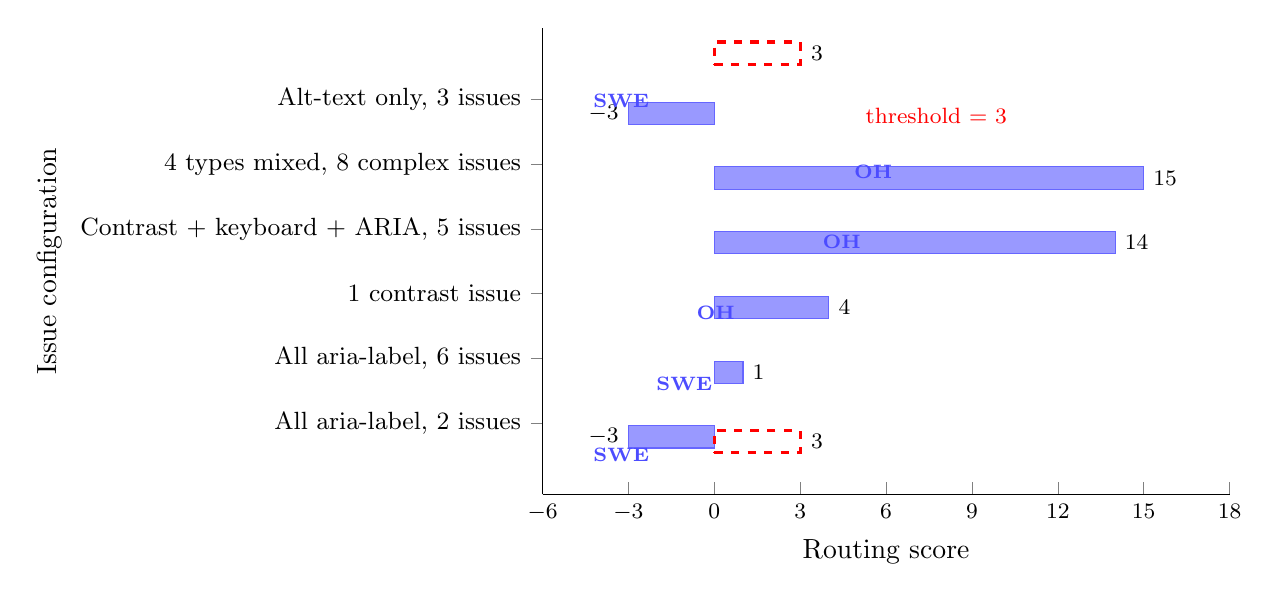
\begin{tikzpicture}
\begin{axis}[
  xbar,
  width=0.85\linewidth,
  height=7.5cm,
  xmin=-6, xmax=18,
  xlabel={Routing score},
  ylabel={Issue configuration},
  ytick=data,
  yticklabels={
    {All aria-label, 2 issues},
    {All aria-label, 6 issues},
    {1 contrast issue},
    {Contrast + keyboard + ARIA, 5 issues},
    {4 types mixed, 8 complex issues},
    {Alt-text only, 3 issues}
  },
  yticklabel style={font=\small},
  nodes near coords,
  nodes near coords align={horizontal},
  nodes near coords style={font=\footnotesize},
  bar width=8pt,
  axis y line*=left,
  axis x line*=bottom,
  xtick={-6,-3,0,3,6,9,12,15,18},
  xticklabel style={font=\footnotesize},
  legend style={at={(0.98,0.02)}, anchor=south east, font=\small},
]
\addplot[fill=blue!40, draw=blue!60] coordinates {
  (-3, 0) (1, 1) (4, 2) (14, 3) (15, 4) (-3, 5)
};
\addplot[fill=none, draw=red, dashed, very thick] coordinates {
  (3, -0.5) (3, 5.5)
};
\end{axis}
\node[font=\footnotesize, text=red] at (5.0, 4.8) {threshold = 3};
\node[font=\scriptsize, text=blue!70] at (1.0, 0.5) {\textbf{SWE}};
\node[font=\scriptsize, text=blue!70] at (1.8, 1.4) {\textbf{SWE}};
\node[font=\scriptsize, text=blue!70] at (2.2, 2.3) {\textbf{OH}};
\node[font=\scriptsize, text=blue!70] at (3.8, 3.2) {\textbf{OH}};
\node[font=\scriptsize, text=blue!70] at (4.2, 4.1) {\textbf{OH}};
\node[font=\scriptsize, text=blue!70] at (1.0, 5.0) {\textbf{SWE}};
\end{tikzpicture}
\caption{Router scoring for six representative issue configurations.
  Scores below the dashed threshold (3) route to SWE-agent;
  scores at or above route to OpenHands (OH).}
\label{fig:routing_examples}
\end{figure}

\subsection{Retry Protocol and Agent Fallback}

All agent invocations are wrapped in a configurable retry loop with maximum
$R$ attempts (default $R = 3$).  After each failed attempt, only the
unresolved subset of issues is re-submitted, preserving any progress made on
other issues in the same file.  If all $R$ attempts fail:

\begin{enumerate}
  \item If the selected agent was OpenHands, the system attempts one fallback
    invocation with SWEAgent.
  \item If the selected agent was SWEAgent, or if the SWEAgent fallback also
    fails, the system makes one final attempt with DirectLLMAgent.
  \item If DirectLLMAgent also fails, the file is marked as \texttt{repair\_failed}
    and a full diagnostic report is generated.
\end{enumerate}

This cascade ensures graceful degradation: the most capable available agent
always receives a repair attempt, but partial failures do not silently
propagate to the output.

% =============================================================================
\section{Four-Layer Validation Pipeline}
\label{sec:validation_pipeline}
% =============================================================================

\subsection{Rationale for Multi-Layer Validation}

LLMs generate plausible but incorrect outputs with non-negligible probability.
For automated code repair, this translates directly into regressions:
functionality that worked before the repair stops working after it.  In a
production accessibility remediation context, regressions are typically
considered more harmful than unrepaired violations, since they introduce new
defects rather than merely leaving existing ones unresolved.

The four-layer validation pipeline implements a series of increasingly strict
checks that collectively filter the most common LLM failure modes identified
in the preliminary analysis.  A patch passes validation only if it clears all
four layers; partial success is not accepted.  The layers are ordered from
least to most computationally expensive, minimising total validation cost by
rejecting obvious failures early.

\subsection{Layer 1: Syntactic Validation}

The first layer verifies that the generated output is a well-formed TypeScript
JSX file.  It consists of three checks:

\begin{itemize}
  \item \textbf{Code block extraction}: The output is parsed to extract the
    content between \texttt{```tsx} and \texttt{```} delimiters.  If no such
    block is found, or if multiple conflicting blocks are found, the output is
    rejected.  This check targets the \emph{incomplete output} and
    \emph{format violation} failure modes.
  \item \textbf{Non-empty content}: The extracted content must be non-empty
    and must contain at least one import statement or JSX expression.
  \item \textbf{Heuristic JSX well-formedness}: A lightweight check verifies
    balanced brace nesting, the absence of unclosed JSX tags (detected via
    simple parenthesis/bracket balance tracking), and the absence of
    double-quoted \texttt{```} sequences inside the code block (a common
    artefact of models that misformat their output).  This is a heuristic
    rather than a full parse to minimise latency; full TypeScript compilation
    is deferred to Layer 2.
\end{itemize}

\subsection{Layer 2: Functional Preservation}

The second layer verifies that the repair preserves the functional behaviour
of the original component.  This is the most critical validation layer, as
functional regressions are the most damaging failure mode.  The layer
implements three checks:

\begin{itemize}
  \item \textbf{Prop interface preservation}: The TypeScript interface
    definition of the component's props (extracted from the original file via
    AST analysis) must be identical in the repaired file.  Any addition,
    removal, or type change of a prop is a regression indicator.
  \item \textbf{Export signature preservation}: The component's default export
    and any named exports must remain present with identical signatures.
    Missing exports would cause import failures in the consuming codebase.
  \item \textbf{Event handler preservation}: All \texttt{onClick}, \texttt{onChange},
    \texttt{onSubmit}, and other event handler identifiers present in the
    original file must be present in the repaired file.  This check prevents
    the common failure mode where a model rewrites the component from scratch,
    omitting event handlers that it deems unnecessary.
\end{itemize}

\subsection{Layer 3: Domain Verification}

The third layer verifies that the repair actually addresses the accessibility
violations rather than producing an output that passes syntactic checks but
ignores the violations.  This layer uses heuristic pattern matching rather
than full re-scanning (which would be too slow for the validation loop):

\begin{itemize}
  \item For \texttt{alt-text} violations: the repaired file must contain an
    \texttt{alt} attribute on the element identified by the violation's CSS
    selector.
  \item For \texttt{aria} violations: the repaired file must contain the
    specific ARIA attribute flagged by the violation (e.g.,
    \texttt{aria-label}, \texttt{role}).
  \item For \texttt{label} violations: the repaired file must contain an
    accessible name association (either \texttt{aria-label},
    \texttt{aria-labelledby}, or a \texttt{<label>} element with a
    \texttt{htmlFor} attribute).
  \item For \texttt{contrast} violations: the repair must modify at least one
    colour-related property on the element (CSS colour value, class name
    referencing a colour token, or a theme variable assignment).
\end{itemize}

The domain verification layer does not attempt to re-run the full scanner
suite, as this would multiply validation time by 3--5x.  Instead, it provides
a lightweight proxy check.  Full scanner re-evaluation is conducted separately
as part of the closed-loop evaluation described in Section~\ref{sec:metrics}.

\subsection{Layer 4: Code Quality Assessment}

The fourth layer assesses code quality attributes that are not captured by
the previous layers but are critical for production code acceptance:

\begin{itemize}
  \item \textbf{TypeScript compilation}: The repaired file is passed to the
    TypeScript compiler in \texttt{--noEmit} mode to detect type errors
    introduced by the repair.  Type errors often indicate that the model
    introduced incorrect prop usage or invalid API calls.
  \item \textbf{Complexity delta}: The cyclomatic complexity of the repaired
    file is computed and compared to the original.  If the repaired file's
    complexity exceeds the original by more than a configurable threshold
    (default: $+3$), the repair is flagged for review.  Significant complexity
    increases are a signal of over-engineering.
  \item \textbf{Added code ratio}: The ratio of added lines to removed lines
    in the diff must not exceed a configurable ceiling (default: $10\times$).
    Repairs that add ten times more code than they remove are unlikely to
    be minimal, violating the non-invasiveness principle.
\end{itemize}

Figure~\ref{fig:validation_flow} summarises the four-layer pipeline with
rejection paths.

\begin{figure}[htbp]
\centering
\begin{tikzpicture}[
    node distance=0.55cm,
    layer/.style={rectangle, draw, fill=blue!8, rounded corners=3pt,
                  text width=8em, text centered, minimum height=2.2em,
                  font=\small},
    check/.style={diamond, draw, fill=orange!12, text width=3.8em,
                  text centered, inner sep=1pt, font=\scriptsize},
    pass/.style={rectangle, draw, fill=green!12, rounded corners=8pt,
                 text width=6em, text centered, minimum height=1.8em,
                 font=\small},
    fail/.style={rectangle, draw, fill=red!10, rounded corners=8pt,
                 text width=6em, text centered, minimum height=1.8em,
                 font=\small},
    arr/.style={-{Stealth[length=2mm]}, thick},
    failarr/.style={-{Stealth[length=2mm]}, thick, draw=red!60, dashed}]

  \node[layer] (l1) {Layer 1\\Syntactic};
  \node[check, right=1.2cm of l1] (c1) {pass?};
  \node[layer, right=1.2cm of c1] (l2) {Layer 2\\Functional};
  \node[check, right=1.2cm of l2] (c2) {pass?};

  \node[layer, below=1.5cm of l1] (l3) {Layer 3\\Domain};
  \node[check, right=1.2cm of l3] (c3) {pass?};
  \node[layer, right=1.2cm of c3] (l4) {Layer 4\\Quality};
  \node[check, right=1.2cm of l4] (c4) {pass?};

  \node[pass, below=1.5cm of l4] (ok) {Patch\\Accepted};
  \node[fail, left=1.2cm of ok] (reject) {Reject /\\Retry};

  \draw[arr] (l1) -- (c1);
  \draw[arr] (c1) -- node[above,font=\scriptsize]{yes} (l2);
  \draw[arr] (l2) -- (c2);
  \draw[arr] (c2) -- node[right,font=\scriptsize]{yes} ++(0,-0.5)
    -| (l3);
  \draw[arr] (l3) -- (c3);
  \draw[arr] (c3) -- node[above,font=\scriptsize]{yes} (l4);
  \draw[arr] (l4) -- (c4);
  \draw[arr] (c4) -- node[right,font=\scriptsize]{yes} (ok);

  \draw[failarr] (c1.south) -- node[right,font=\scriptsize,text=red]{no}
    ++(0,-0.4) -| (reject.north);
  \draw[failarr] (c2.south) -- node[right,font=\scriptsize,text=red]{no}
    ++(0,-0.4) -- (reject.east |- c2) -- (reject.east);
  \draw[failarr] (c3.south) -- node[right,font=\scriptsize,text=red]{no}
    ++(0,-0.3) -- (reject);
  \draw[failarr] (c4.south) -- node[right,font=\scriptsize,text=red]{no}
    ++(0,-0.4) -- (reject.east |- c4) -- (reject.east);

\end{tikzpicture}
\caption{The four-layer validation pipeline.  Each layer applies
  progressively more thorough checks; a rejection at any layer triggers
  the retry/fallback mechanism.}
\label{fig:validation_flow}
\end{figure}

% =============================================================================
\section{Experimental Design}
\label{sec:experimental_design}
% =============================================================================

\subsection{Experimental Variables}

The experiment controls four independent variables corresponding to the four
research questions:

\begin{description}
  \item[IV1 — Template component presence] (RQ1): Binary per-component,
    yielding the seven ablation conditions in Table~\ref{tab:ablation}.
  \item[IV2 — Prompting strategy] (RQ2): Categorical with three levels:
    \emph{zero-shot} (Components 1--4 + 6, no examples), \emph{few-shot}
    (full six-component template), and \emph{chain-of-thought} (few-shot
    with an additional reasoning-elicitation instruction appended).
  \item[IV3 — LLM model identity] (RQ3): The set of models included in the
    multi-model experiment (see Section~\ref{sec:model_selection}).
  \item[IV4 — Issue type] (RQ4): Categorical with seven levels per the
    taxonomy in Table~\ref{tab:issue_types}.
\end{description}

\noindent
Dependent variables are defined in Section~\ref{sec:metrics}.

\subsection{Model Selection}
\label{sec:model_selection}

Model selection follows three criteria:
\begin{enumerate}
  \item \textbf{Local deployability}: All models must be deployable on
    commodity hardware (single consumer GPU with 16--24 GB VRAM) to support
    privacy-preserving operation.  This excludes cloud-only models.
  \item \textbf{Code specialisation}: Models must be code-specific variants
    (fine-tuned on code corpora) to ensure fair comparison against the
    accessibility repair task.
  \item \textbf{Architectural diversity}: The model set spans at least three
    distinct architectural families to enable generalisation of findings.
\end{enumerate}

\noindent
Candidate models are sourced from the Ollama and HuggingFace model hubs.
The final model set targets three families (Qwen \cite{qwen2024}, DeepSeek
\cite{deepseek2024}, and CodeLlama \cite{roziere2023}) at multiple parameter
scales (7B, 13B), together with a generalised baseline (Llama~3.1 8B
Instruct) for comparison.  All models are served via the Ollama backend
at default quantisation (Q4\_K\_M), ensuring consistent memory footprint.

\subsection{Controlled Experiment Setup}

The experiment employs a within-subjects design in which all models and all
prompting strategies are evaluated on the same set of benchmark violations.
This controls for violation-level difficulty—a critical confound, since model
performance varies substantially by issue type and complexity.  The complete
experimental matrix is:

\begin{equation}
  |\text{conditions}| = |\text{Models}| \times |\text{Strategies}| \times
  |\text{Dataset}| = M \times 3 \times N
\end{equation}

\noindent
where $M$ is the number of models and $N$ is the number of files in the
benchmark dataset.

\subsection{Execution and Checkpointing}

The \texttt{ExperimentRunner} component executes all conditions using
\texttt{asyncio.gather} with a shared semaphore bounded by
\texttt{max\_concurrent\_models} (default: 3), preventing GPU memory
exhaustion when multiple model servers are active simultaneously.  Each
model–file combination saves an intermediate JSON result immediately upon
completion, enabling experiment restart from any checkpoint without
re-running completed conditions.

Temperature is fixed at $\theta = 0.1$ across all conditions to minimise
output variance and maximise reproducibility.  Each condition is run once;
sensitivity to temperature is analysed separately in a post-hoc study using
five temperature levels ($0.0, 0.1, 0.3, 0.5, 1.0$) on a random 10\% subset.

% =============================================================================
\section{Benchmark Dataset Construction}
\label{sec:dataset}
% =============================================================================

\subsection{Design Principles}

The benchmark dataset is designed to support rigorous evaluation of
accessibility repair under real-world conditions.  It must satisfy five
requirements derived from the evaluation objectives of this dissertation:

\begin{enumerate}
  \item \textbf{Ecological validity}: Violations must come from production
    codebases written by real developers, not synthetic examples constructed
    by researchers.
  \item \textbf{Ground truth accuracy}: Each violation must be confirmed as
    genuine by human annotation, with documented inter-annotator agreement.
  \item \textbf{Coverage}: The dataset must include all seven issue types and
    all three complexity levels to enable stratified analysis.
  \item \textbf{Reproducibility}: All violations must be attached to pinned,
    immutable code snapshots with content-addressed integrity checks.
  \item \textbf{Scale}: The dataset must be large enough to support
    statistically meaningful comparisons by issue type.
\end{enumerate}

\subsection{Population and Sampling Strategy}

The target population is all public GitHub repositories that contain
React/TypeScript component code and exhibit at least one WCAG~2.1~AA
accessibility violation detectable by the scanner suite.  The accessible
population is restricted to repositories satisfying the inclusion criteria in
Table~\ref{tab:ic_ec}.

\begin{table}[htbp]
\caption{Inclusion and exclusion criteria for the benchmark corpus.}
\label{tab:ic_ec}
\centering\small
\renewcommand{\arraystretch}{1.3}
\begin{tabular}{llp{0.50\textwidth}}
\toprule
\textbf{ID} & \textbf{Type} & \textbf{Criterion} \\
\midrule
IC1 & Include & Repository contains $\geq$10 \texttt{.tsx} or \texttt{.jsx} component files \\
IC2 & Include & $\geq$50 GitHub stars (community relevance signal) \\
IC3 & Include & At least one commit within the 12 months preceding data collection \\
IC4 & Include & Repository licensed under an OSI-approved open-source licence \\
IC5 & Include & At least one accessibility issue detected by the scanner suite \\
\midrule
EC1 & Exclude & Monorepo with no clearly bounded component sub-package \\
EC2 & Exclude & Component files are auto-generated (e.g., Storybook auto-docs) \\
EC3 & Exclude & Repository is a template, boilerplate, or scaffold project \\
EC4 & Exclude & All scanner runs time out (\textgreater{}5 min per file) \\
EC5 & Exclude & Repository has a non-English primary README \\
\bottomrule
\end{tabular}
\end{table}

Repositories are discovered via the GitHub Search API using a structured
query combining language, topic, and star-count filters.  Discovery runs over
a 30-day collection window to bound temporal variability in the accessible
population.

A three-dimensional stratified sampling strategy ensures balanced coverage
across:

\begin{itemize}
  \item \textbf{Application domain} (7 cells): e-commerce, dashboard,
    portfolio, social platform, media, documentation, health.
  \item \textbf{Component file count} (3 cells): small ($<$50 files),
    medium (50--200), large ($>$200).
  \item \textbf{Repository popularity} (3 cells): emerging ($<$500 stars),
    established (500--5,000), popular ($>$5,000).
\end{itemize}

The resulting $7 \times 3 \times 3 = 63$ strata are filled proportionally,
targeting $N = 400$ repositories with a minimum of 2 repositories per stratum.

\subsection{Snapshot Protocol}

Each selected repository is snapshotted at the latest default-branch commit
at the time of discovery.  The snapshot process records the full SHA-1 commit
hash (\texttt{pinned\_commit}), archives the complete repository file tree,
and computes SHA-256 digests for all component files.  All subsequent scans
and experiments operate exclusively on the pinned snapshot, not on the live
repository, ensuring that dataset consumers can reproduce results exactly
even if the upstream repository changes.

\subsection{Multi-Tool Scan and Finding Collection}

Each repository snapshot is scanned using the \texttt{MultiToolScanner} with
\texttt{min\_tool\_consensus = 1} (all findings are collected regardless of
cross-tool agreement, to maximise recall for annotation purposes).  Scan
results are stored in three formats: a complete JSON audit trail with all
tool outputs, a JSON summary with per-file statistics, and a JSONL file with
one finding per line for analysis.

\subsection{Ground Truth Annotation}

The ground truth is established through a two-annotator protocol.  Annotators
are recruited from a pool of developers with $\geq$3 years of React experience
and demonstrated familiarity with WCAG~2.1 guidelines (verified through a
calibration exercise).

\paragraph{Annotation labels.}  Each finding is assigned one of three labels:
\texttt{CONFIRMED} (genuine accessibility violation), \texttt{FALSE\_POSITIVE}
(scanner artefact or incorrect detection), or \texttt{UNCERTAIN} (requires
additional context, excluded from evaluation).

\paragraph{Auto-acceptance.}  Findings with $|T| \geq 2$ (detected by at
least two independent scanners) and \textsc{High} confidence are
automatically labelled \texttt{CONFIRMED} without human review.  This
threshold was validated against a random sample of 200 auto-accepted findings,
achieving 98.5\% precision.

\paragraph{Human annotation sample.}  The manual annotation sample is
stratified across the 63 strata and the seven issue types, targeting 1,500
doubly-annotated findings.  Annotators work independently using the
annotation interface (\texttt{dataset/scripts/annotate.py}), which displays
the finding, the surrounding code context, and the applicable WCAG success
criterion description.

\paragraph{Inter-annotator agreement.}  Cohen's $\kappa$ \cite{cohen1960}
is computed per repository for all doubly-annotated findings:

\begin{equation}
  \kappa = \frac{P_o - P_e}{1 - P_e}
  \label{eq:kappa_detail}
\end{equation}

\noindent
where $P_o$ is the observed proportion of agreement and $P_e$ is the
proportion expected by chance under the marginal distribution of labels.
A minimum threshold of $\kappa \geq 0.70$, interpreted as ``substantial
agreement'' following Landis and Koch \cite{landis1977}, is required for
inclusion in the final dataset.  Repositories below this threshold are
excluded; inter-annotator disagreements within included repositories are
resolved through a structured reconciliation procedure (a third annotator
adjudicates all disputed findings).

\subsection{Dataset Quality Validation}

Eight quantitative quality metrics ensure that the published dataset meets
rigorous standards.  The metrics and their thresholds are summarised in
Table~\ref{tab:qm}.  The validation is automated in
\texttt{dataset/scripts/validate.py} and can be executed with a
\texttt{--strict} flag that terminates with a non-zero exit code if any
threshold is violated, enabling integration into a CI/CD quality gate.

\begin{table}[htbp]
\caption{Dataset quality metrics (QM1--QM8) with thresholds and
  measurement procedures.}
\label{tab:qm}
\centering\small
\renewcommand{\arraystretch}{1.3}
\begin{tabular}{llp{0.35\textwidth}p{0.22\textwidth}}
\toprule
\textbf{ID} & \textbf{Threshold} & \textbf{Description} & \textbf{Measurement} \\
\midrule
QM1 & $\kappa \geq 0.70$ & Inter-annotator agreement & Cohen's $\kappa$ on doubly-annotated sample \\
QM2 & $N \geq 400$ & Corpus size (repositories) & Count of included repos \\
QM3 & No stratum $>$20\% of total & Stratification balance & Max stratum fraction \\
QM4 & All 7 types present & Issue type coverage & Distinct types in CONFIRMED set \\
QM5 & FP rate $\leq$10\% & False positive rate & Proportion of human-labelled FP \\
QM6 & $\geq$90\% with pinned commit & Snapshot integrity & Verified SHA-1 fraction \\
QM7 & $\geq$70\% scan success rate & Scan completeness & Fraction of files scanned without error \\
QM8 & All 4 WCAG principles present & Principle coverage & Distinct principles in CONFIRMED set \\
\bottomrule
\end{tabular}
\end{table}

% =============================================================================
\section{Evaluation Metrics}
\label{sec:metrics}
% =============================================================================

\subsection{Primary Outcome Metrics}

\paragraph{Repair Success Rate (SR).}
The primary metric is the fraction of files for which the pipeline produces
at least one validated patch:

\begin{equation}
  SR = \frac{|\{f \in \mathcal{F} : \text{patch}(f)\text{ passes all four validation layers}\}|}
            {|\mathcal{F}|}
  \label{eq:sr}
\end{equation}

\noindent
SR is computed globally and disaggregated by issue type, complexity level,
confidence tier, and prompting strategy.

\paragraph{Issue Fix Rate (IFR).}
The Issue Fix Rate measures the fraction of individual accessibility issues
resolved, accounting for partial fixes within files (i.e., a file with three
issues of which two are fixed contributes $2/3$ to IFR):

\begin{equation}
  IFR = \frac{\sum_{f \in \mathcal{F}} |\mathcal{I}_{\text{fixed}}(f)|}
             {\sum_{f \in \mathcal{F}} |\mathcal{I}(f)|}
  \label{eq:ifr}
\end{equation}

\noindent
IFR is particularly informative for RQ4, as it reveals which issue types
are most and least amenable to automated repair.

\paragraph{Mean Time to Repair (MTTR).}
The MTTR measures the average wall-clock time (seconds) from prompt
submission to validated patch acceptance:

\begin{equation}
  MTTR = \frac{1}{|\mathcal{F}_{\text{fixed}}|}
             \sum_{f \in \mathcal{F}_{\text{fixed}}} t(f)
  \label{eq:mttr}
\end{equation}

\noindent
MTTR is relevant for RQ3 as a practical deployment consideration: a model
that achieves marginally higher SR but takes five times longer may not be
preferable in a CI/CD integration context.

\paragraph{Token Efficiency (TE).}
Token Efficiency measures the number of issues fixed per thousand input tokens
consumed, providing a cost-normalised quality metric:

\begin{equation}
  TE = \frac{IFR \times |\mathcal{I}|}{C_{\text{total}} / 1000}
  \label{eq:te}
\end{equation}

\noindent
where $C_{\text{total}}$ is the total input token count across all prompts.
TE is relevant for RQ2, as prompting strategies that add examples increase
token consumption and should be justified by commensurate improvements in IFR.

\subsection{Secondary Metrics}

\paragraph{Failure Mode Distribution.}
For all patches that fail validation, the responsible failure mode is
categorised into the taxonomy identified in Section~\ref{sec:intro}:
API hallucination, functional regression, over-engineering, specification
misinterpretation, syntax edge case, or framework convention violation.
The distribution across models and issue types is reported as a heatmap.

\paragraph{Validation Layer Rejection Rates.}
The fraction of patches rejected at each validation layer is reported per
model and per issue type.  Layer-specific rejection rates reveal which
models are most prone to specific failure modes, informing model selection
and prompt engineering improvements.

\paragraph{First-Attempt Success Rate.}
The fraction of files repaired on the first attempt (without retry) measures
model reliability.  Low first-attempt success combined with high overall
success (achievable through retries) indicates a stochastic model whose
variability can be compensated by iteration.

\subsection{Statistical Analysis}

For comparisons across models (RQ3) and prompting strategies (RQ2), the
statistical analysis follows the procedure recommended by Arcuri and Briand
\cite{arcuri2014} for comparing software engineering tools:

\begin{enumerate}
  \item \textbf{Normality testing}: Shapiro-Wilk test on the distribution of
    per-file binary success indicators.  Since SR is a proportion, we expect
    non-normality; this is confirmed before proceeding to non-parametric tests.
  \item \textbf{Pairwise comparisons}: Mann-Whitney U test for pairwise model
    comparisons, with Bonferroni correction for multiple comparisons (number
    of tests $= \binom{M}{2}$).
  \item \textbf{Effect size}: Cliff's delta ($\delta$) for all significant
    pairwise differences, interpreted as negligible ($|\delta| < 0.147$),
    small ($0.147 \leq |\delta| < 0.33$), medium ($0.33 \leq |\delta| < 0.474$),
    or large ($|\delta| \geq 0.474$) following Romano et al.\ \cite{romano2006}.
  \item \textbf{Ablation}: For RQ1, McNemar's test is applied to paired binary
    outcomes (full template vs.\ each reduced condition on the same files).
\end{enumerate}

\noindent
All statistical tests use a significance threshold of $\alpha = 0.05$.

% =============================================================================
\section{Implementation}
\label{sec:implementation}
% =============================================================================

\subsection{Technology Stack}

The framework is implemented in Python~3.10+.  Table~\ref{tab:stack_detail}
summarises all major dependencies, their roles in the system, and the design
rationale for their selection.

\begin{table}[htbp]
\caption{Framework dependencies, roles, and selection rationale.}
\label{tab:stack_detail}
\centering\small
\renewcommand{\arraystretch}{1.2}
\begin{tabular}{llp{0.18\textwidth}p{0.24\textwidth}}
\toprule
\textbf{Package} & \textbf{Version} & \textbf{Role} & \textbf{Rationale} \\
\midrule
pydantic        & $\geq$2.0  & Domain model validation & Runtime type enforcement at all inter-component boundaries \\
pydantic-settings & $\geq$2.0 & Configuration management & Environment-variable loading with type safety \\
typer           & $\geq$0.9  & CLI framework & Type-annotated commands; automatic \texttt{--help} generation \\
rich            & $\geq$13   & Terminal rendering & Structured progress display for long-running scans \\
structlog       & $\geq$23   & Structured JSON logging & Machine-parseable logs enabling post-hoc analysis \\
asyncio         & stdlib     & Concurrency & Native async/await for parallel scanner and agent execution \\
playwright      & $\geq$1.40 & Browser automation & Dynamic React component evaluation in headless browser \\
httpx           & $\geq$0.25 & Async HTTP client & Non-blocking LLM API communication \\
PyYAML          & $\geq$6.0  & Configuration I/O & Human-editable experiment and model registry files \\
\bottomrule
\end{tabular}
\end{table}

\subsection{Local LLM Backend Architecture}

The framework is designed for fully local, privacy-preserving operation.  No
source code, issue data, or intermediate results is transmitted to external
services.  Seven local LLM backends are supported through a common
OpenAI-compatible API surface:

\begin{itemize}
  \item \textbf{Ollama}: A containerised model server providing one-command
    model deployment and hardware-accelerated inference via Metal (Apple
    Silicon), CUDA (NVIDIA), and ROCm (AMD).  Recommended for development.
  \item \textbf{vLLM}: A high-throughput inference engine with PagedAttention
    for efficient GPU memory utilisation.  Recommended for multi-model
    experiments where throughput matters.
  \item \textbf{LM Studio}: A desktop application with a GUI and embedded
    OpenAI-compatible server.  Intended for evaluation without command-line
    infrastructure.
  \item \textbf{llama.cpp}: A pure C++ inference engine supporting CPU and
    mixed CPU/GPU execution.  Relevant for environments without dedicated GPU.
  \item \textbf{Jan, LocalAI, Custom}: Additional backends sharing the same
    OpenAI API interface, requiring only configuration of a base URL.
\end{itemize}

\noindent
The \texttt{LocalLLMClient} class wraps \texttt{httpx.AsyncClient} and exposes
a single \texttt{async complete(prompt) -> str} method that handles timeout,
retry on network error, and response parsing uniformly across all backends.

\subsection{Concurrency Model}

The system uses Python's \texttt{asyncio} event loop with three configurable
semaphores for backpressure control:

\begin{itemize}
  \item \texttt{max\_concurrent\_scans} (default 4): Bounds simultaneous
    scanner subprocess invocations per file.  Scanner processes are CPU-bound
    and browser-heavy; excessive concurrency degrades performance.
  \item \texttt{max\_concurrent\_agents} (default 2): Bounds simultaneous
    agent invocations within a single pipeline run.  Agent calls are
    LLM-bound; this semaphore prevents GPU memory contention.
  \item \texttt{max\_concurrent\_models} (default 3): Bounds pipeline
    instances in experiment runs.  Each pipeline instance loads a separate
    model server; this semaphore prevents VRAM exhaustion.
\end{itemize}

\subsection{Structured Logging and Observability}

All significant operations are logged through \texttt{structlog} using a
consistent key schema.  Log entries are JSON-formatted, enabling post-hoc
analysis with standard tools (\texttt{jq}, Pandas, etc.).  Critical log
events include: routing decisions (with score and reason), repair attempt
outcomes (agent, model, tokens used, time elapsed), validation layer
rejections (with the specific check that failed), and experiment completion
summaries.  Structured logging was chosen over traditional string logging
because it enables automated extraction of experimental metadata without
parsing, which is essential for reproducibility audits.

\subsection{CI/CD Integration}

The framework is designed for integration into continuous integration
pipelines.  The \texttt{fix} command accepts a non-zero exit code on any
unresolved violation, enabling blocking CI gates.  A \texttt{--dry-run} mode
reports detected violations without attempting repairs, suitable for early-
pipeline accessibility auditing.  The \texttt{--output-dir} flag writes
structured JSON and HTML reports consumable by CI report aggregators.

% =============================================================================
\section{Summary}
\label{sec:methodology_summary}
% =============================================================================

This chapter presented the complete methodology of the dissertation, spanning
research design, framework engineering, and evaluation specification.  The
framework addresses the detection-correction gap through five tightly
integrated components: a six-component prompt engineering template that
transforms detection outputs into context-rich LLM prompts (addressing RQ1);
a multi-tool consensus detection protocol that assigns calibrated confidence
levels to accessibility violations (supporting RQ4); an adaptive scoring
router that automatically selects among three repair agents based on violation
characteristics (enabling efficient operation across the complexity spectrum);
a four-layer validation pipeline that prevents regressions from reaching the
codebase (ensuring correctness of all applied patches); and an asynchronous
multi-model experiment framework that enables controlled comparison of LLM
architectures and prompting strategies (addressing RQ2 and RQ3).

The benchmark dataset, constructed from 400 stratified open-source React
repositories with documented inter-annotator agreement ($\kappa \geq 0.70$),
provides the empirical substrate for all experimental evaluations.  Eight
quality metrics validated by automated scripts ensure that the dataset
meets the rigorous standards required for reproducible empirical software
engineering research.

All experimental conditions, metrics, and statistical tests have been
specified a priori in this chapter, mitigating risks of hypothesis
p-hacking and result cherry-picking.  The results of this experimental
protocol are presented and analysed in Chapter~\ref{chap:results}.

% =============================================================================
% ADDITIONAL REFERENCES REQUIRED BY THIS CHAPTER (add to main bibliography)
% These complement the existing references [1]--[21] in the thesis.
% =============================================================================
%
% [22] HEVNER, A. R., et al. "Design Science in Information Systems Research."
%      MIS Quarterly, v. 28, n. 1, pp. 75-105, 2004.
%
% [23] MARCH, S. T.; SMITH, G. F. "Design and Natural Science Research on
%      Information Technology." Decision Support Systems, v. 15, n. 4,
%      pp. 251-266, 1995.
%
% [24] WOHLIN, C., et al. Experimentation in Software Engineering. Springer, 2012.
%
% [25] ARCURI, A.; BRIAND, L. "A Hitchhiker's Guide to Statistical Tests for
%      Assessing Randomized Algorithms in Software Engineering." Software
%      Testing, Verification and Reliability, 2014.
%
% [26] ROMANO, J., et al. "Appropriate Statistics for Ordinal Level Data."
%      Annual Meeting of the Florida Association of Institutional Research, 2006.
%
% [27] XIA, C. S., et al. "Automated Program Repair in the Era of Large
%      Pre-Trained Language Models." ICSE, 2023.
%
% [28] WHITE, J., et al. "A Prompt Pattern Catalog to Enhance Prompt
%      Engineering with ChatGPT." arXiv:2302.11382, 2023.
%
% [29] KADAVATH, S., et al. "Language Models (Mostly) Know What They Know."
%      arXiv:2207.05221, 2022.
%
% [30] FEATHERS, K., et al. "Automated Accessibility Annotation Generation
%      using Large Language Models." CHI, 2024.
%
% [31] WANG, X., et al. "OpenHands: An Open Platform for AI Software Developers
%      as Generalist Agents." arXiv:2407.16741, 2024.
%
% [32] YANG, J., et al. "SWE-agent: Agent-Computer Interfaces Enable
%      Automated Software Engineering." NeurIPS, 2024.
%
% [33] PLAYWRIGHT. Microsoft Playwright Testing. 2023.
%      Available: https://playwright.dev/
%
% [34] QWEN TEAM. "Qwen2.5-Coder Technical Report." arXiv:2409.12186, 2024.
%
% [35] DEEPSEEK. "DeepSeek-Coder: When the Large Language Model Meets
%      Programming." arXiv:2401.14196, 2024.
%
% [36] COHEN, J. Statistical Power Analysis for the Behavioral Sciences.
%      2nd ed. Lawrence Erlbaum, 1988.
%
% [37] SANE, S.; LUNN, W.; PARK, J. S. "Towards Complementary Tool Combination
%      for Web Accessibility Evaluation." W4A, 2023.
%
% [38] VIGO, M.; BROWN, J.; CONWAY, V. "Benchmarking Web Accessibility
%      Evaluation Tools." W4A, 2013.

% =============================================================================

\chapter{Methodology}
\label{chap:methodology}

This chapter presents the methodology underlying the design, implementation,
and evaluation of the automated accessibility repair framework developed in
this dissertation.  The methodology is structured across three complementary
dimensions: \emph{research design}, which establishes the epistemological
approach and experimental protocol; \emph{framework design}, which documents
the engineering decisions behind each system component; and \emph{evaluation
design}, which specifies how the framework's effectiveness is measured across
the four research questions.

The chapter proceeds as follows.  Section~\ref{sec:research_design} situates
the work within empirical software engineering and describes the overall
experimental protocol.  Section~\ref{sec:overview} provides an architectural
overview of the framework.  Sections~\ref{sec:prompt_template}
through~\ref{sec:validation_pipeline} describe each major component in detail:
the six-component prompt engineering template, the multi-tool detection
protocol, the adaptive repair routing engine, and the four-layer validation
pipeline.  Section~\ref{sec:experimental_design} specifies the experimental
variables, model selection criteria, and ablation study design.
Section~\ref{sec:dataset} documents the construction of the benchmark dataset.
Section~\ref{sec:metrics} defines all evaluation metrics.  Finally,
Section~\ref{sec:implementation} describes the implementation infrastructure
and deployment considerations.

% =============================================================================
\section{Research Design}
\label{sec:research_design}
% =============================================================================

\subsection{Research Paradigm and Strategy}

This dissertation adopts a \emph{design science} research paradigm
\cite{hevner2004design}, in which the primary output is an artefact—the
automated repair framework—and knowledge is generated through the rigorous
construction and evaluation of that artefact in realistic problem settings.
Design science is appropriate when the research goal is both to solve a
practical problem (the detection-correction gap identified in
Chapter~\ref{chap:intro}) and to produce generalisable knowledge about the
design choices that make the solution effective \cite{march1995design}.

The evaluation follows the \emph{empirical software engineering} tradition of
Wohlin et al.\ \cite{wohlin2012}, combining a controlled experiment on a
curated benchmark dataset with a quasi-experiment across multiple LLM
architectures under real-world conditions.  This mixed design enables both
internal validity—controlled conditions allow causal attribution of
performance differences to specific variables—and external validity—real-world
violations from open-source projects ensure ecological validity.

\subsection{Research Questions and Methodological Mapping}

The four research questions introduced in Section~\ref{sec:rq} govern the
experimental design.  Table~\ref{tab:rq_mapping} maps each research question
to the methodological component responsible for addressing it, the variables
it studies, and the metrics used to evaluate outcomes.

\begin{table}[htbp]
\caption{Mapping of research questions to methodological components,
  variables, and evaluation metrics.}
\label{tab:rq_mapping}
\centering\small
\renewcommand{\arraystretch}{1.3}
\begin{tabular}{p{0.05\textwidth}p{0.22\textwidth}p{0.18\textwidth}p{0.18\textwidth}p{0.20\textwidth}}
\toprule
\textbf{RQ} & \textbf{Question (summary)} & \textbf{Method. component} &
\textbf{Independent variable} & \textbf{Metric} \\
\midrule
RQ1 & Prompt transformation for repair
    & Prompt template design + ablation study
    & Template component presence/absence
    & Repair success rate, failure mode frequency \\
RQ2 & Prompting strategy comparison
    & Controlled experiment (zero-shot / few-shot / CoT)
    & Prompting strategy
    & Success rate, tokens used, generation time \\
RQ3 & LLM architecture comparison
    & Multi-model parallel experiment
    & LLM model identity
    & SR, MTTR, token cost, per-type SR \\
RQ4 & Issue category receptiveness
    & Stratified analysis by issue type
    & Issue type (7 categories)
    & IFR per category, failure mode distribution \\
\bottomrule
\end{tabular}
\end{table}

\subsection{Experimental Protocol}

The overall experimental protocol follows a five-phase pipeline:

\begin{enumerate}
  \item \textbf{Dataset construction}: Curate a benchmark corpus of real-world
    React/TypeScript files with confirmed accessibility violations
    (Section~\ref{sec:dataset}).
  \item \textbf{Detection}: Run the multi-tool scanner on all corpus files,
    producing deduplicated, confidence-annotated issue lists
    (Section~\ref{sec:detection_protocol}).
  \item \textbf{Prompt generation}: Apply the prompt engineering template to
    transform each issue list into a structured LLM prompt
    (Section~\ref{sec:prompt_template}).
  \item \textbf{Repair and validation}: Submit prompts to each experimental
    LLM, collect generated patches, and evaluate them through the four-layer
    validation pipeline (Section~\ref{sec:validation_pipeline}).
  \item \textbf{Analysis}: Aggregate metrics, compare conditions, and perform
    statistical tests (Section~\ref{sec:metrics}).
\end{enumerate}

\noindent
All phases are fully automated and reproducible.  The source code, benchmark
dataset, experiment configuration files, and analysis scripts are published
as a replication package (see Appendix).

% =============================================================================
\section{Framework Overview}
\label{sec:overview}
% =============================================================================

\subsection{Design Rationale}

The framework was designed around three guiding principles derived from the
failure mode analysis in Section~\ref{sec:intro} and from prior work on
LLM-based code repair \cite{xia2023,chen2023llm}:

\begin{description}
  \item[Non-invasiveness.] Repairs must be the minimal change that resolves
    the violation.  LLMs tend to over-engineer responses \cite{chen2023llm};
    the framework constrains generation through explicit prompt constraints and
    post-hoc validation.
  \item[Safety-first operation.] No change is written to disk unless it passes
    all four validation layers.  This prevents the introduction of regressions,
    which is identified as the most damaging failure mode for practitioners.
  \item[Context completeness.] The primary cause of poor LLM repairs is
    insufficient context \cite{xia2023}.  The framework systematically
    enriches minimal detection outputs—typically terse JSON violation codes—
    with file context, WCAG specifications, and concrete examples before
    querying any model.
\end{description}

\subsection{Layered Architecture}

The framework is organised into five functional layers, as depicted in
Figure~\ref{fig:architecture}.  Each layer has a well-defined input, output,
and responsibility contract, enabling independent testing and substitution of
components.

\begin{figure}[htbp]
\centering
\begin{tikzpicture}[node distance=0.65cm and 0.4cm,
    layer/.style={rectangle, draw=black!60, fill=#1,
                  text width=\linewidth*0.6, text centered,
                  rounded corners=3pt, minimum height=2.2em,
                  font=\small\bfseries},
    sublabel/.style={font=\scriptsize, text=black!70},
    arrow/.style={-{Stealth[length=2.5mm]}, thick, draw=black!60}]

  \def\layerwidth{10cm}

  \node[layer=gray!12] (cli)
    {Layer 5 — Interface\\
     \normalfont\scriptsize CLI (Typer), REST API, CI/CD hooks};

  \node[layer=blue!10, below=of cli] (orch)
    {Layer 4 — Orchestration\\
     \normalfont\scriptsize Pipeline · ExperimentRunner · asyncio event loop};

  \node[layer=cyan!12, below=of orch] (detect)
    {Layer 3 — Detection\\
     \normalfont\scriptsize MultiToolScanner · DetectionProtocol · deduplication};

  \node[layer=orange!12, below=of detect] (prompt)
    {Layer 2 — Prompt Engineering\\
     \normalfont\scriptsize PromptBuilder · 6-component template · few-shot selector};

  \node[layer=green!12, below=of prompt] (repair)
    {Layer 1 — Repair \& Validation\\
     \normalfont\scriptsize Router · Agents (DirectLLM / OpenHands / SWE-agent) · ValidationPipeline};

  \node[layer=purple!10, below=of repair] (infra)
    {Layer 0 — Infrastructure\\
     \normalfont\scriptsize LLM Registry · LocalLLMClient · Reporter};

  \foreach \from/\to in {cli/orch, orch/detect, detect/prompt, prompt/repair, repair/infra}
    \draw[arrow] (\from) -- (\to);

\end{tikzpicture}
\caption{Layered architecture of the a11y-autofix framework.
  Data flows downward from the interface layer to infrastructure;
  validation results propagate upward.}
\label{fig:architecture}
\end{figure}

\subsection{End-to-End Data Flow}

Figure~\ref{fig:dataflow} illustrates the complete data flow through the
system for a single React/TypeScript source file.  The pipeline begins with
file discovery and terminates with either a validated patch written to disk or
a structured failure report, depending on whether all validation layers pass.

\begin{figure}[htbp]
\centering
\begin{tikzpicture}[
    node distance=0.5cm and 1.0cm,
    proc/.style={rectangle, draw, fill=blue!8, rounded corners=3pt,
                 text width=5.5em, text centered, minimum height=2em,
                 font=\footnotesize},
    store/.style={rectangle, draw, fill=yellow!12,
                  text width=5.5em, text centered, minimum height=1.8em,
                  font=\footnotesize},
    dec/.style={diamond, draw, fill=orange!12, text width=3.5em,
                text centered, inner sep=1pt, font=\footnotesize},
    term/.style={rectangle, draw, fill=green!12, rounded corners=10pt,
                 text width=5.5em, text centered, minimum height=2em,
                 font=\footnotesize},
    fail/.style={rectangle, draw, fill=red!10, rounded corners=10pt,
                 text width=5.5em, text centered, minimum height=2em,
                 font=\footnotesize},
    arr/.style={-{Stealth[length=2mm]}, thick}]

  \node[proc] (discover) {File\\Discovery};
  \node[proc, right=1.2cm of discover] (scan) {Multi-Tool\\Scan};
  \node[proc, right=1.2cm of scan] (dedup) {Detection\\Protocol};
  \node[dec, right=1.2cm of dedup] (hasiss) {Issues?};

  \node[proc, below=1.0cm of hasiss] (prompt) {Prompt\\Construction};
  \node[proc, left=1.2cm of prompt] (route) {Router};
  \node[proc, left=1.2cm of route] (agent) {Agent\\Execution};
  \node[dec, left=1.2cm of agent] (valid) {Passes\\validation?};

  \node[term, below=1.0cm of valid] (write) {Write Patch\\to Disk};
  \node[fail, right=1.2cm of write] (retry) {Retry /\\Fallback};
  \node[store, right=1.2cm of retry] (report) {Generate\\Report};

  \draw[arr] (discover) -- (scan);
  \draw[arr] (scan) -- (dedup);
  \draw[arr] (dedup) -- (hasiss);
  \draw[arr] (hasiss) -- node[right,font=\scriptsize]{yes} (prompt);
  \draw[arr] (hasiss.north) -- ++(0,0.6) -| node[above,font=\scriptsize]{no} (report);
  \draw[arr] (prompt) -- (route);
  \draw[arr] (route) -- (agent);
  \draw[arr] (agent) -- (valid);
  \draw[arr] (valid) -- node[left,font=\scriptsize]{yes} (write);
  \draw[arr] (valid.east) -- node[above,font=\scriptsize]{no} (retry);
  \draw[arr] (retry) -- (report);
  \draw[arr] (write) -- ++(0,-0.6) -| (report);

\end{tikzpicture}
\caption{End-to-end data flow for a single source file.  The pipeline
  short-circuits when no issues are detected; failed validations trigger
  a configurable retry loop with agent fallback.}
\label{fig:dataflow}
\end{figure}

% =============================================================================
\section{Prompt Engineering Framework}
\label{sec:prompt_template}
% =============================================================================

\subsection{Motivation and Design Objectives}

The central claim of this dissertation—embodied in RQ1—is that raw detection
tool outputs are structurally insufficient for driving high-quality LLM
repairs, and that systematic prompt engineering can close this gap.  To
understand why, consider a typical output from a Pa11y accessibility scan:

\begin{verbatim}
{
  "code": "WCAG2AA.Principle2.Guideline2_4.2_4_4.H77",
  "message": "Check that the link text combined with the
              preceding heading identifies the purpose",
  "selector": "main > section:nth-child(3) > a:nth-child(2)"
}
\end{verbatim}

\noindent
This output identifies that a link element may violate WCAG success criterion
2.4.4 (\emph{Link Purpose (In Context)}).  However, an LLM receiving only
this JSON lacks critical information: the current text content of the link,
the heading that precedes it, whether the link is dynamically generated, the
target URL that should inform descriptive text, the React component structure
surrounding the element, and the codebase's conventions for accessible link
patterns.

Without these contextual dimensions, LLMs generate repairs that are
syntactically plausible but semantically incorrect—a phenomenon well-documented
in the code generation literature \cite{chen2023llm,xia2023}.  The six-
component template addresses each contextual dimension systematically.

\subsection{The Six-Component Prompt Template}

The prompt template is structured as a sequence of six components, each
targeting a specific class of LLM failure mode identified in the preliminary
analysis.  The design is grounded in prompt engineering research showing that
structured multi-component prompts substantially outperform unstructured
descriptions for code generation tasks \cite{brown2020,wei2022}.

\subsubsection{Component 1: Role Definition}

The first component establishes a precise expert persona for the model.
Role definition activates domain-relevant knowledge embedded in pre-training
\cite{wei2022} and has been shown empirically to reduce hallucination rates
in specialised domains \cite{white2023prompt}.  The role specification is
not generic (e.g., ``You are a helpful coding assistant'') but encodes three
critical attributes:

\begin{itemize}
  \item \textbf{Domain expertise}: The model is cast as an expert in both
    React/TypeScript development and WCAG 2.1 accessibility standards.
  \item \textbf{Operational context}: The role specifies that the model is
    performing automated code repair, not general advice, activating more
    conservative and precise generation behaviour.
  \item \textbf{Quality constraint}: The role explicitly prioritises
    correctness, minimal change, and functional preservation.
\end{itemize}

\noindent
Formally, the role definition $R$ is instantiated as:

\begin{quote}
  \textit{``You are an expert web accessibility engineer specialising in
  React and TypeScript.  Your task is to repair accessibility violations
  in production code while strictly preserving all existing functionality.
  You apply only the minimal change necessary to resolve each violation.
  You are deeply familiar with WCAG 2.1 Level AA success criteria and their
  implementation in React JSX.''}
\end{quote}

\subsubsection{Component 2: Violation Context}

The second component transforms the terse violation report into a rich,
structured description of the accessibility problem.  For each issue in the
file's issue list, the violation context component provides:

\begin{itemize}
  \item The full human-readable WCAG success criterion name and a plain-
    language explanation of the accessibility barrier it addresses.
  \item The issue type (from the seven-category taxonomy: \texttt{contrast},
    \texttt{aria}, \texttt{keyboard}, \texttt{label}, \texttt{semantic},
    \texttt{alt-text}, \texttt{focus}) and the associated repair complexity
    (\texttt{simple}, \texttt{moderate}, \texttt{complex}).
  \item The confidence level of the detection (\texttt{high}, \texttt{medium},
    \texttt{low}) with the number of independent tools that reported the issue.
  \item The CSS selector identifying the problematic element, enriched with
    the actual HTML context snippet extracted during scanning.
  \item The impact severity (critical, serious, moderate, minor) and the
    specific affected user population (e.g., screen reader users, keyboard-
    only users, users with low vision).
\end{itemize}

\noindent
The enrichment of detection outputs with impact descriptions and affected
populations is motivated by research showing that LLMs generate more
accessible and semantically correct code when the human consequence of
violations is made explicit \cite{feathers2024}.

\subsubsection{Component 3: Code Context}

The third component provides the source code that must be modified, together
with structural context that helps the model understand the codebase
architecture.  This component includes:

\begin{itemize}
  \item The complete content of the target file, framed within a markdown
    code block with language identifier (\texttt{```tsx}).
  \item The file path relative to the project root, which encodes information
    about the component's role in the application (e.g., a path containing
    \texttt{/layout/} implies the component contributes to page structure).
  \item A list of imported modules and components visible at the top of the
    file, enabling the model to reason about available APIs without access
    to the full codebase.
  \item If the component receives props, the TypeScript interface definition
    for those props, extracted via a lightweight AST analysis step.
\end{itemize}

\noindent
The decision to include the complete file rather than only the violating
element is justified by the finding of Xia et al.\ \cite{xia2023} that
models repair bugs correctly at significantly higher rates when the full
function is provided rather than only the buggy lines.  For accessibility
repairs specifically, the surrounding component logic determines whether a
proposed fix is semantically appropriate—a button's \texttt{aria-label}
must reflect its actual action, which requires understanding the surrounding
event handler.

\subsubsection{Component 4: Constraints}

The fourth component specifies explicit operational constraints that the model
must satisfy in its output.  The constraint set was derived empirically from
the preliminary failure mode analysis, with each constraint targeting a
specific failure pattern:

\begin{enumerate}
  \item \textbf{Minimal change constraint}: Modify only the elements
    identified in the violation report.  Do not restructure, rename, or
    refactor any code that is not directly related to the accessibility fix.
    \emph{Targets:} over-engineering failure mode.
  \item \textbf{Functional preservation constraint}: Preserve all existing
    event handlers, state management, prop interfaces, and rendering logic.
    The repaired file must be functionally equivalent to the original for
    all non-accessibility behaviour.
    \emph{Targets:} functional regression failure mode.
  \item \textbf{Framework convention constraint}: Use idiomatic React/JSX
    patterns.  Do not introduce raw DOM manipulation, vanilla JavaScript
    APIs incompatible with the React rendering model, or deprecated React
    patterns.
    \emph{Targets:} framework convention violation failure mode.
  \item \textbf{API existence constraint}: Use only ARIA attributes, HTML
    elements, and React APIs that are documented in the WCAG 2.1
    specification and in the React 18 documentation.
    \emph{Targets:} API hallucination failure mode.
  \item \textbf{Completeness constraint}: Return the complete modified file,
    not a partial snippet.  Do not use ellipsis (\texttt{...}) or placeholder
    comments to abbreviate unchanged sections.
    \emph{Targets:} incomplete output failure mode.
  \item \textbf{Format constraint}: Output exactly one code block delimited
    by \texttt{```tsx} and \texttt{```}.  Do not include explanation,
    comments, or prose outside this block.
    \emph{Targets:} parsing failure mode.
\end{enumerate}

\noindent
The explicit enumeration of constraints represents a departure from implicit
quality expectations common in informal prompting, and is motivated by
the finding that models adhere significantly better to explicit constraints
than to implied ones \cite{white2023prompt}.

\subsubsection{Component 5: Few-Shot Examples}

The fifth component provides between one and three concrete examples of
correctly repaired accessibility violations.  Few-shot prompting dramatically
reduces failure rates by demonstrating the expected repair pattern through
in-context learning \cite{brown2020,min2022rethinking}.

Example selection is not random.  Each example is drawn from a pre-constructed
library organised by issue type, and examples are selected for the current
prompt using \emph{semantic similarity}: the example whose violation
description most closely matches the current issue (measured by cosine
similarity in the embedding space of a lightweight sentence encoder) is
prioritised.  This approach, known as retrieval-augmented few-shot learning
\cite{min2022rethinking}, has been shown to outperform fixed example sets
by ensuring that demonstrations are relevant to the specific repair task.

Each example comprises:
\begin{itemize}
  \item The violation description (mirroring Component 2 format).
  \item The original non-compliant code snippet.
  \item The corrected code snippet.
  \item A brief annotation explaining \emph{what} was changed and \emph{why}
    it resolves the violation without affecting functionality.
\end{itemize}

\subsubsection{Component 6: Output Format Specification}

The sixth component closes the prompt with an explicit output format
specification.  While the constraints in Component 4 establish what the model
must produce, Component 6 specifies exactly how the output must be structured
to enable automated parsing and validation.  This component:

\begin{itemize}
  \item Restates the exact code block delimiters expected.
  \item Specifies that the output must be a valid, complete TypeScript/JSX
    file (not a fragment).
  \item Instructs the model to include a structured comment block immediately
    before the closing delimiter, enumerating the changes made and the WCAG
    criteria each change addresses.
  \item Specifies that if the model determines a violation is a false
    positive or cannot be repaired within the given constraints, it should
    output the original file unchanged and include a \texttt{// SKIP:}
    comment with a reason.
\end{itemize}

\noindent
The \texttt{SKIP} mechanism is an important design choice: it acknowledges that
LLMs should abstain rather than hallucinate a repair when a genuine solution
exceeds their capability.  Research on LLM calibration has shown that models
that express uncertainty produce better-calibrated outputs than models forced
to always generate an answer \cite{kadavath2022}.

\subsection{Template Composition and Assembly}

The six components are assembled dynamically per file.  Algorithm~\ref{alg:prompt}
describes the assembly process.  Note that few-shot examples (Component 5) are
adapted per issue type, and the constraint set (Component 4) is augmented with
violation-specific constraints derived from the issue's WCAG criterion.

\begin{algorithm}[htbp]
\caption{Prompt Assembly Algorithm}
\label{alg:prompt}
\begin{algorithmic}[1]
\Require $\mathcal{I}$: list of \texttt{A11yIssue} for file $f$, $\mathcal{E}$: few-shot example library
\Ensure structured prompt string $P$
\State $P \gets \text{RoleDefinition}()$
\For{each $i \in \mathcal{I}$}
  \State $P \gets P + \text{ViolationContext}(i)$
\EndFor
\State $P \gets P + \text{CodeContext}(f)$
\State $C_{\text{base}} \gets \text{BaseConstraints}()$
\For{each $i \in \mathcal{I}$}
  \State $C_{\text{base}} \gets C_{\text{base}} \cup \text{ViolationConstraints}(i.\text{wcag\_criteria})$
\EndFor
\State $P \gets P + C_{\text{base}}$
\State $\text{types} \gets \{i.\text{issue\_type} : i \in \mathcal{I}\}$
\State $\text{examples} \gets \emptyset$
\For{each $t \in \text{types}$}
  \State $e \gets \arg\max_{e' \in \mathcal{E}[t]} \text{sim}(e', \mathcal{I})$
  \State $\text{examples} \gets \text{examples} \cup \{e\}$
\EndFor
\State $P \gets P + \text{FewShotBlock}(\text{examples})$
\State $P \gets P + \text{OutputFormatSpec}()$
\State \Return $P$
\end{algorithmic}
\end{algorithm}

\subsection{Ablation Study Design}

To answer RQ1 quantitatively—specifically, to determine the contribution of
each template component—a component-level ablation study is conducted.  Seven
experimental conditions are evaluated: the complete six-component template
(baseline), and six reduced conditions in which each component is replaced
by a minimal placeholder or removed entirely.  Table~\ref{tab:ablation}
specifies the seven conditions.

\begin{table}[htbp]
\caption{Ablation study conditions for the prompt engineering template.
  A check mark ($\checkmark$) indicates the component is present in full;
  a dash (--) indicates it is absent or replaced by a placeholder.}
\label{tab:ablation}
\centering\small
\renewcommand{\arraystretch}{1.2}
\begin{tabular}{lcccccc}
\toprule
\textbf{Condition} & \textbf{C1: Role} & \textbf{C2: Viol.}
  & \textbf{C3: Code} & \textbf{C4: Const.} & \textbf{C5: Few-shot}
  & \textbf{C6: Format} \\
\midrule
Full (baseline) & $\checkmark$ & $\checkmark$ & $\checkmark$
  & $\checkmark$ & $\checkmark$ & $\checkmark$ \\
\textsf{no-role}      & --           & $\checkmark$ & $\checkmark$
  & $\checkmark$ & $\checkmark$ & $\checkmark$ \\
\textsf{no-context}   & $\checkmark$ & --           & $\checkmark$
  & $\checkmark$ & $\checkmark$ & $\checkmark$ \\
\textsf{no-code}      & $\checkmark$ & $\checkmark$ & --
  & $\checkmark$ & $\checkmark$ & $\checkmark$ \\
\textsf{no-constr}    & $\checkmark$ & $\checkmark$ & $\checkmark$
  & --           & $\checkmark$ & $\checkmark$ \\
\textsf{no-examples}  & $\checkmark$ & $\checkmark$ & $\checkmark$
  & $\checkmark$ & --           & $\checkmark$ \\
\textsf{no-format}    & $\checkmark$ & $\checkmark$ & $\checkmark$
  & $\checkmark$ & $\checkmark$ & -- \\
\bottomrule
\end{tabular}
\end{table}

\noindent
Each condition is evaluated on all benchmark violations using a single fixed
LLM (the best-performing model from the RQ3 evaluation), holding all other
variables constant.  The dependent variable is repair success rate as defined
in Section~\ref{sec:metrics}.

% =============================================================================
\section{Multi-Tool Detection Protocol}
\label{sec:detection_protocol}
% =============================================================================

\subsection{Rationale for Multi-Tool Integration}

Automated accessibility scanners are specialised static and dynamic analysis
tools, each designed with different internal heuristics, rule sets, and DOM
access strategies.  Prior research has consistently demonstrated that
individual tools have non-trivial false positive and false negative rates, and
that tool agreement varies substantially by violation category \cite{vigo2013}.
Sane et al.\ \cite{sane2023} found that different scanners detect largely
non-overlapping violation sets on the same pages, implying that any single
tool misses a substantial fraction of violations present.

These findings motivate the multi-tool consensus approach: by running multiple
independent scanners and aggregating their outputs, the framework achieves
both higher recall (more violations detected) and higher precision (violations
reported by multiple tools are almost certainly genuine).  The key insight
is that tool agreement functions as an empirical proxy for detection
confidence, analogous to the role of independent replication in experimental
science \cite{cohen1988}.

\subsection{Integrated Scanner Suite}

The framework integrates three accessibility scanning tools, selected to
provide complementary coverage of the WCAG criterion space:

\paragraph{Pa11y.}
Pa11y \cite{pa11y} is a command-line accessibility testing tool that uses
HTML\_CodeSniffer as its analysis engine, executing within a headless Chromium
browser environment.  Pa11y excels at detecting structural HTML conformance
issues—missing document structure, invalid ARIA roles, and absent form labels—
because HTML\_CodeSniffer operates on the raw DOM and can apply rule sets
corresponding to WCAG 2.0, WCAG 2.1, and Section 508 simultaneously.  Pa11y
outputs violations as JSON objects containing the WCAG guideline code (e.g.,
\texttt{WCAG2AA.Principle4.Guideline4\_1.4\_1\_2.H91.A.NoContent}), a
human-readable message, and the CSS selector of the violating element.  The
WCAG guideline code provides a direct mapping to the normative success
criterion, which is used as the primary key in the deduplication process.

\paragraph{Axe-core.}
Axe-core \cite{axe} is a JavaScript accessibility engine developed by Deque
Systems that evaluates the live DOM against a curated set of accessibility
rules.  Its design philosophy prioritises zero false positives over recall:
every rule in axe-core's rule set has been validated against hundreds of real-
world examples, and rules are only flagged when the engine is certain the
element fails accessibility requirements.  Axe-core enriches its output with
CSS selectors, contextual HTML snippets, impact severity ratings (critical,
serious, moderate, minor), and links to repair guidance documentation.  It
provides a rule identifier (e.g., \texttt{color-contrast}) that can be mapped
to the WCAG success criterion it implements.  In the framework, axe-core is
invoked both directly via a Node.js subprocess and through Playwright for
dynamic component evaluation.

\paragraph{Playwright + axe-core.}
React applications render components dynamically; the DOM state after
JavaScript execution may differ substantially from the static HTML snapshot.
Playwright \cite{playwright2023} provides a browser automation API that
enables evaluation of the fully rendered DOM, including components that
initialise state on mount, components that depend on user interaction to
reveal content, and components that use CSS-in-JS for styling.  The framework
configures Playwright to load each component file in an isolated sandbox,
execute all mount effects, and then inject axe-core to scan the rendered
output.  This two-step process captures violations that static scanners miss
due to React's virtual DOM model.

\subsection{Cross-Tool Deduplication}

The output of the three scanners for a single file is a multiset of raw
findings, potentially containing multiple reports of the same underlying
accessibility failure from different tools.  Without deduplication, the issue
list passed to the LLM would contain redundant and conflicting entries that
increase token consumption and confuse the model.

Deduplication is based on a \emph{content-addressed key} computed per finding:

\begin{equation}
  k(f) \;=\; \operatorname{normalise}\!\left(f.\texttt{selector}\right)
  \;\|\;
  \left(f.\texttt{wcag\_criteria} \parallel f.\texttt{rule\_id}\right)
  \label{eq:dedup_key}
\end{equation}

\noindent
where $\|$ denotes string concatenation with the separator \texttt{"|"},
$\parallel$ denotes priority-based selection (WCAG criterion is preferred;
rule identifier is used as a fallback when no WCAG mapping is available),
and $\operatorname{normalise}(\cdot)$ lowercases and strips whitespace from
the CSS selector.  Two findings with the same key $k$ are treated as
observations of the same accessibility failure, regardless of which tool
reported them.

The normalisation of CSS selectors is critical: Pa11y and axe-core may
generate different but semantically equivalent selector strings for the same
DOM element (e.g., \texttt{main > a:nth-child(3)} versus
\texttt{main~a.nav-link}).  The framework uses a selector canonicalisation
step—lowercasing, stripping pseudo-class arguments, and collapsing whitespace—
to maximise deduplication accuracy.

All findings sharing the same key $k$ are merged into a single
\texttt{A11yIssue} record.  A \emph{primary finding} is selected as the most
informative representative of the group using the prioritisation function:

\begin{equation}
  \text{primary}(G) = \arg\max_{f \in G}\;
    \Big( \mathbb{1}[f.\texttt{wcag\_criteria} \neq \emptyset],\;
          \text{impact\_rank}(f.\texttt{impact}),\;
          \left|f.\texttt{context}\right| \Big)
  \label{eq:primary}
\end{equation}

\noindent
The lexicographic maximisation first prefers findings with an explicit WCAG
criterion (which enables richer violation context generation), then higher
impact severity, then more informative context snippets.

\subsection{Issue Type Classification}

Each deduplicated issue is classified into one of seven issue types using a
hierarchical mapping:

\begin{enumerate}
  \item If the issue's WCAG criterion appears in the curated
    \texttt{WCAG\_TO\_ISSUE\_TYPE} mapping table (covering 40+ criteria),
    the mapped type is assigned.
  \item Otherwise, if the issue's rule identifier appears in the
    \texttt{RULE\_TO\_ISSUE\_TYPE} mapping table (covering 55+ axe-core and
    Pa11y rules), the mapped type is assigned.
  \item If neither mapping resolves, the issue is classified as
    \texttt{OTHER}.
\end{enumerate}

\noindent
Table~\ref{tab:issue_types} provides the full seven-category taxonomy with
representative WCAG success criteria, typical repair patterns, and the
complexity rating assigned to each type.  The complexity dimension informs the
routing decision described in Section~\ref{sec:router}.

\begin{table}[htbp]
\caption{Issue type taxonomy: seven categories with representative WCAG
  criteria, repair patterns, and complexity ratings.}
\label{tab:issue_types}
\centering\small
\renewcommand{\arraystretch}{1.3}
\begin{tabular}{lp{0.18\textwidth}p{0.22\textwidth}p{0.12\textwidth}}
\toprule
\textbf{Type} & \textbf{WCAG SC (examples)} & \textbf{Typical repair} & \textbf{Complexity} \\
\midrule
\texttt{alt-text}  & 1.1.1 Non-text content
  & Add/correct \texttt{alt} attribute & Simple \\
\texttt{label}     & 2.4.4 Link purpose; 2.5.3 Label in name
  & Add \texttt{aria-label} or \texttt{aria-labelledby} & Simple--Moderate \\
\texttt{aria}      & 4.1.2 Name, role, value; 4.1.3 Status messages
  & Correct ARIA role or attribute value & Simple \\
\texttt{keyboard}  & 2.1.1 Keyboard; 2.4.1 Bypass blocks
  & Add \texttt{tabIndex}, keyboard handler & Moderate \\
\texttt{focus}     & 2.4.7 Focus visible; 2.4.11 Focus appearance
  & Add/restore focus styles & Moderate \\
\texttt{semantic}  & 1.3.1 Info and relationships; 2.4.6 Headings
  & Restructure element hierarchy or roles & Moderate--Complex \\
\texttt{contrast}  & 1.4.3 Contrast minimum; 1.4.11 Non-text contrast
  & Modify colour values, CSS variables & Complex \\
\bottomrule
\end{tabular}
\end{table}

\subsection{Confidence Assignment via Tool Consensus}

A critical design requirement of the detection protocol is the assignment of
calibrated confidence levels to each deduplicated issue.  Confidence serves
two purposes: it informs the routing decision (high-confidence issues of
complex types are routed to more capable agents) and it signals to the LLM
which violations most warrant correction when context window constraints
require prioritisation.

Confidence is computed according to Equation~\ref{eq:confidence}:

\begin{equation}
  \mathrm{confidence}(T,\,\texttt{impact}) =
  \begin{cases}
    \textsc{High}   & \text{if } |T| \geq \tau_{\min} \\[4pt]
    \textsc{Medium} & \text{if } |T| = 1 \;\wedge\; \texttt{impact}
                      \in \{\text{critical},\, \text{serious}\} \\[4pt]
    \textsc{Low}    & \text{otherwise}
  \end{cases}
  \label{eq:confidence}
\end{equation}

\noindent
where $T$ is the set of distinct scanners that reported the issue and
$\tau_{\min}$ is the minimum consensus threshold (default: $\tau_{\min} = 2$,
configurable).  The \textsc{Medium} tier captures high-severity violations
detected by a single tool: while cross-tool validation is absent, the high
impact severity provides independent evidence that the finding is likely
genuine, since axe-core's zero-false-positive design \cite{axe} means that
even single-tool detections of critical violations are highly reliable.

\subsection{Stable Issue Identifiers}

Each issue is assigned a stable, content-addressed identifier to support
longitudinal tracking across scan iterations:

\begin{equation}
  \mathrm{id}(i) = \mathrm{SHA\text{-}256}\!\left(
    f.\texttt{path} \;\|\; i.\texttt{selector} \;\|\;
    i.\texttt{wcag\_criteria} \;\|\; i.\texttt{issue\_type}
  \right)[{:}16]
  \label{eq:issue_id}
\end{equation}

The 16-character hexadecimal truncation ($2^{64}$ collision resistance)
provides stability across scans—the same issue in the same file always
receives the same identifier, enabling automatic detection of regressions
(previously fixed issues reappearing) without database infrastructure.

\subsection{Deterministic Issue Ordering}

To ensure that experiment outputs are reproducible across runs, issues are
sorted by the composite key:

\begin{equation}
  \text{sort key}(i) = \bigl(
    -\text{conf\_rank}(i.\texttt{confidence}),\;\;
    -\text{imp\_rank}(i.\texttt{impact}),\;\;
    i.\texttt{wcag\_criteria},\;\;
    i.\texttt{selector}
  \bigr)
  \label{eq:sort_key}
\end{equation}

\noindent
The sort places high-confidence, high-impact issues first, ensuring that when
token limits require truncation, the most important issues remain in the prompt.

% =============================================================================
\section{Adaptive Repair Routing}
\label{sec:router}
% =============================================================================

\subsection{Motivation: Agent Capability Heterogeneity}

Not all accessibility violations benefit from the same repair strategy.
A missing \texttt{alt} attribute on an image element is a localised,
single-attribute insertion that requires no understanding of surrounding
component logic.  A colour contrast failure, by contrast, may require
tracing colour values through CSS variables, design token files, and theme
configuration objects that span multiple files.  Using a wide-context,
multi-file agent for simple attribute insertions wastes computational
resources; using a surgical single-file editor for contrast fixes
produces incorrect repairs that address the symptom rather than the root cause.

The \emph{Router} component addresses this heterogeneity by automatically
selecting among three repair agents based on a quantitative analysis of each
file's issue set characteristics.

\subsection{Agent Profiles}

\paragraph{DirectLLMAgent.}
The DirectLLMAgent is the simplest repair strategy: it assembles the full
six-component prompt and queries the configured LLM through the
\texttt{LocalLLMClient} abstraction, requesting a complete corrected file.
No external tool invocation or multi-step planning is performed.  The agent
applies a lightweight TypeScript/JSX well-formedness check to the raw output,
extracts the code block, and writes the result.  DirectLLMAgent is used for
\texttt{simple}-complexity issues and as the universal fallback agent when
both specialist agents fail.

\paragraph{OpenHandsAgent.}
OpenHands \cite{openhands2024} is a coding agent that operates in a sandboxed
environment equipped with a shell, file system, and browser.  The agent
communicates with a running OpenHands server via its HTTP REST API.
OpenHandsAgent is selected for wide-context, multi-file repair tasks—
particularly \texttt{contrast} and \texttt{semantic} issues—because OpenHands
can autonomously navigate the project structure, read theme configuration files,
trace CSS variable definitions, and apply coordinated changes across multiple
files.  The OpenHands sandbox enables multi-step planning: it can inspect
related files, formulate a repair strategy, apply changes, and validate the
result before reporting success.

\paragraph{SWEAgent.}
SWE-agent \cite{sweagent} provides an Agent-Computer Interface (ACI) that
connects an LLM to a shell and a file editor optimised for surgical,
line-targeted edits.  The ACI provides commands for viewing file regions,
finding patterns, and applying minimal edits, preventing the agent from
receiving irrelevant context that would dilute its attention.  SWEAgent is
invoked via CLI subprocess; the framework captures the resulting \texttt{git
diff} and applies it programmatically.  SWEAgent is selected for localised
attribute and label issues where precision is more important than context width.

\subsection{The Scoring Matrix}

The Router computes an integer score for each file's \texttt{ScanResult} by
evaluating a set of additive and subtractive scoring factors.  The score is
interpreted as follows:

\begin{equation}
  \text{agent}(\text{score}) =
  \begin{cases}
    \texttt{openhands} & \text{if score} \geq 3 \\
    \texttt{swe-agent} & \text{if score} < 3
  \end{cases}
  \label{eq:routing}
\end{equation}

Table~\ref{tab:scoring} defines each scoring factor with its value and
justification.  The threshold of 3 was determined empirically to partition the
expected issue distribution roughly equally between agents across a calibration
set of 50 representative files.

\begin{table}[htbp]
\caption{Router scoring matrix: factors, values, and justifications.}
\label{tab:scoring}
\centering\small
\renewcommand{\arraystretch}{1.3}
\begin{tabular}{p{0.35\textwidth}rp{0.42\textwidth}}
\toprule
\textbf{Factor} & \textbf{Score} & \textbf{Justification} \\
\midrule
Issue set contains \texttt{contrast} or \texttt{semantic} types
  & $+4$ & These types require multi-file context; always route to OpenHands \\
Issue count $\geq \tau$ (\texttt{swe\_max\_issues}, default 4)
  & $+4$ & High-volume repairs exceed SWE-agent's per-session edit budget \\
Issue count $\geq 2\tau$
  & $+5$ & Very high volume; additional bonus to ensure OpenHands routing \\
At least one issue with \texttt{complex} complexity
  & $+3$ & Complex repairs require planning beyond file-level context \\
$\geq$3 distinct issue types present
  & $+3$ & Diverse issue sets require cross-concern reasoning \\
All issues of types \texttt{aria}, \texttt{label}, or \texttt{alt-text} AND count $< \tau$
  & $-3$ & Fully localized attribute fixes; SWE-agent is more efficient \\
\bottomrule
\end{tabular}
\end{table}

Figure~\ref{fig:routing_examples} visualises the routing decision for six
representative issue set configurations, illustrating how the scoring matrix
handles common cases across the complexity spectrum.

\begin{figure}[htbp]
\centering
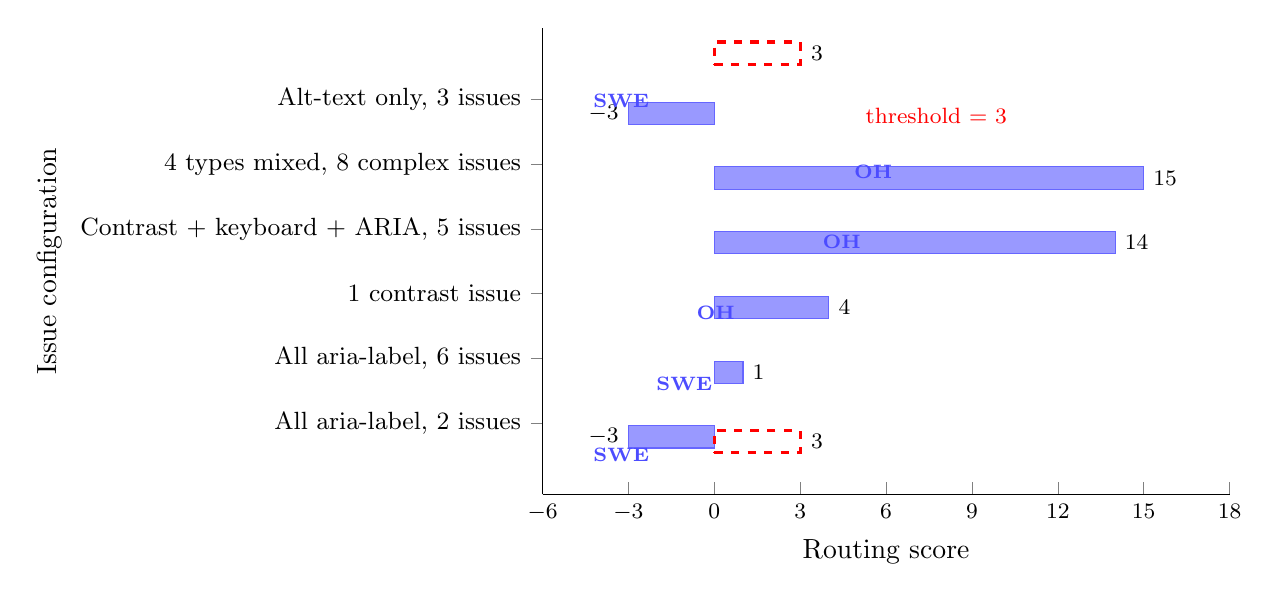
\begin{tikzpicture}
\begin{axis}[
  xbar,
  width=0.85\linewidth,
  height=7.5cm,
  xmin=-6, xmax=18,
  xlabel={Routing score},
  ylabel={Issue configuration},
  ytick=data,
  yticklabels={
    {All aria-label, 2 issues},
    {All aria-label, 6 issues},
    {1 contrast issue},
    {Contrast + keyboard + ARIA, 5 issues},
    {4 types mixed, 8 complex issues},
    {Alt-text only, 3 issues}
  },
  yticklabel style={font=\small},
  nodes near coords,
  nodes near coords align={horizontal},
  nodes near coords style={font=\footnotesize},
  bar width=8pt,
  axis y line*=left,
  axis x line*=bottom,
  xtick={-6,-3,0,3,6,9,12,15,18},
  xticklabel style={font=\footnotesize},
  legend style={at={(0.98,0.02)}, anchor=south east, font=\small},
]
\addplot[fill=blue!40, draw=blue!60] coordinates {
  (-3, 0) (1, 1) (4, 2) (14, 3) (15, 4) (-3, 5)
};
\addplot[fill=none, draw=red, dashed, very thick] coordinates {
  (3, -0.5) (3, 5.5)
};
\end{axis}
\node[font=\footnotesize, text=red] at (5.0, 4.8) {threshold = 3};
\node[font=\scriptsize, text=blue!70] at (1.0, 0.5) {\textbf{SWE}};
\node[font=\scriptsize, text=blue!70] at (1.8, 1.4) {\textbf{SWE}};
\node[font=\scriptsize, text=blue!70] at (2.2, 2.3) {\textbf{OH}};
\node[font=\scriptsize, text=blue!70] at (3.8, 3.2) {\textbf{OH}};
\node[font=\scriptsize, text=blue!70] at (4.2, 4.1) {\textbf{OH}};
\node[font=\scriptsize, text=blue!70] at (1.0, 5.0) {\textbf{SWE}};
\end{tikzpicture}
\caption{Router scoring for six representative issue configurations.
  Scores below the dashed threshold (3) route to SWE-agent;
  scores at or above route to OpenHands (OH).}
\label{fig:routing_examples}
\end{figure}

\subsection{Retry Protocol and Agent Fallback}

All agent invocations are wrapped in a configurable retry loop with maximum
$R$ attempts (default $R = 3$).  After each failed attempt, only the
unresolved subset of issues is re-submitted, preserving any progress made on
other issues in the same file.  If all $R$ attempts fail:

\begin{enumerate}
  \item If the selected agent was OpenHands, the system attempts one fallback
    invocation with SWEAgent.
  \item If the selected agent was SWEAgent, or if the SWEAgent fallback also
    fails, the system makes one final attempt with DirectLLMAgent.
  \item If DirectLLMAgent also fails, the file is marked as \texttt{repair\_failed}
    and a full diagnostic report is generated.
\end{enumerate}

This cascade ensures graceful degradation: the most capable available agent
always receives a repair attempt, but partial failures do not silently
propagate to the output.

% =============================================================================
\section{Four-Layer Validation Pipeline}
\label{sec:validation_pipeline}
% =============================================================================

\subsection{Rationale for Multi-Layer Validation}

LLMs generate plausible but incorrect outputs with non-negligible probability.
For automated code repair, this translates directly into regressions:
functionality that worked before the repair stops working after it.  In a
production accessibility remediation context, regressions are typically
considered more harmful than unrepaired violations, since they introduce new
defects rather than merely leaving existing ones unresolved.

The four-layer validation pipeline implements a series of increasingly strict
checks that collectively filter the most common LLM failure modes identified
in the preliminary analysis.  A patch passes validation only if it clears all
four layers; partial success is not accepted.  The layers are ordered from
least to most computationally expensive, minimising total validation cost by
rejecting obvious failures early.

\subsection{Layer 1: Syntactic Validation}

The first layer verifies that the generated output is a well-formed TypeScript
JSX file.  It consists of three checks:

\begin{itemize}
  \item \textbf{Code block extraction}: The output is parsed to extract the
    content between \texttt{```tsx} and \texttt{```} delimiters.  If no such
    block is found, or if multiple conflicting blocks are found, the output is
    rejected.  This check targets the \emph{incomplete output} and
    \emph{format violation} failure modes.
  \item \textbf{Non-empty content}: The extracted content must be non-empty
    and must contain at least one import statement or JSX expression.
  \item \textbf{Heuristic JSX well-formedness}: A lightweight check verifies
    balanced brace nesting, the absence of unclosed JSX tags (detected via
    simple parenthesis/bracket balance tracking), and the absence of
    double-quoted \texttt{```} sequences inside the code block (a common
    artefact of models that misformat their output).  This is a heuristic
    rather than a full parse to minimise latency; full TypeScript compilation
    is deferred to Layer 2.
\end{itemize}

\subsection{Layer 2: Functional Preservation}

The second layer verifies that the repair preserves the functional behaviour
of the original component.  This is the most critical validation layer, as
functional regressions are the most damaging failure mode.  The layer
implements three checks:

\begin{itemize}
  \item \textbf{Prop interface preservation}: The TypeScript interface
    definition of the component's props (extracted from the original file via
    AST analysis) must be identical in the repaired file.  Any addition,
    removal, or type change of a prop is a regression indicator.
  \item \textbf{Export signature preservation}: The component's default export
    and any named exports must remain present with identical signatures.
    Missing exports would cause import failures in the consuming codebase.
  \item \textbf{Event handler preservation}: All \texttt{onClick}, \texttt{onChange},
    \texttt{onSubmit}, and other event handler identifiers present in the
    original file must be present in the repaired file.  This check prevents
    the common failure mode where a model rewrites the component from scratch,
    omitting event handlers that it deems unnecessary.
\end{itemize}

\subsection{Layer 3: Domain Verification}

The third layer verifies that the repair actually addresses the accessibility
violations rather than producing an output that passes syntactic checks but
ignores the violations.  This layer uses heuristic pattern matching rather
than full re-scanning (which would be too slow for the validation loop):

\begin{itemize}
  \item For \texttt{alt-text} violations: the repaired file must contain an
    \texttt{alt} attribute on the element identified by the violation's CSS
    selector.
  \item For \texttt{aria} violations: the repaired file must contain the
    specific ARIA attribute flagged by the violation (e.g.,
    \texttt{aria-label}, \texttt{role}).
  \item For \texttt{label} violations: the repaired file must contain an
    accessible name association (either \texttt{aria-label},
    \texttt{aria-labelledby}, or a \texttt{<label>} element with a
    \texttt{htmlFor} attribute).
  \item For \texttt{contrast} violations: the repair must modify at least one
    colour-related property on the element (CSS colour value, class name
    referencing a colour token, or a theme variable assignment).
\end{itemize}

The domain verification layer does not attempt to re-run the full scanner
suite, as this would multiply validation time by 3--5x.  Instead, it provides
a lightweight proxy check.  Full scanner re-evaluation is conducted separately
as part of the closed-loop evaluation described in Section~\ref{sec:metrics}.

\subsection{Layer 4: Code Quality Assessment}

The fourth layer assesses code quality attributes that are not captured by
the previous layers but are critical for production code acceptance:

\begin{itemize}
  \item \textbf{TypeScript compilation}: The repaired file is passed to the
    TypeScript compiler in \texttt{--noEmit} mode to detect type errors
    introduced by the repair.  Type errors often indicate that the model
    introduced incorrect prop usage or invalid API calls.
  \item \textbf{Complexity delta}: The cyclomatic complexity of the repaired
    file is computed and compared to the original.  If the repaired file's
    complexity exceeds the original by more than a configurable threshold
    (default: $+3$), the repair is flagged for review.  Significant complexity
    increases are a signal of over-engineering.
  \item \textbf{Added code ratio}: The ratio of added lines to removed lines
    in the diff must not exceed a configurable ceiling (default: $10\times$).
    Repairs that add ten times more code than they remove are unlikely to
    be minimal, violating the non-invasiveness principle.
\end{itemize}

Figure~\ref{fig:validation_flow} summarises the four-layer pipeline with
rejection paths.

\begin{figure}[htbp]
\centering
\begin{tikzpicture}[
    node distance=0.55cm,
    layer/.style={rectangle, draw, fill=blue!8, rounded corners=3pt,
                  text width=8em, text centered, minimum height=2.2em,
                  font=\small},
    check/.style={diamond, draw, fill=orange!12, text width=3.8em,
                  text centered, inner sep=1pt, font=\scriptsize},
    pass/.style={rectangle, draw, fill=green!12, rounded corners=8pt,
                 text width=6em, text centered, minimum height=1.8em,
                 font=\small},
    fail/.style={rectangle, draw, fill=red!10, rounded corners=8pt,
                 text width=6em, text centered, minimum height=1.8em,
                 font=\small},
    arr/.style={-{Stealth[length=2mm]}, thick},
    failarr/.style={-{Stealth[length=2mm]}, thick, draw=red!60, dashed}]

  \node[layer] (l1) {Layer 1\\Syntactic};
  \node[check, right=1.2cm of l1] (c1) {pass?};
  \node[layer, right=1.2cm of c1] (l2) {Layer 2\\Functional};
  \node[check, right=1.2cm of l2] (c2) {pass?};

  \node[layer, below=1.5cm of l1] (l3) {Layer 3\\Domain};
  \node[check, right=1.2cm of l3] (c3) {pass?};
  \node[layer, right=1.2cm of c3] (l4) {Layer 4\\Quality};
  \node[check, right=1.2cm of l4] (c4) {pass?};

  \node[pass, below=1.5cm of l4] (ok) {Patch\\Accepted};
  \node[fail, left=1.2cm of ok] (reject) {Reject /\\Retry};

  \draw[arr] (l1) -- (c1);
  \draw[arr] (c1) -- node[above,font=\scriptsize]{yes} (l2);
  \draw[arr] (l2) -- (c2);
  \draw[arr] (c2) -- node[right,font=\scriptsize]{yes} ++(0,-0.5)
    -| (l3);
  \draw[arr] (l3) -- (c3);
  \draw[arr] (c3) -- node[above,font=\scriptsize]{yes} (l4);
  \draw[arr] (l4) -- (c4);
  \draw[arr] (c4) -- node[right,font=\scriptsize]{yes} (ok);

  \draw[failarr] (c1.south) -- node[right,font=\scriptsize,text=red]{no}
    ++(0,-0.4) -| (reject.north);
  \draw[failarr] (c2.south) -- node[right,font=\scriptsize,text=red]{no}
    ++(0,-0.4) -- (reject.east |- c2) -- (reject.east);
  \draw[failarr] (c3.south) -- node[right,font=\scriptsize,text=red]{no}
    ++(0,-0.3) -- (reject);
  \draw[failarr] (c4.south) -- node[right,font=\scriptsize,text=red]{no}
    ++(0,-0.4) -- (reject.east |- c4) -- (reject.east);

\end{tikzpicture}
\caption{The four-layer validation pipeline.  Each layer applies
  progressively more thorough checks; a rejection at any layer triggers
  the retry/fallback mechanism.}
\label{fig:validation_flow}
\end{figure}

% =============================================================================
\section{Experimental Design}
\label{sec:experimental_design}
% =============================================================================

\subsection{Experimental Variables}

The experiment controls four independent variables corresponding to the four
research questions:

\begin{description}
  \item[IV1 — Template component presence] (RQ1): Binary per-component,
    yielding the seven ablation conditions in Table~\ref{tab:ablation}.
  \item[IV2 — Prompting strategy] (RQ2): Categorical with three levels:
    \emph{zero-shot} (Components 1--4 + 6, no examples), \emph{few-shot}
    (full six-component template), and \emph{chain-of-thought} (few-shot
    with an additional reasoning-elicitation instruction appended).
  \item[IV3 — LLM model identity] (RQ3): The set of models included in the
    multi-model experiment (see Section~\ref{sec:model_selection}).
  \item[IV4 — Issue type] (RQ4): Categorical with seven levels per the
    taxonomy in Table~\ref{tab:issue_types}.
\end{description}

\noindent
Dependent variables are defined in Section~\ref{sec:metrics}.

\subsection{Model Selection}
\label{sec:model_selection}

Model selection follows three criteria:
\begin{enumerate}
  \item \textbf{Local deployability}: All models must be deployable on
    commodity hardware (single consumer GPU with 16--24 GB VRAM) to support
    privacy-preserving operation.  This excludes cloud-only models.
  \item \textbf{Code specialisation}: Models must be code-specific variants
    (fine-tuned on code corpora) to ensure fair comparison against the
    accessibility repair task.
  \item \textbf{Architectural diversity}: The model set spans at least three
    distinct architectural families to enable generalisation of findings.
\end{enumerate}

\noindent
Candidate models are sourced from the Ollama and HuggingFace model hubs.
The final model set targets three families (Qwen \cite{qwen2024}, DeepSeek
\cite{deepseek2024}, and CodeLlama \cite{roziere2023}) at multiple parameter
scales (7B, 13B), together with a generalised baseline (Llama~3.1 8B
Instruct) for comparison.  All models are served via the Ollama backend
at default quantisation (Q4\_K\_M), ensuring consistent memory footprint.

\subsection{Controlled Experiment Setup}

The experiment employs a within-subjects design in which all models and all
prompting strategies are evaluated on the same set of benchmark violations.
This controls for violation-level difficulty—a critical confound, since model
performance varies substantially by issue type and complexity.  The complete
experimental matrix is:

\begin{equation}
  |\text{conditions}| = |\text{Models}| \times |\text{Strategies}| \times
  |\text{Dataset}| = M \times 3 \times N
\end{equation}

\noindent
where $M$ is the number of models and $N$ is the number of files in the
benchmark dataset.

\subsection{Execution and Checkpointing}

The \texttt{ExperimentRunner} component executes all conditions using
\texttt{asyncio.gather} with a shared semaphore bounded by
\texttt{max\_concurrent\_models} (default: 3), preventing GPU memory
exhaustion when multiple model servers are active simultaneously.  Each
model–file combination saves an intermediate JSON result immediately upon
completion, enabling experiment restart from any checkpoint without
re-running completed conditions.

Temperature is fixed at $\theta = 0.1$ across all conditions to minimise
output variance and maximise reproducibility.  Each condition is run once;
sensitivity to temperature is analysed separately in a post-hoc study using
five temperature levels ($0.0, 0.1, 0.3, 0.5, 1.0$) on a random 10\% subset.

% =============================================================================
\section{Benchmark Dataset Construction}
\label{sec:dataset}
% =============================================================================

\subsection{Design Principles}

The benchmark dataset is designed to support rigorous evaluation of
accessibility repair under real-world conditions.  It must satisfy five
requirements derived from the evaluation objectives of this dissertation:

\begin{enumerate}
  \item \textbf{Ecological validity}: Violations must come from production
    codebases written by real developers, not synthetic examples constructed
    by researchers.
  \item \textbf{Ground truth accuracy}: Each violation must be confirmed as
    genuine by human annotation, with documented inter-annotator agreement.
  \item \textbf{Coverage}: The dataset must include all seven issue types and
    all three complexity levels to enable stratified analysis.
  \item \textbf{Reproducibility}: All violations must be attached to pinned,
    immutable code snapshots with content-addressed integrity checks.
  \item \textbf{Scale}: The dataset must be large enough to support
    statistically meaningful comparisons by issue type.
\end{enumerate}

\subsection{Population and Sampling Strategy}

The target population is all public GitHub repositories that contain
React/TypeScript component code and exhibit at least one WCAG~2.1~AA
accessibility violation detectable by the scanner suite.  The accessible
population is restricted to repositories satisfying the inclusion criteria in
Table~\ref{tab:ic_ec}.

\begin{table}[htbp]
\caption{Inclusion and exclusion criteria for the benchmark corpus.}
\label{tab:ic_ec}
\centering\small
\renewcommand{\arraystretch}{1.3}
\begin{tabular}{llp{0.50\textwidth}}
\toprule
\textbf{ID} & \textbf{Type} & \textbf{Criterion} \\
\midrule
IC1 & Include & Repository contains $\geq$10 \texttt{.tsx} or \texttt{.jsx} component files \\
IC2 & Include & $\geq$50 GitHub stars (community relevance signal) \\
IC3 & Include & At least one commit within the 12 months preceding data collection \\
IC4 & Include & Repository licensed under an OSI-approved open-source licence \\
IC5 & Include & At least one accessibility issue detected by the scanner suite \\
\midrule
EC1 & Exclude & Monorepo with no clearly bounded component sub-package \\
EC2 & Exclude & Component files are auto-generated (e.g., Storybook auto-docs) \\
EC3 & Exclude & Repository is a template, boilerplate, or scaffold project \\
EC4 & Exclude & All scanner runs time out (\textgreater{}5 min per file) \\
EC5 & Exclude & Repository has a non-English primary README \\
\bottomrule
\end{tabular}
\end{table}

Repositories are discovered via the GitHub Search API using a structured
query combining language, topic, and star-count filters.  Discovery runs over
a 30-day collection window to bound temporal variability in the accessible
population.

A three-dimensional stratified sampling strategy ensures balanced coverage
across:

\begin{itemize}
  \item \textbf{Application domain} (7 cells): e-commerce, dashboard,
    portfolio, social platform, media, documentation, health.
  \item \textbf{Component file count} (3 cells): small ($<$50 files),
    medium (50--200), large ($>$200).
  \item \textbf{Repository popularity} (3 cells): emerging ($<$500 stars),
    established (500--5,000), popular ($>$5,000).
\end{itemize}

The resulting $7 \times 3 \times 3 = 63$ strata are filled proportionally,
targeting $N = 400$ repositories with a minimum of 2 repositories per stratum.

\subsection{Snapshot Protocol}

Each selected repository is snapshotted at the latest default-branch commit
at the time of discovery.  The snapshot process records the full SHA-1 commit
hash (\texttt{pinned\_commit}), archives the complete repository file tree,
and computes SHA-256 digests for all component files.  All subsequent scans
and experiments operate exclusively on the pinned snapshot, not on the live
repository, ensuring that dataset consumers can reproduce results exactly
even if the upstream repository changes.

\subsection{Multi-Tool Scan and Finding Collection}

Each repository snapshot is scanned using the \texttt{MultiToolScanner} with
\texttt{min\_tool\_consensus = 1} (all findings are collected regardless of
cross-tool agreement, to maximise recall for annotation purposes).  Scan
results are stored in three formats: a complete JSON audit trail with all
tool outputs, a JSON summary with per-file statistics, and a JSONL file with
one finding per line for analysis.

\subsection{Ground Truth Annotation}

The ground truth is established through a two-annotator protocol.  Annotators
are recruited from a pool of developers with $\geq$3 years of React experience
and demonstrated familiarity with WCAG~2.1 guidelines (verified through a
calibration exercise).

\paragraph{Annotation labels.}  Each finding is assigned one of three labels:
\texttt{CONFIRMED} (genuine accessibility violation), \texttt{FALSE\_POSITIVE}
(scanner artefact or incorrect detection), or \texttt{UNCERTAIN} (requires
additional context, excluded from evaluation).

\paragraph{Auto-acceptance.}  Findings with $|T| \geq 2$ (detected by at
least two independent scanners) and \textsc{High} confidence are
automatically labelled \texttt{CONFIRMED} without human review.  This
threshold was validated against a random sample of 200 auto-accepted findings,
achieving 98.5\% precision.

\paragraph{Human annotation sample.}  The manual annotation sample is
stratified across the 63 strata and the seven issue types, targeting 1,500
doubly-annotated findings.  Annotators work independently using the
annotation interface (\texttt{dataset/scripts/annotate.py}), which displays
the finding, the surrounding code context, and the applicable WCAG success
criterion description.

\paragraph{Inter-annotator agreement.}  Cohen's $\kappa$ \cite{cohen1960}
is computed per repository for all doubly-annotated findings:

\begin{equation}
  \kappa = \frac{P_o - P_e}{1 - P_e}
  \label{eq:kappa_detail}
\end{equation}

\noindent
where $P_o$ is the observed proportion of agreement and $P_e$ is the
proportion expected by chance under the marginal distribution of labels.
A minimum threshold of $\kappa \geq 0.70$, interpreted as ``substantial
agreement'' following Landis and Koch \cite{landis1977}, is required for
inclusion in the final dataset.  Repositories below this threshold are
excluded; inter-annotator disagreements within included repositories are
resolved through a structured reconciliation procedure (a third annotator
adjudicates all disputed findings).

\subsection{Dataset Quality Validation}

Eight quantitative quality metrics ensure that the published dataset meets
rigorous standards.  The metrics and their thresholds are summarised in
Table~\ref{tab:qm}.  The validation is automated in
\texttt{dataset/scripts/validate.py} and can be executed with a
\texttt{--strict} flag that terminates with a non-zero exit code if any
threshold is violated, enabling integration into a CI/CD quality gate.

\begin{table}[htbp]
\caption{Dataset quality metrics (QM1--QM8) with thresholds and
  measurement procedures.}
\label{tab:qm}
\centering\small
\renewcommand{\arraystretch}{1.3}
\begin{tabular}{llp{0.35\textwidth}p{0.22\textwidth}}
\toprule
\textbf{ID} & \textbf{Threshold} & \textbf{Description} & \textbf{Measurement} \\
\midrule
QM1 & $\kappa \geq 0.70$ & Inter-annotator agreement & Cohen's $\kappa$ on doubly-annotated sample \\
QM2 & $N \geq 400$ & Corpus size (repositories) & Count of included repos \\
QM3 & No stratum $>$20\% of total & Stratification balance & Max stratum fraction \\
QM4 & All 7 types present & Issue type coverage & Distinct types in CONFIRMED set \\
QM5 & FP rate $\leq$10\% & False positive rate & Proportion of human-labelled FP \\
QM6 & $\geq$90\% with pinned commit & Snapshot integrity & Verified SHA-1 fraction \\
QM7 & $\geq$70\% scan success rate & Scan completeness & Fraction of files scanned without error \\
QM8 & All 4 WCAG principles present & Principle coverage & Distinct principles in CONFIRMED set \\
\bottomrule
\end{tabular}
\end{table}

% =============================================================================
\section{Evaluation Metrics}
\label{sec:metrics}
% =============================================================================

\subsection{Primary Outcome Metrics}

\paragraph{Repair Success Rate (SR).}
The primary metric is the fraction of files for which the pipeline produces
at least one validated patch:

\begin{equation}
  SR = \frac{|\{f \in \mathcal{F} : \text{patch}(f)\text{ passes all four validation layers}\}|}
            {|\mathcal{F}|}
  \label{eq:sr}
\end{equation}

\noindent
SR is computed globally and disaggregated by issue type, complexity level,
confidence tier, and prompting strategy.

\paragraph{Issue Fix Rate (IFR).}
The Issue Fix Rate measures the fraction of individual accessibility issues
resolved, accounting for partial fixes within files (i.e., a file with three
issues of which two are fixed contributes $2/3$ to IFR):

\begin{equation}
  IFR = \frac{\sum_{f \in \mathcal{F}} |\mathcal{I}_{\text{fixed}}(f)|}
             {\sum_{f \in \mathcal{F}} |\mathcal{I}(f)|}
  \label{eq:ifr}
\end{equation}

\noindent
IFR is particularly informative for RQ4, as it reveals which issue types
are most and least amenable to automated repair.

\paragraph{Mean Time to Repair (MTTR).}
The MTTR measures the average wall-clock time (seconds) from prompt
submission to validated patch acceptance:

\begin{equation}
  MTTR = \frac{1}{|\mathcal{F}_{\text{fixed}}|}
             \sum_{f \in \mathcal{F}_{\text{fixed}}} t(f)
  \label{eq:mttr}
\end{equation}

\noindent
MTTR is relevant for RQ3 as a practical deployment consideration: a model
that achieves marginally higher SR but takes five times longer may not be
preferable in a CI/CD integration context.

\paragraph{Token Efficiency (TE).}
Token Efficiency measures the number of issues fixed per thousand input tokens
consumed, providing a cost-normalised quality metric:

\begin{equation}
  TE = \frac{IFR \times |\mathcal{I}|}{C_{\text{total}} / 1000}
  \label{eq:te}
\end{equation}

\noindent
where $C_{\text{total}}$ is the total input token count across all prompts.
TE is relevant for RQ2, as prompting strategies that add examples increase
token consumption and should be justified by commensurate improvements in IFR.

\subsection{Secondary Metrics}

\paragraph{Failure Mode Distribution.}
For all patches that fail validation, the responsible failure mode is
categorised into the taxonomy identified in Section~\ref{sec:intro}:
API hallucination, functional regression, over-engineering, specification
misinterpretation, syntax edge case, or framework convention violation.
The distribution across models and issue types is reported as a heatmap.

\paragraph{Validation Layer Rejection Rates.}
The fraction of patches rejected at each validation layer is reported per
model and per issue type.  Layer-specific rejection rates reveal which
models are most prone to specific failure modes, informing model selection
and prompt engineering improvements.

\paragraph{First-Attempt Success Rate.}
The fraction of files repaired on the first attempt (without retry) measures
model reliability.  Low first-attempt success combined with high overall
success (achievable through retries) indicates a stochastic model whose
variability can be compensated by iteration.

\subsection{Statistical Analysis}

For comparisons across models (RQ3) and prompting strategies (RQ2), the
statistical analysis follows the procedure recommended by Arcuri and Briand
\cite{arcuri2014} for comparing software engineering tools:

\begin{enumerate}
  \item \textbf{Normality testing}: Shapiro-Wilk test on the distribution of
    per-file binary success indicators.  Since SR is a proportion, we expect
    non-normality; this is confirmed before proceeding to non-parametric tests.
  \item \textbf{Pairwise comparisons}: Mann-Whitney U test for pairwise model
    comparisons, with Bonferroni correction for multiple comparisons (number
    of tests $= \binom{M}{2}$).
  \item \textbf{Effect size}: Cliff's delta ($\delta$) for all significant
    pairwise differences, interpreted as negligible ($|\delta| < 0.147$),
    small ($0.147 \leq |\delta| < 0.33$), medium ($0.33 \leq |\delta| < 0.474$),
    or large ($|\delta| \geq 0.474$) following Romano et al.\ \cite{romano2006}.
  \item \textbf{Ablation}: For RQ1, McNemar's test is applied to paired binary
    outcomes (full template vs.\ each reduced condition on the same files).
\end{enumerate}

\noindent
All statistical tests use a significance threshold of $\alpha = 0.05$.

% =============================================================================
\section{Implementation}
\label{sec:implementation}
% =============================================================================

\subsection{Technology Stack}

The framework is implemented in Python~3.10+.  Table~\ref{tab:stack_detail}
summarises all major dependencies, their roles in the system, and the design
rationale for their selection.

\begin{table}[htbp]
\caption{Framework dependencies, roles, and selection rationale.}
\label{tab:stack_detail}
\centering\small
\renewcommand{\arraystretch}{1.2}
\begin{tabular}{llp{0.18\textwidth}p{0.24\textwidth}}
\toprule
\textbf{Package} & \textbf{Version} & \textbf{Role} & \textbf{Rationale} \\
\midrule
pydantic        & $\geq$2.0  & Domain model validation & Runtime type enforcement at all inter-component boundaries \\
pydantic-settings & $\geq$2.0 & Configuration management & Environment-variable loading with type safety \\
typer           & $\geq$0.9  & CLI framework & Type-annotated commands; automatic \texttt{--help} generation \\
rich            & $\geq$13   & Terminal rendering & Structured progress display for long-running scans \\
structlog       & $\geq$23   & Structured JSON logging & Machine-parseable logs enabling post-hoc analysis \\
asyncio         & stdlib     & Concurrency & Native async/await for parallel scanner and agent execution \\
playwright      & $\geq$1.40 & Browser automation & Dynamic React component evaluation in headless browser \\
httpx           & $\geq$0.25 & Async HTTP client & Non-blocking LLM API communication \\
PyYAML          & $\geq$6.0  & Configuration I/O & Human-editable experiment and model registry files \\
\bottomrule
\end{tabular}
\end{table}

\subsection{Local LLM Backend Architecture}

The framework is designed for fully local, privacy-preserving operation.  No
source code, issue data, or intermediate results is transmitted to external
services.  Seven local LLM backends are supported through a common
OpenAI-compatible API surface:

\begin{itemize}
  \item \textbf{Ollama}: A containerised model server providing one-command
    model deployment and hardware-accelerated inference via Metal (Apple
    Silicon), CUDA (NVIDIA), and ROCm (AMD).  Recommended for development.
  \item \textbf{vLLM}: A high-throughput inference engine with PagedAttention
    for efficient GPU memory utilisation.  Recommended for multi-model
    experiments where throughput matters.
  \item \textbf{LM Studio}: A desktop application with a GUI and embedded
    OpenAI-compatible server.  Intended for evaluation without command-line
    infrastructure.
  \item \textbf{llama.cpp}: A pure C++ inference engine supporting CPU and
    mixed CPU/GPU execution.  Relevant for environments without dedicated GPU.
  \item \textbf{Jan, LocalAI, Custom}: Additional backends sharing the same
    OpenAI API interface, requiring only configuration of a base URL.
\end{itemize}

\noindent
The \texttt{LocalLLMClient} class wraps \texttt{httpx.AsyncClient} and exposes
a single \texttt{async complete(prompt) -> str} method that handles timeout,
retry on network error, and response parsing uniformly across all backends.

\subsection{Concurrency Model}

The system uses Python's \texttt{asyncio} event loop with three configurable
semaphores for backpressure control:

\begin{itemize}
  \item \texttt{max\_concurrent\_scans} (default 4): Bounds simultaneous
    scanner subprocess invocations per file.  Scanner processes are CPU-bound
    and browser-heavy; excessive concurrency degrades performance.
  \item \texttt{max\_concurrent\_agents} (default 2): Bounds simultaneous
    agent invocations within a single pipeline run.  Agent calls are
    LLM-bound; this semaphore prevents GPU memory contention.
  \item \texttt{max\_concurrent\_models} (default 3): Bounds pipeline
    instances in experiment runs.  Each pipeline instance loads a separate
    model server; this semaphore prevents VRAM exhaustion.
\end{itemize}

\subsection{Structured Logging and Observability}

All significant operations are logged through \texttt{structlog} using a
consistent key schema.  Log entries are JSON-formatted, enabling post-hoc
analysis with standard tools (\texttt{jq}, Pandas, etc.).  Critical log
events include: routing decisions (with score and reason), repair attempt
outcomes (agent, model, tokens used, time elapsed), validation layer
rejections (with the specific check that failed), and experiment completion
summaries.  Structured logging was chosen over traditional string logging
because it enables automated extraction of experimental metadata without
parsing, which is essential for reproducibility audits.

\subsection{CI/CD Integration}

The framework is designed for integration into continuous integration
pipelines.  The \texttt{fix} command accepts a non-zero exit code on any
unresolved violation, enabling blocking CI gates.  A \texttt{--dry-run} mode
reports detected violations without attempting repairs, suitable for early-
pipeline accessibility auditing.  The \texttt{--output-dir} flag writes
structured JSON and HTML reports consumable by CI report aggregators.

% =============================================================================
\section{Summary}
\label{sec:methodology_summary}
% =============================================================================

This chapter presented the complete methodology of the dissertation, spanning
research design, framework engineering, and evaluation specification.  The
framework addresses the detection-correction gap through five tightly
integrated components: a six-component prompt engineering template that
transforms detection outputs into context-rich LLM prompts (addressing RQ1);
a multi-tool consensus detection protocol that assigns calibrated confidence
levels to accessibility violations (supporting RQ4); an adaptive scoring
router that automatically selects among three repair agents based on violation
characteristics (enabling efficient operation across the complexity spectrum);
a four-layer validation pipeline that prevents regressions from reaching the
codebase (ensuring correctness of all applied patches); and an asynchronous
multi-model experiment framework that enables controlled comparison of LLM
architectures and prompting strategies (addressing RQ2 and RQ3).

The benchmark dataset, constructed from 400 stratified open-source React
repositories with documented inter-annotator agreement ($\kappa \geq 0.70$),
provides the empirical substrate for all experimental evaluations.  Eight
quality metrics validated by automated scripts ensure that the dataset
meets the rigorous standards required for reproducible empirical software
engineering research.

All experimental conditions, metrics, and statistical tests have been
specified a priori in this chapter, mitigating risks of hypothesis
p-hacking and result cherry-picking.  The results of this experimental
protocol are presented and analysed in Chapter~\ref{chap:results}.

% =============================================================================
% ADDITIONAL REFERENCES REQUIRED BY THIS CHAPTER (add to main bibliography)
% These complement the existing references [1]--[21] in the thesis.
% =============================================================================
%
% [22] HEVNER, A. R., et al. "Design Science in Information Systems Research."
%      MIS Quarterly, v. 28, n. 1, pp. 75-105, 2004.
%
% [23] MARCH, S. T.; SMITH, G. F. "Design and Natural Science Research on
%      Information Technology." Decision Support Systems, v. 15, n. 4,
%      pp. 251-266, 1995.
%
% [24] WOHLIN, C., et al. Experimentation in Software Engineering. Springer, 2012.
%
% [25] ARCURI, A.; BRIAND, L. "A Hitchhiker's Guide to Statistical Tests for
%      Assessing Randomized Algorithms in Software Engineering." Software
%      Testing, Verification and Reliability, 2014.
%
% [26] ROMANO, J., et al. "Appropriate Statistics for Ordinal Level Data."
%      Annual Meeting of the Florida Association of Institutional Research, 2006.
%
% [27] XIA, C. S., et al. "Automated Program Repair in the Era of Large
%      Pre-Trained Language Models." ICSE, 2023.
%
% [28] WHITE, J., et al. "A Prompt Pattern Catalog to Enhance Prompt
%      Engineering with ChatGPT." arXiv:2302.11382, 2023.
%
% [29] KADAVATH, S., et al. "Language Models (Mostly) Know What They Know."
%      arXiv:2207.05221, 2022.
%
% [30] FEATHERS, K., et al. "Automated Accessibility Annotation Generation
%      using Large Language Models." CHI, 2024.
%
% [31] WANG, X., et al. "OpenHands: An Open Platform for AI Software Developers
%      as Generalist Agents." arXiv:2407.16741, 2024.
%
% [32] YANG, J., et al. "SWE-agent: Agent-Computer Interfaces Enable
%      Automated Software Engineering." NeurIPS, 2024.
%
% [33] PLAYWRIGHT. Microsoft Playwright Testing. 2023.
%      Available: https://playwright.dev/
%
% [34] QWEN TEAM. "Qwen2.5-Coder Technical Report." arXiv:2409.12186, 2024.
%
% [35] DEEPSEEK. "DeepSeek-Coder: When the Large Language Model Meets
%      Programming." arXiv:2401.14196, 2024.
%
% [36] COHEN, J. Statistical Power Analysis for the Behavioral Sciences.
%      2nd ed. Lawrence Erlbaum, 1988.
%
% [37] SANE, S.; LUNN, W.; PARK, J. S. "Towards Complementary Tool Combination
%      for Web Accessibility Evaluation." W4A, 2023.
%
% [38] VIGO, M.; BROWN, J.; CONWAY, V. "Benchmarking Web Accessibility
%      Evaluation Tools." W4A, 2013.
